\chapter{Beyond Leading Log with High Energy Jets}

Now that the driving principles behind HEJ have been explained, we move on to discuss recent improvements to the formalism. We begin by discussing how the form of our amplitudes allows us to also capture terms that are Next-to-Leading Logarithmic (NLL) in the perturbative series. We will go into the motivations for why we should do this before presenting a full description of how some of these terms are derived and incorporated. We then finalise the chapter by presenting new results clearly showing the beneficial effect of the addition of these contributions, both in terms of the HEJ program and in comparison to real LHC data. 

\section{Motivations for NLL}

There are a few reasons one might consider trying to go beyond LL with the formalism. Firstly, it has been proved that the Lipatov ansatz is valid at the NLL level \cite{Fadin2006} and so any sub-leading amplitude that still factors out into a product of $t$-channel poles can be resummed in the same way as before. The full form of the trajectory $\hat{\alpha}$, which we derived at the leading order in section 2.1.1, of course becomes more complicated \cite{Fadin2003}, but the important point is that the form of the Lipatov ansatz (equation \ref{eqn:lipansatz}) still holds. Secondly, by having access to these sub-leading terms we also expect to reduce the scale variation bands on our calculation, since these variations are directly related to how much control we have over higher order terms. In order to claim full NLL accuracy, we must have:

\begin{enumerate}
\item{Calculations of FKL amplitudes but with the rapidity ordering of one emitted gluon disturbed (one gluon is allowed to be emitted with a rapidity that is outside of an extremal parton). We call such contributions `unordered' processes.}
%\item{Implementation of the full form of the next-to-leading expression for $\hat{\alpha}$.}
\item{Corrections to the Lipatov vertex for the emission of gluons.}
\item{Calculations of inherently non-FKL amplitudes (those which cannot be drawn with only $t$-channel gluon exchanges) that contribute at the NLL level in the jet cross-section.}
\end{enumerate}

%\todo{talk more about uno here}
The mathematics of the first point had already been completed and the author's contribution to this project was to incorporate these routines in the HEJ program's pure jet production section. The second point has not yet been attempted but remains a long-term goal of the collaboration. This thesis will consider the first and final points, providing a brief overview of the former and a complete description and derivation of the author's individual work for the latter. Including such considerations will mark an important step towards full NLL HEJ and, in the case of the addition of the non-FKL subprocesses, it extends the applicability of HEJ since we will now have a LL description of these events; in conclusion, we will be able to resum more of the contribution to the cross-section. 

\section{Unordered Emissions in Pure Jets}
%\todo{Uno section! Or incorporated into last section?}
The derivation of the amplitude for an unordered (or simply `uno') contribution revolves around extending our current formalism to include the effect of a gluon being emitted outside the FKL strongly rapidity-ordered chain. We can express this by introducing a modified current object that depends on the rapidity of this unordered parton and the parton next to it in rapidity that does satisfy the ordering. For example, the amplitude for $qQ \to gqQ$ would behave as
\begin{equation}
M_{qQ \to gqQ}^{uno} \sim \frac{j^\mu_{uno}(p_a,p_1,p_{uno})j_\mu(p_b,p_2)}{\hat{t}_2},
\label{eqn:uno}
\end{equation}
\begin{figure}[t]
\centering
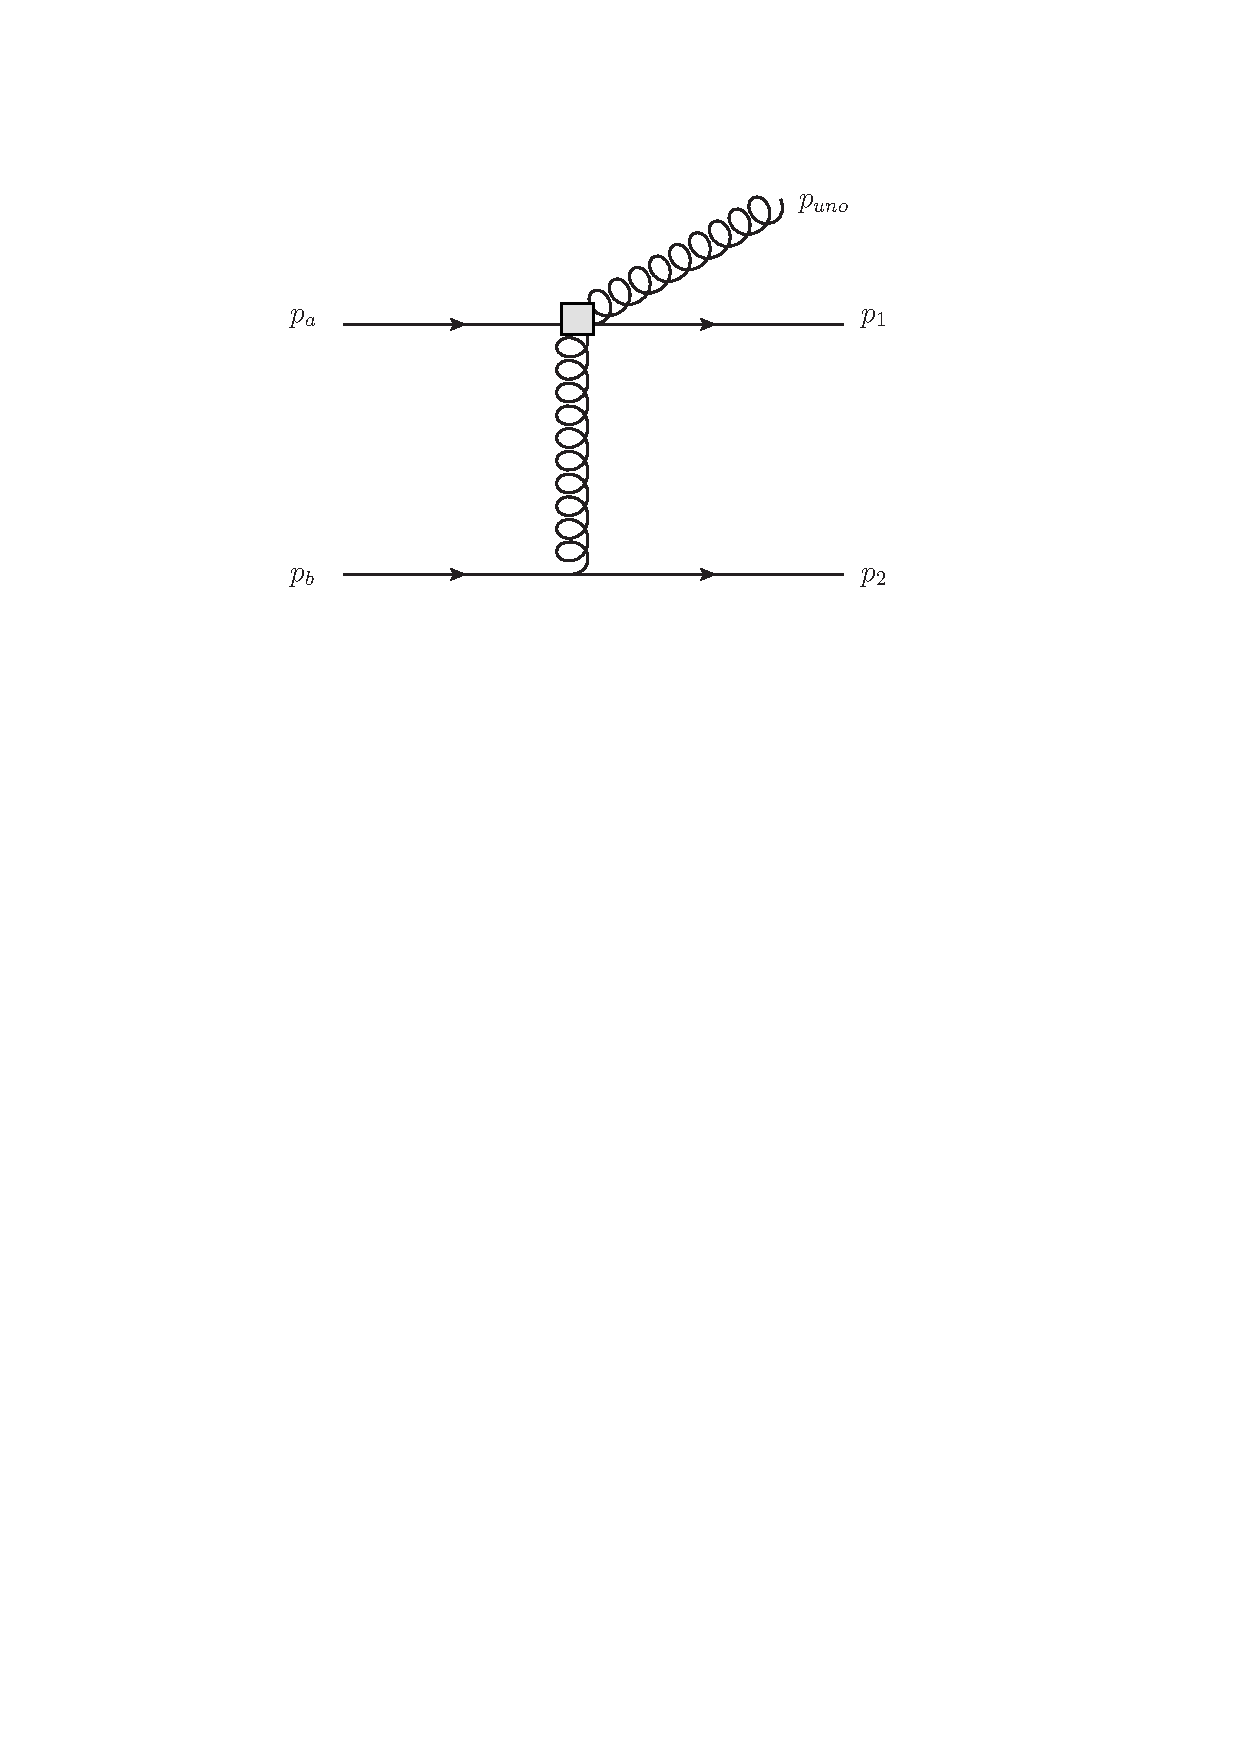
\includegraphics[scale=0.7]{Images/uno.pdf}
\caption{A schematic view of an unordered emission amplitude.}
\label{fig:uno}
\end{figure}

where $y_{uno} \sim y_1$ and $y_1 \gg y_2$. Throughout the following sections, we will make clear where $t$-channel poles appear by employing the notation $\hat{t}_i = p_a - \sum_{j=1}^{j=i} p_j$ and such invariants will \emph{always} be factored out of the final expression. For other instances where the use of a $t$-channel propagator still makes sense, we use the notation $t_{ij}$, which is to be interpreted as $(p_i-p_j)^2 = -s_{ij}$.  Returning to the unordered amplitude and in essence, we collapse the gluon emission to a point along the usual current such that there is only one suitable $t$-channel pole to be resummed, as opposed to the two we would get if the gluon were emitted in the FKL ordering -- it is thus clear to see why this is a sub-leading contribution. Diagrammatically, we can represent this as shown in figure \ref{fig:uno}. We should also keep in mind that discussing the colour properties of this amplitude will be more complicated than the FKL case and the result will have to be treated more carefully in this regard. To derive the form of the uno current, we will recalculate the $qQ \to gqQ$ amplitude but with the consideration that the rapidity of the gluon is no longer far away from the rapidity of the forward quark current. What this will essentially mean is that the kinematic arguments for dropping some terms, as was done in section 2.2.3, will no longer be valid. We will therefore start by writing the full LO result for this amplitude (where we will write $p_{uno} = p_g$ for brevity):
\begin{equation}
\begin{split}
M_{qQ \to gqQ}^{LO} =& (ig_s)^3 T^c_{1i}T_{ia}^d T^d_{2b} \varepsilon_{\nu}(p_g) \frac{\matel{1}{\nu}{g}\matel{g}{\mu}{a} + 2p_1^\nu \matel{1}{\mu}{a}}{s_{1g}\hat{t}_2}\matel{2}{\mu}{b} \\
 &- (ig_s)^3 T^d_{1i}T_{ia}^c T^d_{2b} \varepsilon_{\nu}(p_g) \frac{2p_a^\nu \matel{1}{\mu}{a} - \matel{1}{\mu}{g}\matel{g}{\nu}{a}}{s_{ag}\hat{t}_2}\matel{2}{\mu}{b} \\
 &+ (ig_s)^3 T^c_{2i}T_{ib}^d T^d_{1a} \varepsilon_{\nu}(p_g) \frac{\matel{2}{\nu}{g}\matel{g}{\mu}{b} + 2p_2^\nu \matel{2}{\mu}{b}}{s_{2g}t_{a1}}\matel{1}{\mu}{a} \\
  &- (ig_s)^3 T^d_{2i}T_{ib}^c T^d_{1a} \varepsilon_{\nu}(p_g) \frac{2p_b^\nu \matel{2}{\mu}{b} - \matel{2}{\mu}{g}\matel{g}{\nu}{b}}{s_{bg}t_{a1}}\matel{1}{\mu}{a} \\
  &-g_s^3 f^{dec}T^d_{1a}T^e_{2b} \varepsilon_\nu(p_g) \frac{\matel{1}{\rho}{a}\matel{2}{\mu}{b}}{t_{a1} \hat{t}_2}(2p_g^\mu \eta^{\nu \rho} - 2p_g^\rho \eta^{\mu \nu} - (q_1 + q_2)^\nu \eta^{\mu \rho}),
\end{split}
\end{equation}
where $q_1 = p_a - p_1 = p_2 - p_b + p_g$ and $q_2 = p_2 - p_b = p_a - p_1 - p_g$. With the full expression available, we can investigate which terms we can still drop in this new limit $y_g \sim y_1 \gg y_2$. We see that the first term in the third line and the second term in the fourth are the only ones we can drop because (depending on helicities) the $\mu$ contraction will give something that scales as $\sqrt{s_{ag}}$ or $\sqrt{s_{g1}}$, which are now small invariants in comparison to all other scales. By dropping these terms, all remaining terms are proportional to $\matel{2}{\mu}{b}$ and so by comparison to equation \ref{eqn:uno}, the sum of the terms multiplying this current will give us our unordered current. However, to be truly consistent with the factorised picture, we must factorise out the colour factor $T^d_{2b}$ from this amplitude as well. This is already the case for the first, second and last lines and now that we have dropped terms for the other two lines we can use the (still valid) limit $p_2 \sim p_b$ to yield
\begin{equation}
\begin{split}
& -ig_s^3 \matel{1}{\mu}a{} \matel{2}{\mu}{b} \varepsilon_\nu(p_g) \left(\frac{2p_2^\nu}{t_{a1} s_{2g}} - \frac{2p_b^\nu}{t_{a1} s_{bg}} \right) \\
& \approx -i g_s^3 \matel{1}{\mu}{a} \matel{2}{\mu}{b} \varepsilon_\nu(p_g) \frac{1}{t_{a1}}\frac{2p_b^\nu}{s_{bg}} T^d_{1a}\left(T^c_{2i}T^d_{ib} - T^d_{2i}T^c_{ib}\right)  \\
&= g_s^3 \matel{1}{\mu}{a} \matel{2}{\mu}{b} \varepsilon_\nu(p_g) \frac{1}{t_{a1}} \frac{2 p_b^\nu}{s_{bg}} f^{cde}T^d_{1a}T^e_{2b} \\
&= g_s^3 \matel{1}{\mu}{a} \matel{2}{\mu}{b} \varepsilon_\nu(p_g) f^{cde}T^d_{1a}T^e_{2b} \frac{1}{t_{a1}} \left(\frac{p_b^\nu}{s_{bg}}+\frac{p_2^\nu}{s_{2g}} \right),
\end{split}
\end{equation}
where in the last line we have restored the symmetry between $p_2$ and $p_b$. Our factorised amplitude is then
\begin{equation}
M_{qQ \to gqQ}^{uno, fact} = -g_s^3 \frac{\matel{2}{\mu}{b}}{\hat{t}_2}T_{2b}^d \left(iT^c_{1i}T^d_{ia}U_1^{\mu \nu} + iT^d_{1i}T^c_{ia}U_2^{\mu \nu} + f^{ecd}T^e_{1a}L^{\mu \nu} \right),
\end{equation}
where
\begin{equation}
\begin{split}
U_1^{\mu \nu} &= \frac{1}{s_{1g}}(j^\nu_{1g}j^\mu_{ga} + 2 p_1^\nu j^\mu_{1a}) \\
U_2^{\mu \nu} &= -\frac{1}{s_{ag}}(2j^\mu_{1a}p_a^\nu - j^\mu_{1g}j^\nu_{ga}) \\
L^{\mu \nu} &= \frac{1}{t_{a1}} \left(-2p^\mu_g j^\nu_{1a} + 2 p_g \cdot j_{1a}\eta^{\mu \nu} + (q_1 + q_2)^\nu j^{\mu}_{1a} + q_2^2 j^\mu_{1a} \left(\frac{p_2^\nu}{s_{2g}} + \frac{p_b^\nu}{s_{gb}} \right) \right).
\end{split}
\end{equation}
%The three colour factors are not independent here, so we can combine them and then we can extract the uno current by inspection; \todo{Skip this?}
%\begin{equation}
%j^\mu_{uno}(p_1, p_a, p_g) = i \varepsilon_\nu(p_g) \left(T^c_{1i}T^d_{ia}\left(U_1^{\mu \nu} - L^{\mu \nu}\right) + T^d_{1i}T^c_{1a}\left(U_2^{\mu \nu} + L^{\mu \nu}\right) \right).
%\end{equation}
Gauge invariance of this expression has been checked by replacing the polarisation vector with the gluon momentum and seeing that the expression gives zero, in accordance with the Ward Identity. This current can then be used as a basis for all unordered amplitudes, with further emissions included via the Lipatov vertex and other incoming states accounted for by multiplications of $C_F$ and $\tilde{C}_A$ as appropriate. One thing to note, however, is that the leg that the unordered current is dependent on cannot be a gluon, since a trivial rewriting of momenta in that case will lead back to the FKL ordering. 

\section{Calculations of NLL Partonic Subprocesses}

It was discussed in chapter 2 that the dominant amplitudes in the High Energy Limit are given by those that involve the maximal number of gluon exchanges in the $t$-channel by analysis of Regge Theory. To access the sub-leading partonic configurations, we simply replace one gluon propagator by one quark propagator in these FKL amplitudes (whilst keeping the strict rapidity ordering). There are two distinct possibilities we can imagine: we can either replace the first or last propagator in the chain, or one in the middle along the chain. We can assign the nomenclature `extremal' and `central' to the two cases respectively. The simplest case of an extremal process is $qg \to qQ\bar{Q}$ and for the central case it is $qq' \to qQ\bar{Q}q'$. From analysis of these amplitudes, we can derive the `building blocks' that will allow us to build up other, related amplitudes by multiplication of Lipatov vertices and colour factors. 

\subsection{Calculation of $qg \to qQ\bar{Q}$ in the High Energy Limit}

The ultimate aim of this calculation will be to factorise the $qg \to qQ\bar{Q}$ amplitude into an expression of the form
\begin{equation}
M_{qg \to qQ\bar{Q}} \sim \frac{\matel{1}{\mu}{a}Q^{\mu \nu}(p_2, p_3, p_b) \varepsilon_\nu(p_b)}{\hat{t}_1},
\label{eqn:NLLeqn}
\end{equation}
where $Q^{\mu \nu}$ is an effective vertex that encapsulates the effect of the emission of a quark/anti-quark pair at the end of the rapidity chain. We can express this equation in the form a diagram; see figure \ref{fig:qgimp}. Given the momentum dependence of the vertex and how it looks schematically, we can also interpret $Q^{\mu \nu}$ as a $g \to Q \bar{Q}$ \emph{impact factor}.

\begin{figure}[t]
\centering
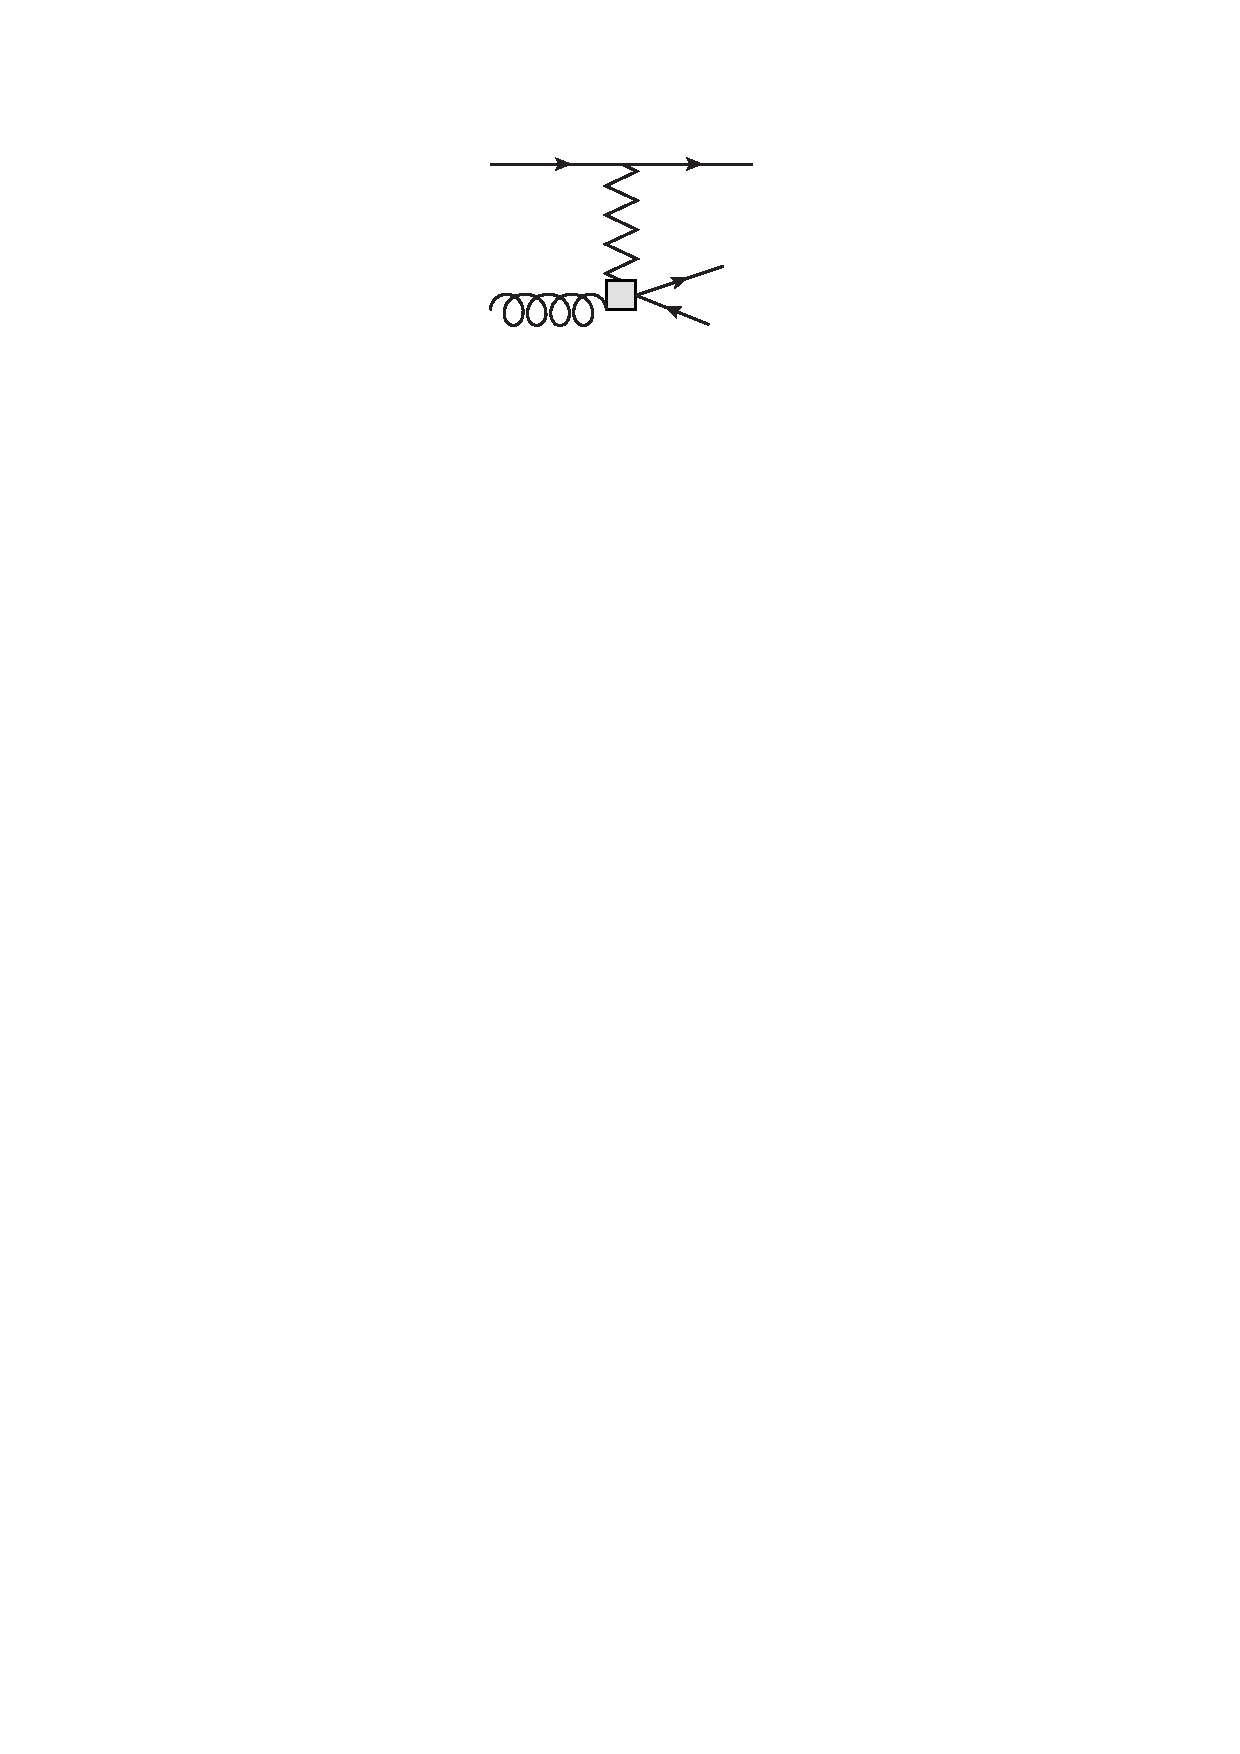
\includegraphics{Images/g_q_qbar_imp.pdf}
\caption{Schematic diagram involving $g \to q \bar{q}$ impact factor.}
\label{fig:qgimp}
\end{figure}

\begin{figure}[t] 
\centering
\subfloat{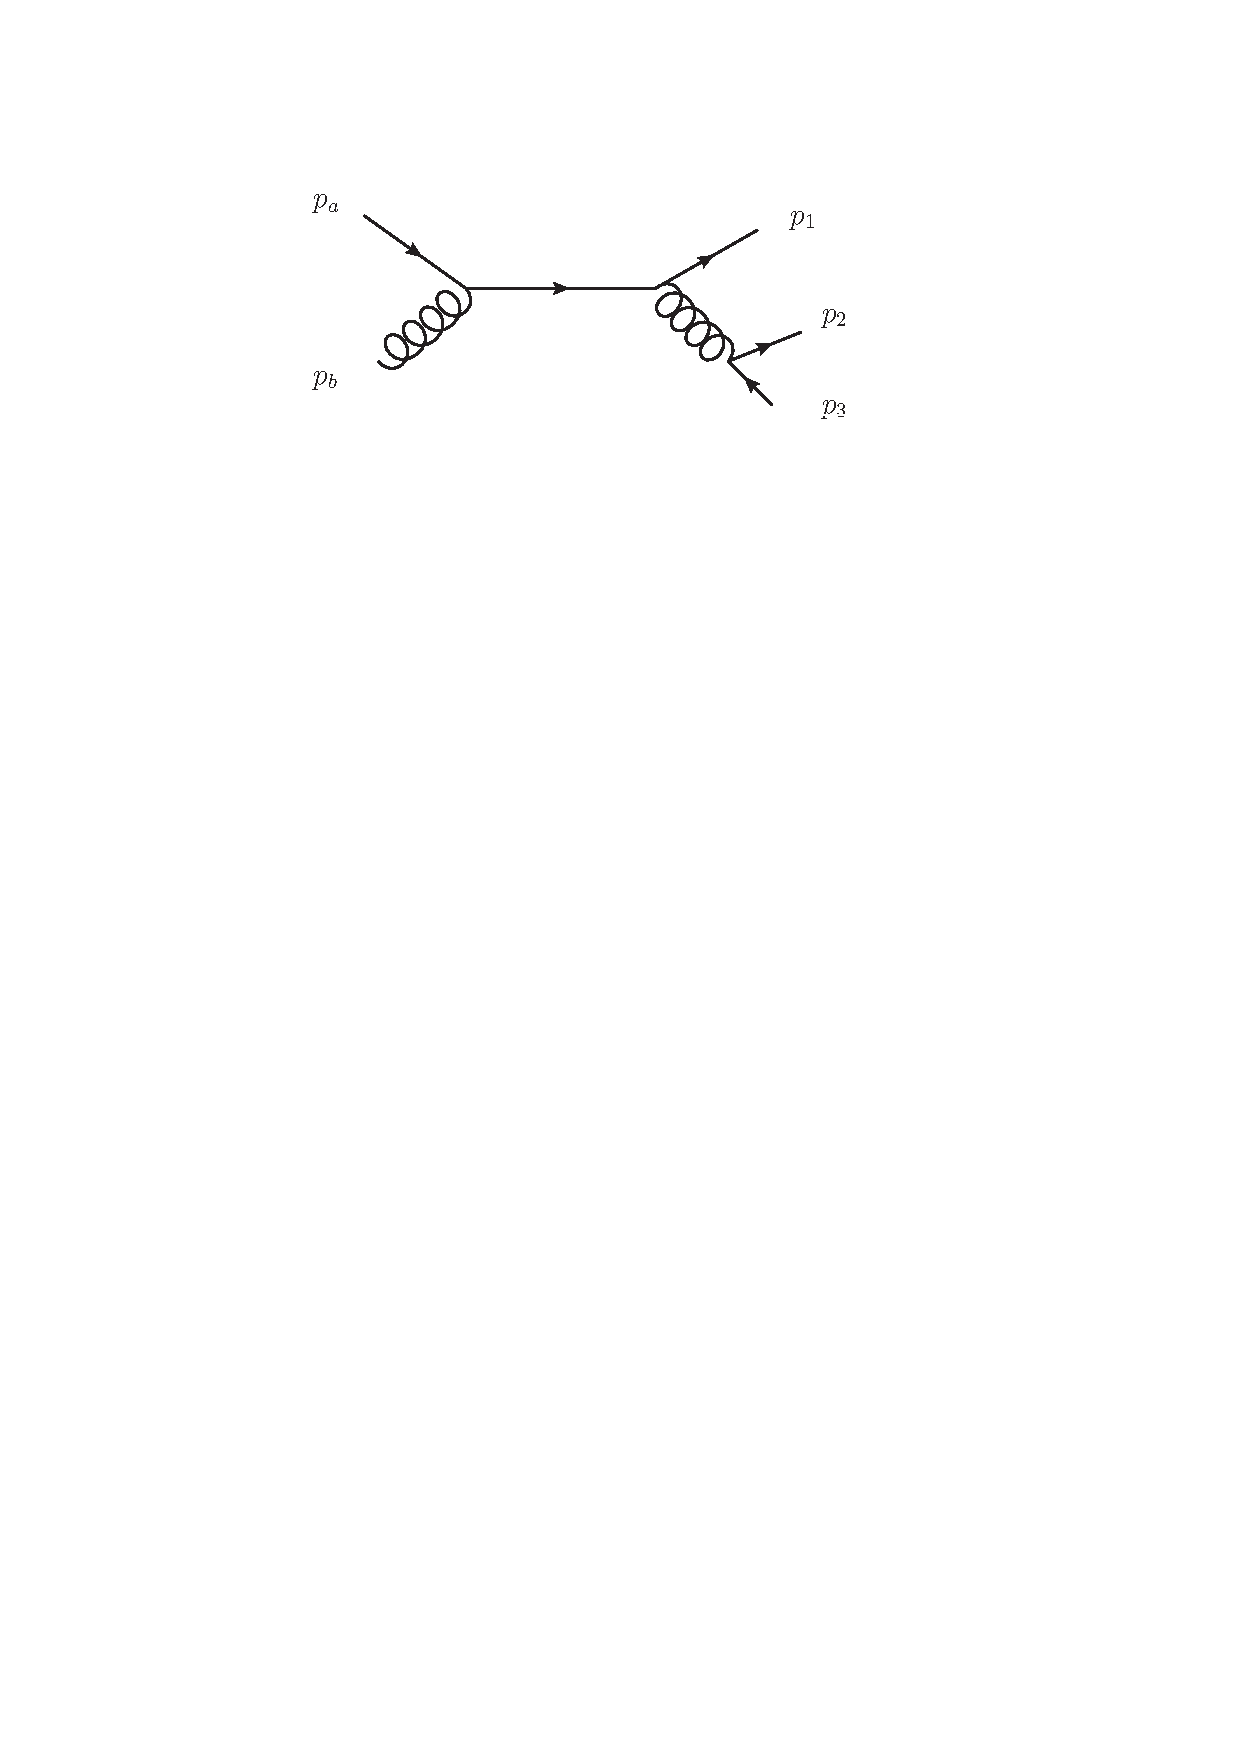
\includegraphics[scale=0.8]{Images/qg_qQQbar_s.pdf}} 
\subfloat{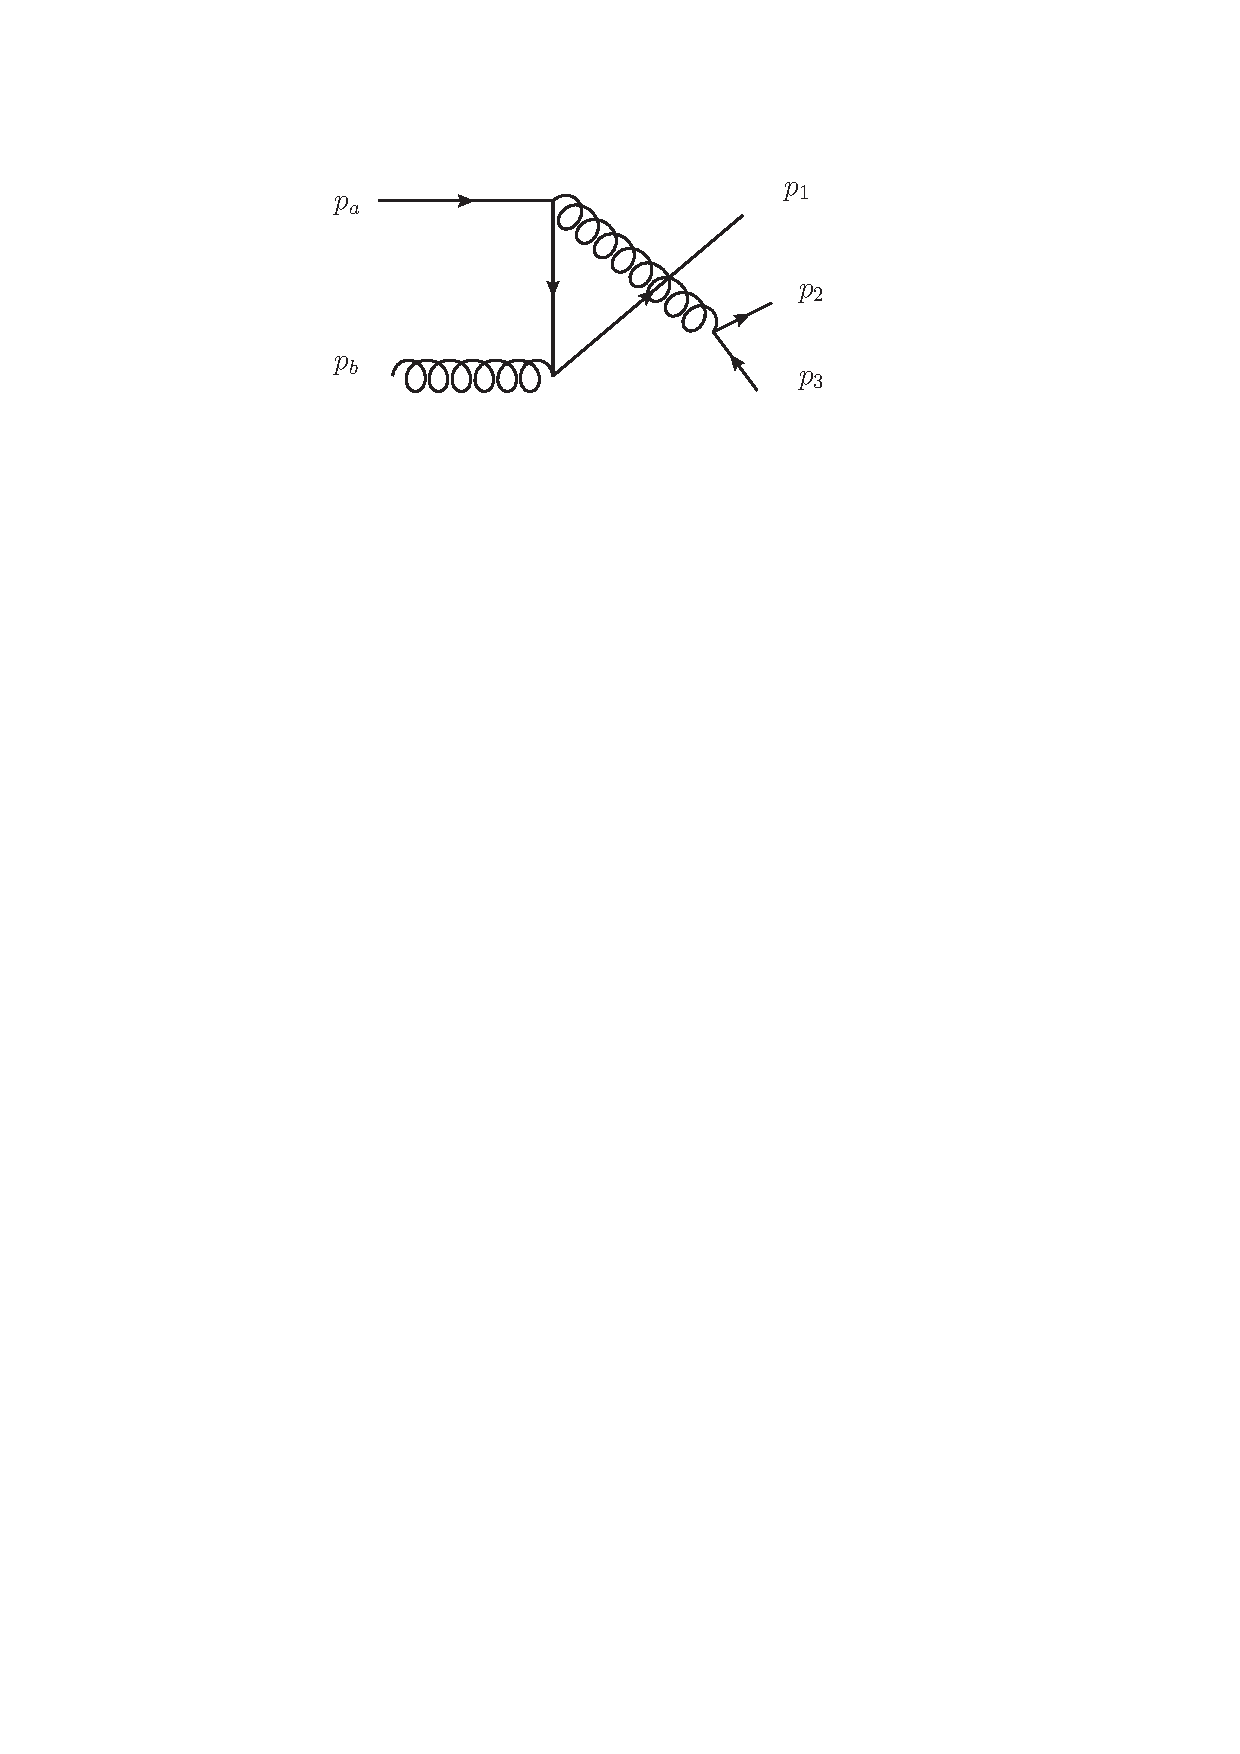
\includegraphics[scale=0.8]{Images/qg_qQQbar_u.pdf}} \\
\subfloat{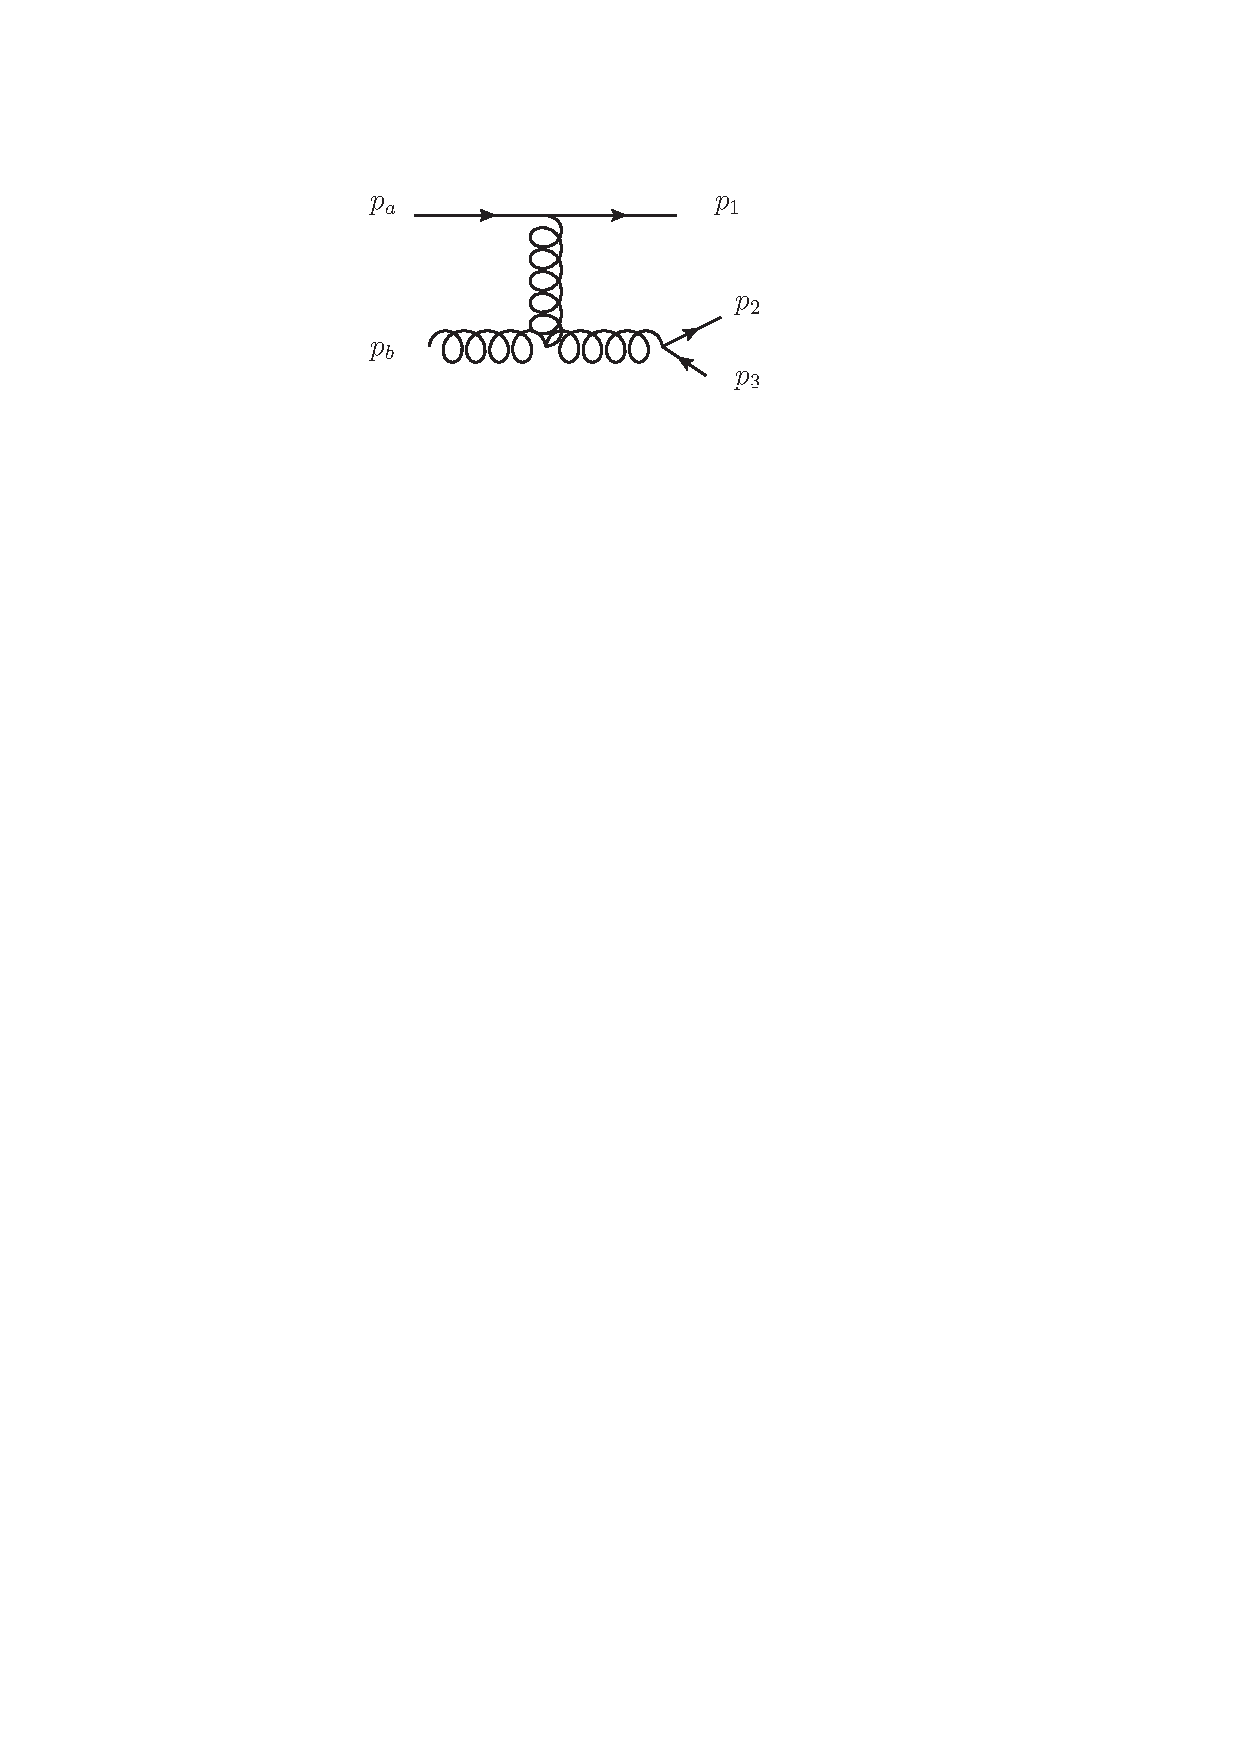
\includegraphics[scale=1]{Images/qg_qQQbar_t.pdf}} 
\subfloat{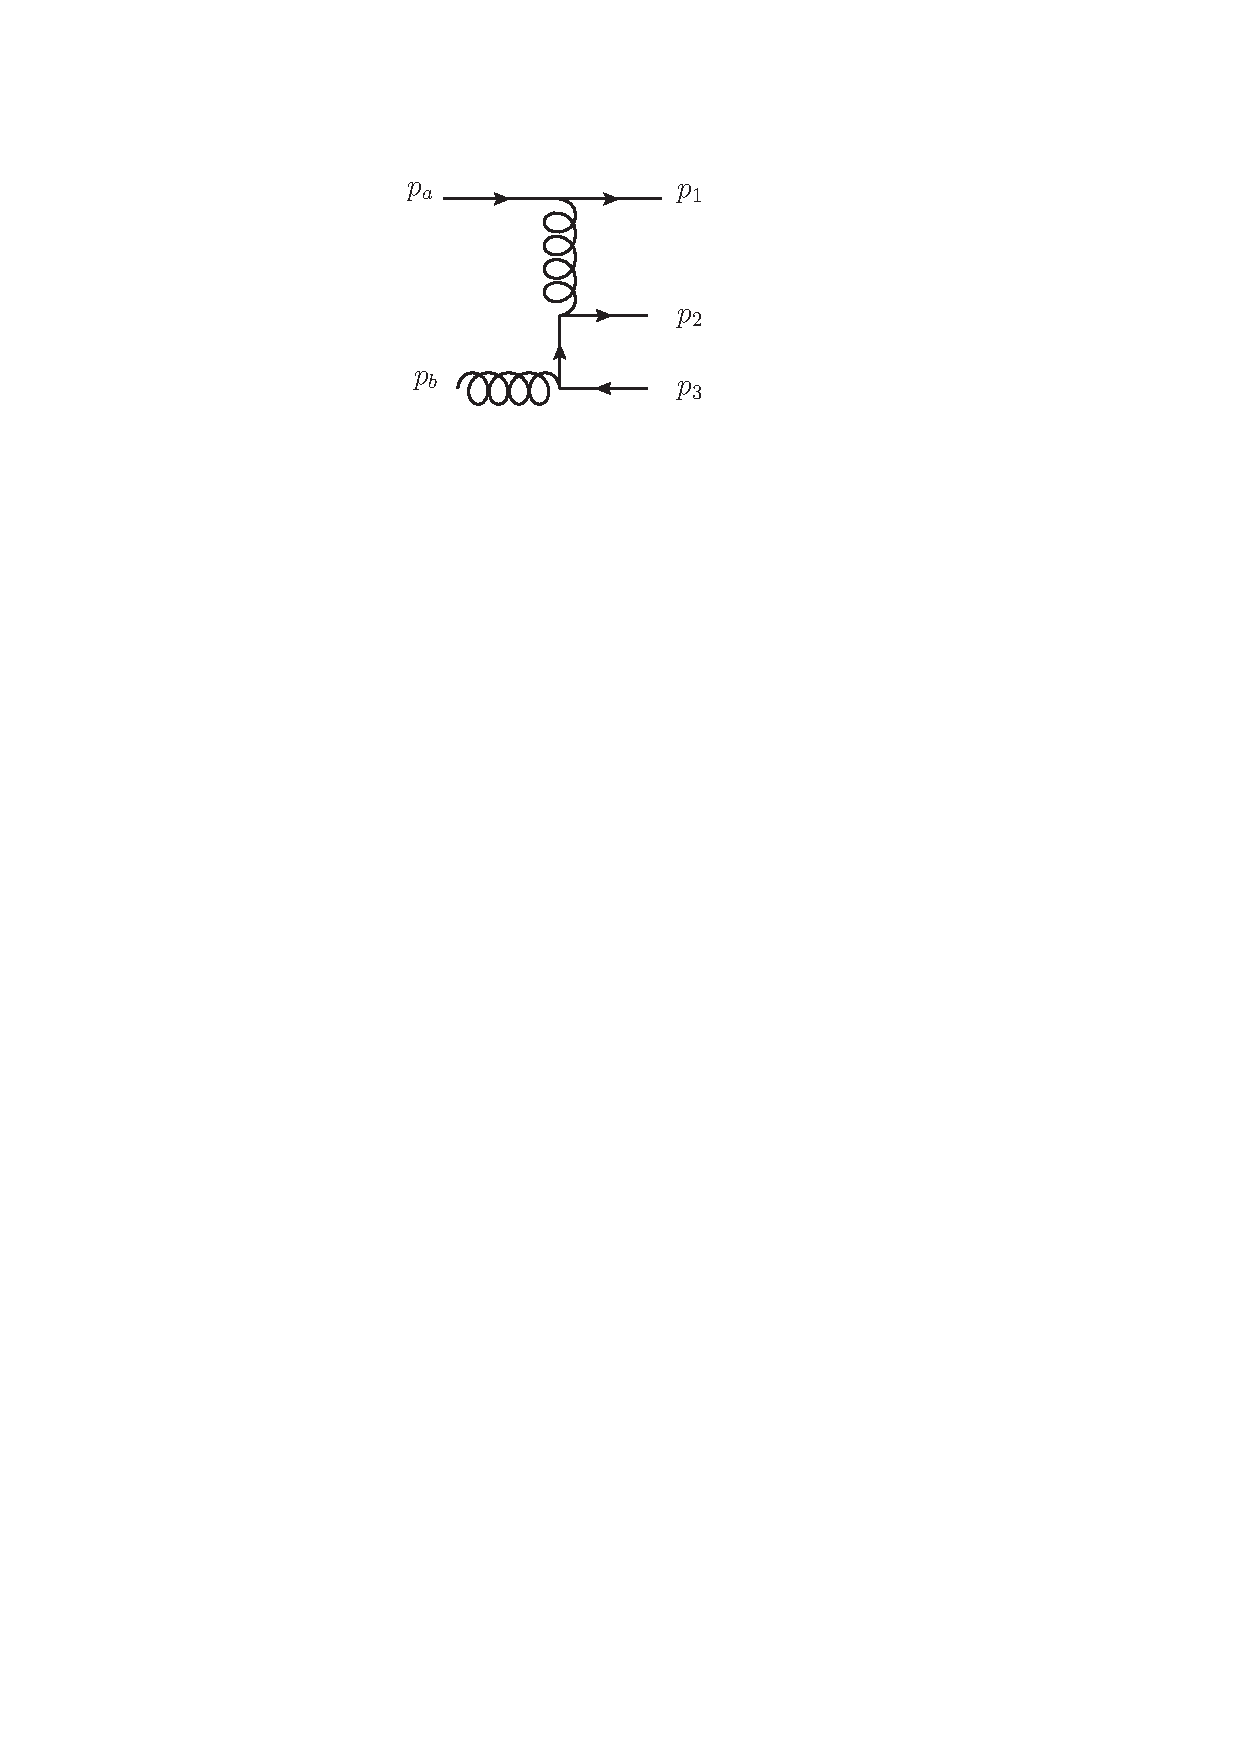
\includegraphics[scale=1]{Images/qg_qQQbar_cross.pdf}} \\
\subfloat{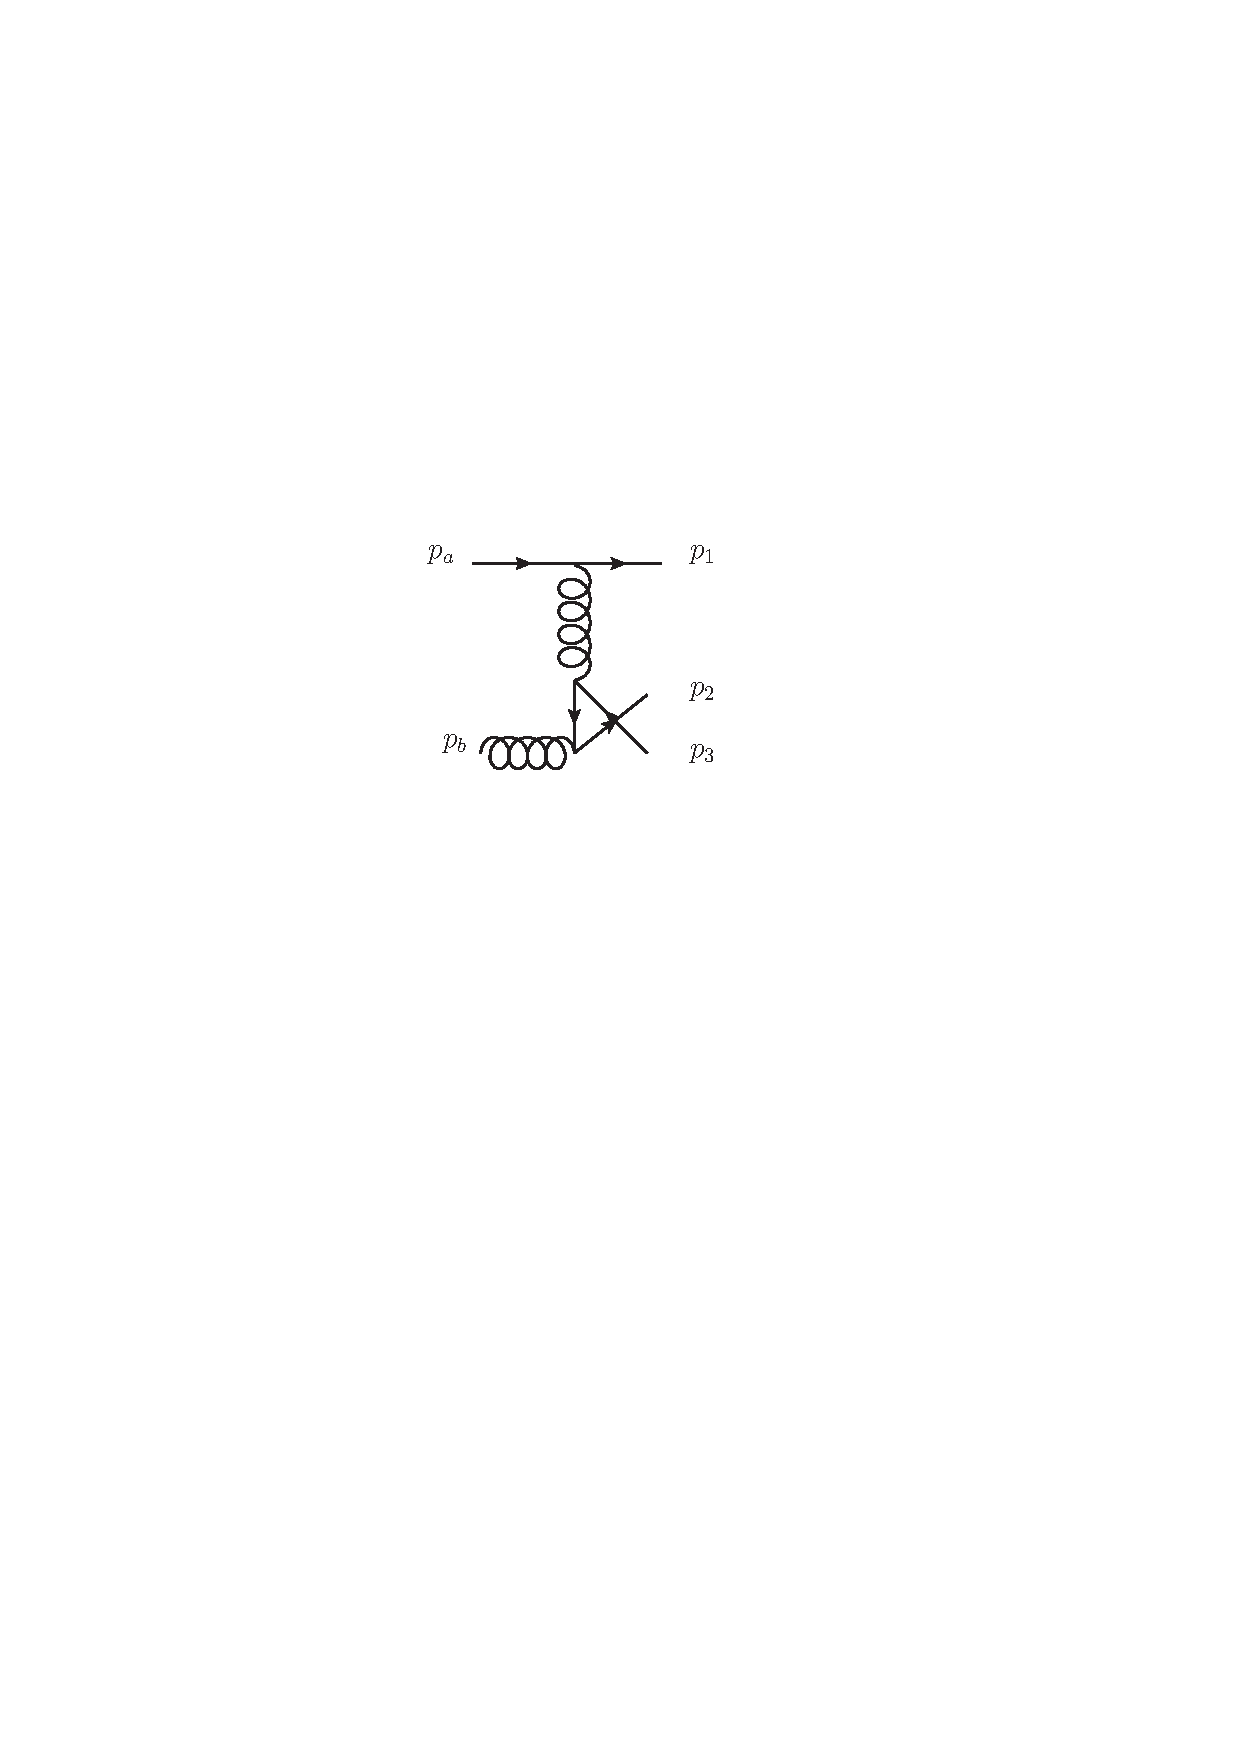
\includegraphics[scale=1]{Images/qg_qQQbar_cross2.pdf}}
\caption{All LO graphs for $qg \to qQ\bar{Q}$.}
\label{fig:qg_qQQ_graphs}
\end{figure}

The technique for this is as follows: we will first study the complete amplitude for $qg \to qQ\bar{Q}$, for which there are five contributing diagrams as shown in figure \ref{fig:qg_qQQ_graphs}. After we have the full LO expression, we will make some approximations based on the High Energy behaviour of the process to bring the entire amplitude into the desired form. During this approximation stage, we must remember to take care to maintain gauge invariance since our final expression will be applied in all of phase space. We remind the reader at this point that, in the massless quark limit, $u^\pm(p) = v^\mp(p)$ and so the notation $\matel{p}{\mu}{k}$ can refer to $\bar{u}_p \gamma^\mu v_k$ or $\bar{u}_p \gamma^\mu u_k$ interchangeably with no practical need to distinguish. 

We will begin with the diagram shown in the top left of figure  \ref{fig:qg_qQQ_graphs} and then proceed from left to right and top to bottom. Using the Feynman rules, we see this contribution is
\begin{equation}
\begin{split}
iM_1 &= \bar{u}_1(-ig_s\gamma^\nu T^g_{1q})\frac{i(\slashed{p}_a+\slashed{p}_b)}{s_{ab}}(-ig_s \gamma^\mu T_{qa}^b)u_a \varepsilon_\mu(p_b) \frac{-i \eta^{\nu \sigma}}{s_{23}} \matel{2}{\sigma}{3} (- i g_s T^g_{23}) \\
&= \frac{i g_s^3 T^g_{1q}T^b_{qa}T^g_{23}}{s_{ab}s_{23}} \left[ \bar{u}_1 \gamma^\nu (\slashed{p}_a + \slashed{p}_b) \gamma^\mu u_a \right] \matel{2}{\nu}{3} \varepsilon_\mu (p_b).
\end{split}
\end{equation}
For the diagram involving a $u$-channel quark propagator, the expression is very similar:
\begin{equation}
iM_2 = \frac{-i g_s^3 T^b_{1q}T^g_{qa}T^g_{23}}{s_{1b}s_{23}} \left[ \bar{u}_1 \gamma^\mu (\slashed{p}_1 - \slashed{p}_b) \gamma^\nu u_a \right] \matel{2}{\nu}{3} \varepsilon_\mu (p_b).
\end{equation}
The next diagram involves a three-gluon vertex and by invoking the Feynman rules we get
\begin{equation}
iM_3 = \left[\bar{u}_1(-i g_s \gamma^\mu T^g_{1a}) u_a \right] \frac{-i \eta_{\mu \nu}}{\hat{t}_1} \left[\bar{u}_2 (-i g_s \gamma^\rho T^{g'}_{23}) v_3 \right] \frac{- i \eta_{\beta \rho}}{s_{23}} (-g_s f^{g g' b})V_{3g}^{\nu  \beta \alpha} \varepsilon_\alpha(p_b),
\end{equation}
where
\begin{equation}
\begin{split}
V_{3g}^{\nu \beta \alpha} &= (q_1+q_2)^\alpha \eta^{\nu \beta} - (q_2+p_b)^\nu \eta^{\beta \alpha} + (p_b-q_1)^\beta \eta^{ \alpha \nu} \\
&= (2p_2 + 2p_3)^\alpha \eta^{\nu \beta} - (2p_b)^\nu \eta^{\beta \alpha} + (2p_b)^\beta \eta^{ \alpha \nu},
\end{split}
\end{equation}
once terms that are zero when contracted with terms outside of the three-gluon vertex are removed. Algebraic manipulation of this expression leads to
\begin{equation}
iM_3 = \frac{-g_s^3 T^g_{1a} T^{g'}_{23} f^{g g' b}}{\hat{t}_1 s_{23}}  \matel{1}{\nu}{a} \matel{2}{\beta}{3} V_{3g}^{\nu \beta \alpha}\epsilon_\alpha(p_b).
\end{equation}
Finally, we have the last two diagrams that involve both a $t$-channel gluon and quark propagator. For the first, we have
\begin{equation}
iM_4 = \left[\bar{u}_1 (-i g_s \gamma^\mu T^g_{1a}) u_a \right] \frac{-i \eta_{\mu \nu}}{\hat{t}_1} \left[\bar{u}_2 (-i g_s \gamma^\nu T^g_{2q}) \frac{-i (\slashed{p}_3 - \slashed{p}_b )}{t_{3b}} (-i g_s \gamma^\rho T^b_{q3})v_3 \right] \varepsilon_\rho (p_b).
\end{equation}
Note the minus sign in the propagator; this is because the Feynman rule for the quark propagator requires that the momentum flows in the same direction as the charge. This can be written as
\begin{equation}
iM_4 = \frac{-i g_s^3 T^g_{1a}T^b_{q3}T^g_{2q}}{\hat{t}_1 t_{3b}} \matel{1}{\nu}{a}\left[\bar{u}_2 \gamma^\nu (\slashed{p}_3 - \slashed{p}_b) \gamma^\rho v_3 \right] \varepsilon_\rho (p_b).
\end{equation}
A similar analysis yields for the last diagram (no minus sign from the fermion propagator this time)
\begin{equation}
iM_5 = \frac{i g_s^3 T^g_{1a}T^b_{2q}T^g_{q3}}{\hat{t}_1 t_{b2}} \matel{1}{\nu}{a}\left[\bar{u}_2 \gamma^\rho (\slashed{p}_2 - \slashed{p}_b) \gamma^\nu v_3 \right] \varepsilon_\rho (p_b).
\end{equation}
We now have expressions that, when summed, will give the exact, LO result for the process $qg \to qQ\bar{Q}$. Now we must approximate in order to factor out the $t$-channel pole. No approximation is required for $M_3, M_4$ or $M_5$ since the $t$-channel pole is immediately explicit. $M_1$ and $M_2$, however, need special attention. The problematic part is the square brackets of, for example, $M_1$, which we can rewrite using the completeness relation:
\begin{equation}
\bar{u}_1 \gamma^\nu (\slashed{p}_a + \slashed{p}_b) \gamma^\mu u_a = \matel{1}{\nu}{a}2 p_a^\mu + \matel{1}{\nu}{b} \matel{b}{\mu}{a},
\end{equation}
where we continue our notation of not assigning a helicity index to the spinor brackets to indicate that the expansion is valid for both negative and positive helicities. The $\nu$ index is contracted with the quark current $\matel{2}{\nu}{3}$. Depending on the helicity choices, the second term after contraction varies either as $\sqrt{s_{b3} s_{12}}$ or $\sqrt{s_{13} s_{b2}}$. Similarly, the first term varies either as $\sqrt{s_{a3} s_{12}}$ or $\sqrt{s_{13} s_{a2}}$. The relative size of these terms is then $\sqrt{s_{b3}/s_{a3}}$ or $\sqrt{s_{b2}/s_{a2}}$. In the High Energy limit, it is clear that both $s_{a3}$ and $s_{a2}$ are large. Also, since we are dealing with the case where the $Q\bar{Q}$ pair is emitted close in rapidity to one end of the chain, we can reasonably assume that $s_{b3}$ and $s_{b2}$ do not have to be large. We can therefore drop the second term with respect to the first and so
\begin{equation}
iM_1 \approx \frac{i g_s^3 T^g_{1q}T^b_{qa}T^g_{23}}{s_{ab}s_{23}} \left[ 2p_a^\mu \matel{1}{\nu}{a} \right] \matel{2}{\nu}{3} \varepsilon_\mu (p_b).
\end{equation}
A similar argument holds for $M_2$ and so
\begin{equation}
iM_2 \approx \frac{-i g_s^3 T^b_{1q}T^g_{qa}T^g_{23}}{s_{1b}s_{23}} \left[ 2p_1^\mu \matel{1}{\nu}{a} \right] \matel{2}{\nu}{3} \varepsilon_\mu (p_b).
\end{equation}
We can now take the limit $p_a \sim p_1$, which allows us to combine these two diagrams by using the colour commutator result
\begin{equation}
(T^g_{1q}T^b_{qa}- T^b_{1q}T^g_{qa})T^g_{23} = i f^{gbc}T^c_{1a}T^g_{23}.
\end{equation}
This is the same colour factor as that of the diagram involving a $t$-channel gluon exchange under the relabelling $g \to c$ and $g' \to g$. Because of this, we will from now on call the result of this $i C_t$. Thus
\begin{equation}
i(M_1 + M_2) \to \frac{- g_s^3 C_t}{s_{ab}s_{23}}2p_a^\mu \matel{1}{\nu}{a} \matel{2}{\nu}{3} \varepsilon_\mu (p_b),
\end{equation}
and so we have now factored out the quark current in all the amplitudes. If we now combine all the amplitudes together, then we obtain
\begin{equation}
\begin{split}
Q^{\mu \nu} &= -\frac{C_1}{t_{b3}} \left(\bar{u}_2 \gamma^\mu (\slashed{p}_3-\slashed{p}_b)\gamma^\nu v_3 \right) + \frac{C_2}{t_{b2}} \left( \bar{u}_2 \gamma^\nu (\slashed{p}_2-\slashed{p}_b) \gamma^\mu v_3 \right) \\
&+ i  \frac{C_t}{s_{23}} \left(\frac{2 \hspace{2pt} p_a^\nu \hspace{2pt} q_1^2}{s_{ab}}  \matel{2}{\mu}{3} + V^{\mu \rho \nu}_{3g}  \matel{2}{\rho}{3} \right),
\end{split}
\end{equation}
where we have relabelled some Lorentz indices to conform with equation \ref{eqn:NLLeqn} and
\begin{subequations}
\begin{align}
C_1 &= T^g_{1a} T^b_{q3}T^g_{2q}, \\
C_2 &= T^g_{1a} T^b_{2q}T^g_{q3}, \\
C_t &= f^{gbc}T^c_{1a}T^g_{23}.
\end{align}
\end{subequations}
We should check at this point that our expression is indeed still gauge invariant after having made these approximations. The simplest way is to make use of the Ward Identity, which implies $Q^{\mu \nu} p_{b, \nu} = 0$ when gauge invariance is satisfied. Explicitly 
\begin{equation}
\begin{split}
Q^{\mu \nu}p_{b, \nu} &= -\frac{C_1}{t_{b3}} \left(\bar{u}_2 \gamma^\mu \slashed{p}_3 \slashed{p}_b v_3 \right) + \frac{C_2}{t_{b2}} \left( \bar{u}_2 \slashed{p}_b \slashed{p}_2 \gamma^\mu v_3 \right) + i  \frac{C_t}{s_{23}} \left(q_1^2  \matel{2}{\mu}{3} + V^{\mu \rho \nu}_{3g}p_{b \nu}  \matel{2}{\rho}{3} \right) \\
&= -\frac{C_1}{t_{b3}} s_{3b} \matel{2}{\mu}{3} + \frac{C_2}{t_{b2}} s_{2b} \matel{2}{\mu}{3} + i \frac{C_t}{s_{23}}(q_1^2 \matel{2}{\mu}{3} + (s_{2b} + s_{3b})\matel{2}{\mu}{3}\\
&-2p_b^\mu p_b^\rho\matel{2}{\rho}{3} + 2p_b^\mu p_b^\rho \matel{2}{\rho}{3}) \\
&= \frac{\matel{2}{\mu}{3}}{s_{23}}(C_1 s_{23} - C_2 s_{23} + i C_t(q_1^2 + (s_{2b} + s_{3b})) \\
&+ i\matel{2}{\rho}{3} \frac{C_t}{s_{23}}(-2p_b^\mu p_b^\rho + 2p_b^\mu p_b^\rho) \\
&= i C_t \frac{\matel{2}{\mu}{3}}{s_{23}}(-s_{23} + (-s_{2b} - s_{3b} + s_{23} + s_{2b} + s_{3b})) \\
&= 0,
\end{split}
\end{equation}
where we have used the result $C_1 - C_2 = -iC_t$. We therefore conclude that the effective vertex is gauge invariant in all of phase space. It may seem, however, that the effective vertex is not truly factorised since there is a clear instance of $p_a$ in the vertex. Because the complete term goes as $p_a^\mu/s_{ab}$, it is actually independent of $p_a$\footnote{An easy way to convince oneself of this is to work in light-cone co-ordinates and see that the $p_a^+$ scale factors out on the top and bottom of the expression.}. We still have freedom to make a gauge choice for our calculations, however, and a good choice will be the gauge where the gluon polarisation vector is orthogonal to $p_a$, so that %\todo{Am I going to change this given I can symmetrise the pa term?}
\begin{equation}
\begin{split}
Q^{\mu \nu}_{gauge} &= -\frac{C_1}{t_{b3}} \left(\bar{u}_2 \gamma^\mu (\slashed{p}_3-\slashed{p}_b)\gamma^\nu v_3 \right) + \frac{C_2}{t_{b2}} \left( \bar{u}_2 \gamma^\nu (\slashed{p}_2-\slashed{p}_b) \gamma^\mu v_3 \right)  \\
&+ i  \frac{C_t}{s_{23}} \left((2p_2+2p_3)^\nu \eta^{\mu \rho} - 2p_b^\mu \eta^{\nu \rho} + 2p_b^\rho \eta^{\nu \mu} \right) \matel{2}{\rho}{3},
\end{split}
\end{equation}
completing our calculation for the basis HEJ amplitude in the case of an extremal $Q \bar{Q}$ process. Since there are only two independent colour factors in this expression we could rewrite the result in terms of $C_1$ and $C_2$ only, but the author is of the opinion that keeping the terms along with their `natural' colour factors like this is more computationally beneficial and easier to understand. One other interesting point to note is that this effective vertex can be shown to be related to the unordered vertex via crossing symmetry. The full calculation of this is shown in Appendix \ref{app:crossing}. 

\subsection{Verifications of the Extremal $Q\bar{Q}$ Vertex}

In order to check the derivation of this vertex, we will explicitly investigate how the amplitudes that contain it behave in the MRK limit. We discussed before that we expect them to be suppressed by the invariant $s_{Q\bar{Q}}$ with respect to the leading FKL configurations at the $|M|^2$ level. Since the FKL amplitudes behaved as $\hat{s}^2$ at the $|M|^2$ level, we should see a systematic suppression of these new amplitudes if we plot $|M|^2/\hat{s}^2$ and furthermore multiplication of $s_{Q \bar{Q}}$ should combat this. In these amplitudes, we have a more complicated colour structure than we did before, since the effective vertex depends on three colour factors (although only two are actually independent, of course). At the $|M|^2$ level, we must deal with this correctly when performing the colour sum. This is done by splitting up the vertex into sub-vertices, each one of which is associated with one colour factor. We choose to represent this as
\begin{equation}
Q^{\mu \nu} = C_1 Q^{\mu \nu}_1 + C_2 Q^{\mu \nu}_2 + C_t Q^{\mu \nu}_t,
\end{equation}
which allows us to calculate the squared amplitude in the following way:
\begin{equation}
\begin{split}
|M_{qg \to qQ\bar{Q}}|^2 &\sim \frac{1}{24} \bigg(|C_1|^2 Q_1\cdot Q_1^\dagger + |C_2|^2 Q_2 \cdot Q_2^\dagger + |C_t|^2 Q_t \cdot Q_t^\dagger \\
&+ 2 Re(C_1 C_2^\dagger Q_1 \cdot Q_2^{\dagger}) + 2 Re(C_1 C_t^\dagger Q_2 \cdot Q_t^\dagger) + 2 Re(C_2 C_t^\dagger Q_2 \cdot Q_t^\dagger) \bigg),
\end{split}
\end{equation}
where the pre-factor comes from the colour averaging and the colour sum can be explicitly performed. The helicity sum is also performed explicitly and the average brings about a further factor of $1/4$. In order to check how our matrix element performs against the full leading order result (taken from MadGraph), we plot the value of $|M|^2/\hat{s}^2$ through a slice of phase space. The momenta are chosen such that
\begin{equation}
\begin{split}
p_1 & = (40 \cosh(\Delta), 0, 40, 40 \sinh(\Delta)), \\
p_2 & = (40 \sqrt{2}, 40 , -40, 0), \\
p_3 & = (40 \cosh(-\Delta), -40, 0, 40 \sinh(-\Delta)), 
\end{split}
\end{equation}
where $\Delta$ is the rapidity of the extremal jets. Therefore, increasing $\Delta$ corresponds to approaching the high energy limit. The results are plotted in figure \ref{fig:qg_qqqx}. We see that the two calculations follow each other very closely and we also see the suppression at large $\Delta$ as we expect. In figure \ref{fig:qg_qqqx_sqqx}, we multiply this result by $s_{Q \bar{Q}}$ and see that the results tend to a finite constant. Hence, the amplitude is behaving how Regge theory predicts.

\begin{figure}[H]
\centering
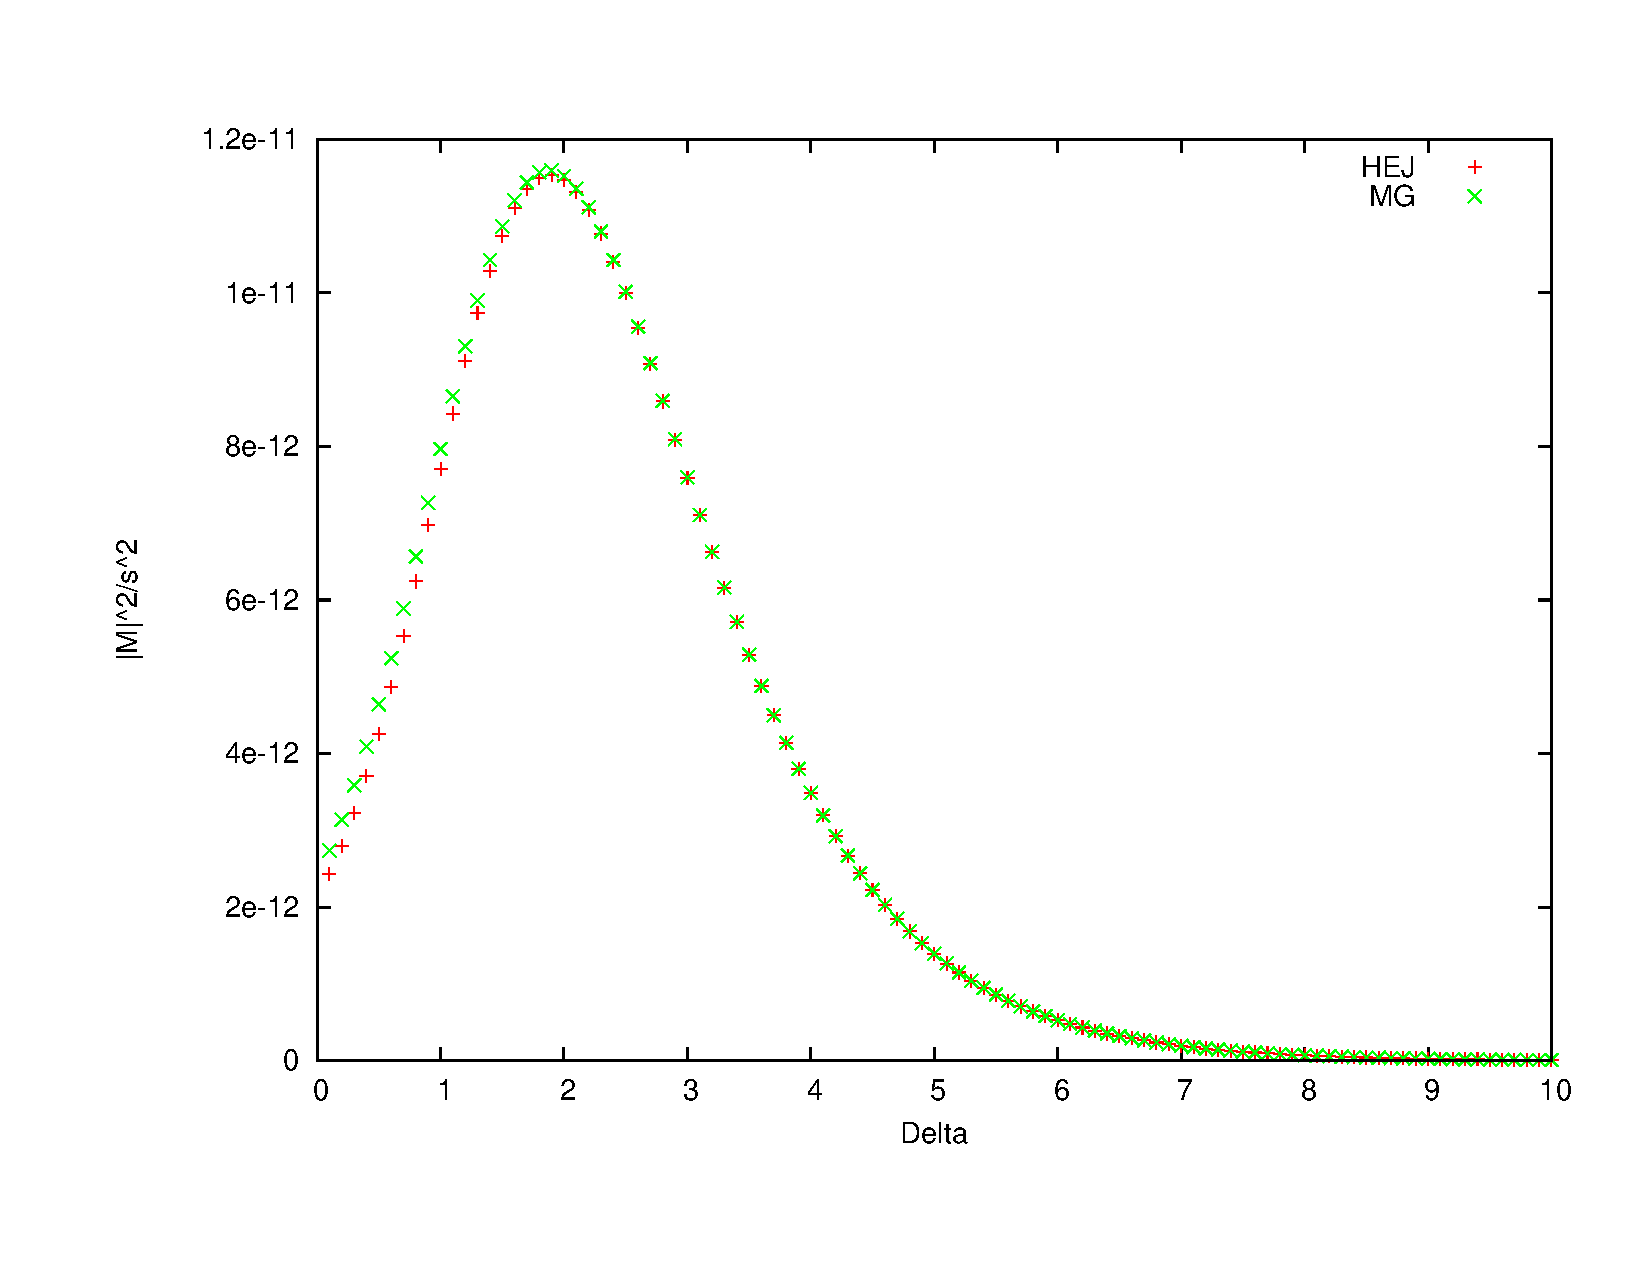
\includegraphics[scale= 0.45]{Images/qg_qqqx.pdf}
\caption{Effective vertex approach to the $qg \to qQ\bar{Q}$ amplitude (red) compared to the full LO (green).}
\label{fig:qg_qqqx}
\end{figure}

\begin{figure}[H]
\centering
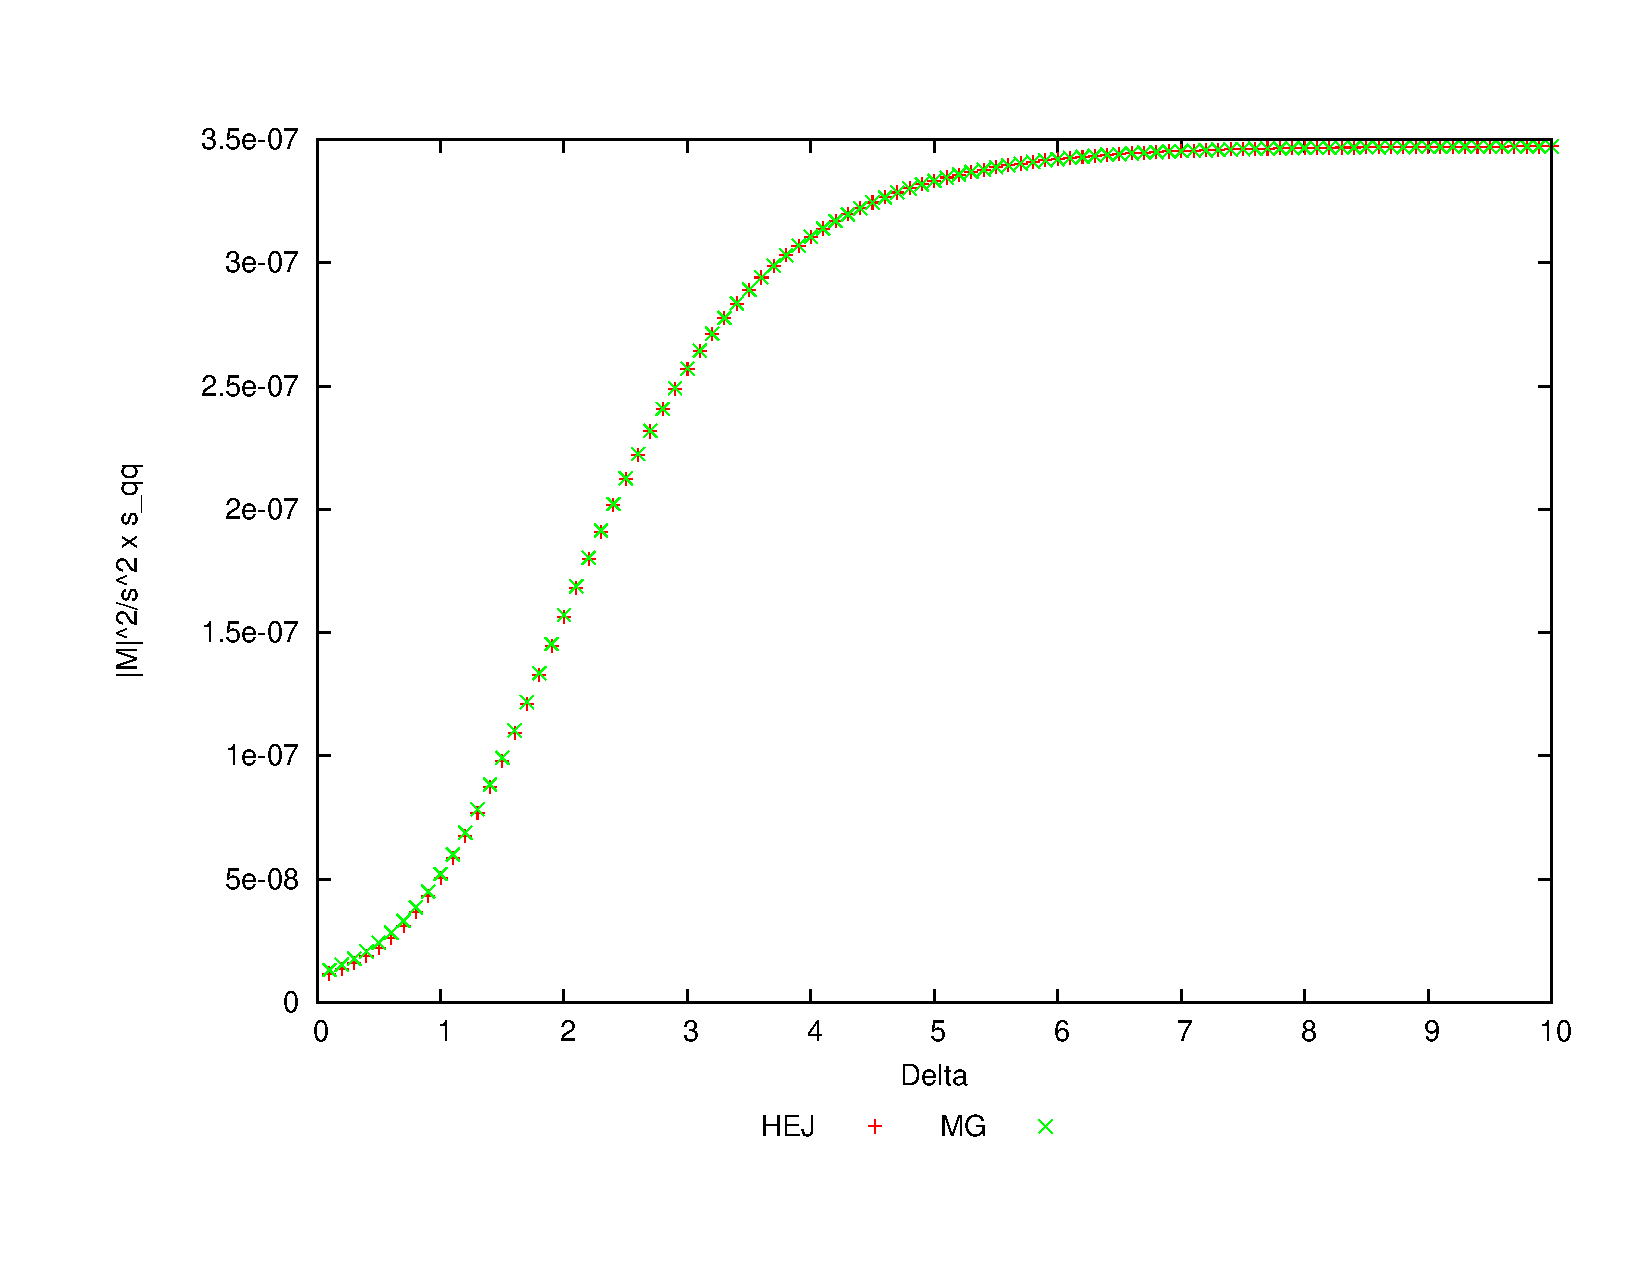
\includegraphics[scale=0.45]{Images/qg_qQQx_sqqx.pdf}
\caption{Effective vertex approach to the $qg \to qQ\bar{Q}$ amplitude (red) compared to the full LO (green) multiplied by the invariant mass of the quark/anti-quark pair.}
\label{fig:qg_qqqx_sqqx}
\end{figure}

Given these plots, we are satisfied that the `base' amplitude works as expected. To extend it, we need to be able to generalise to an arbitrary incoming state and handle extra gluon emissions. The first of these can be achieved by a simple multiplication of a colour factor at the $|M|^2$ level. Since the amplitude must contain at least one incoming gluon, there is only one extra initial state we can have:
\begin{equation}
|M_{gg \to gQ\bar{Q}}|^2 \sim \frac{\tilde{C}_A}{C_F} |M_{qg \to qQ\bar{Q}}|^2,
\end{equation}
where $\tilde{C}_A$ is as defined in equation \ref{eqn:CAM}. We plot this result (multiplied by $s_{Q\bar{Q}}$) along with the full leading order in figure \ref{fig:gg_qqq}. The difference between the two lines is minimal and the only noticeable difference is in the low $\Delta$ regime, where it should be expected to be different since the approximations valid in the High Energy Limit are less accurate here. 

\begin{figure}[t]
\centering
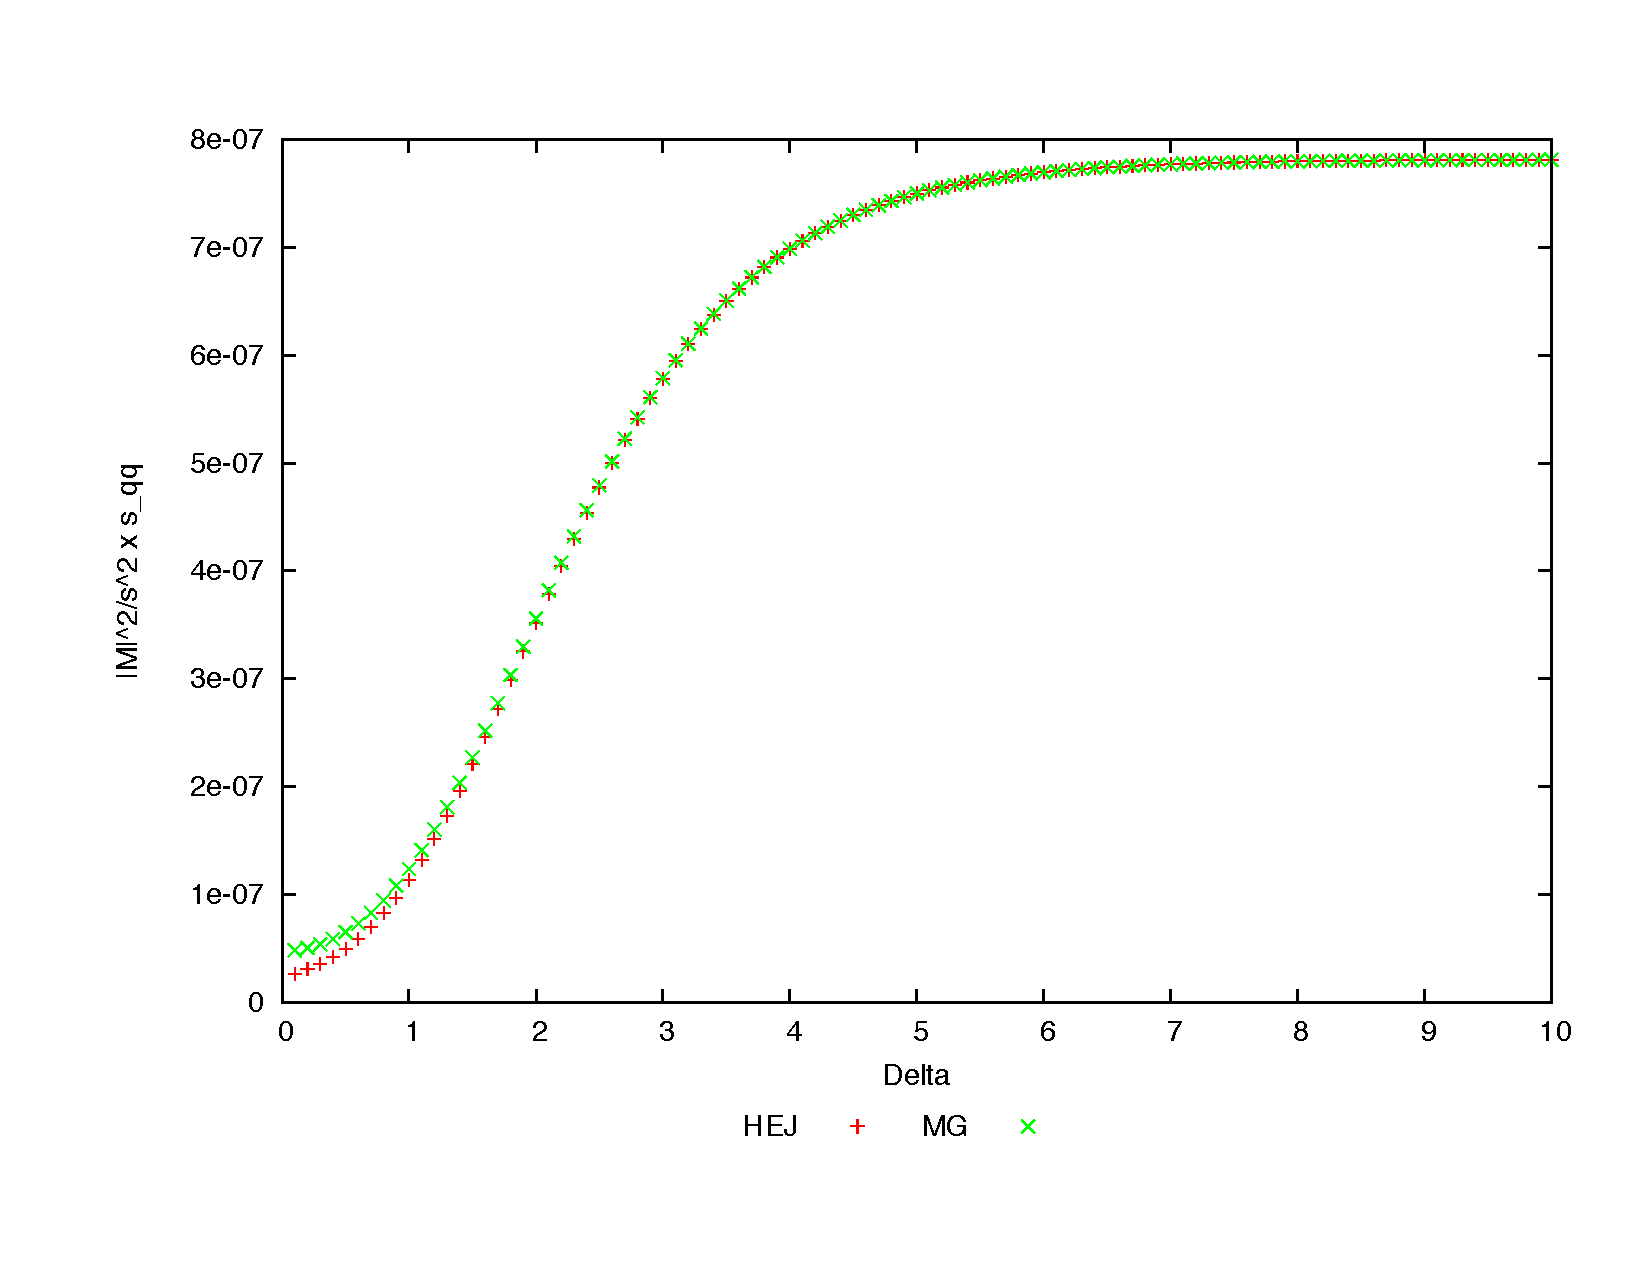
\includegraphics[scale=0.45]{Images/gg_gQQx_sqqx_simplecf.pdf}
\caption{Effective vertex approach to the $gg \to gQ\bar{Q}$ amplitude (red) compared to the full LO (green) multiplied by the invariant mass of the quark/anti-quark pair.}
\label{fig:gg_qqq}
\end{figure}

We then move on to discussing how extra gluon emissions are added to the amplitude. Because of the factorisation properties of the High Energy Limit, so long as we assume the extra gluon emissions are far away in rapidity from the partons already in the amplitude, we can simply insert a Lipatov vertex (defined in equation \ref{eqn:lipatov}), along with a colour factor, and then divide by additional $t$-channel poles that will appear. This yields simply
\begin{equation}
|M_{qg \to q...Q\bar{Q}}|^2 \sim |M_{qg \to qQ\bar{Q}}|^2 \times \prod_{i=1}^{n-3}  C_A \left(\frac{-V(q_i,q_{i+1}) \cdot V(q_i,q_{i+1})}{q_i^2} \right),
\end{equation}
and once more we plot this result against the full LO calculation in figure \ref{fig:qg_qqq_emis} and show that the agreement is still reasonable. 

\begin{figure}[H]
\centering
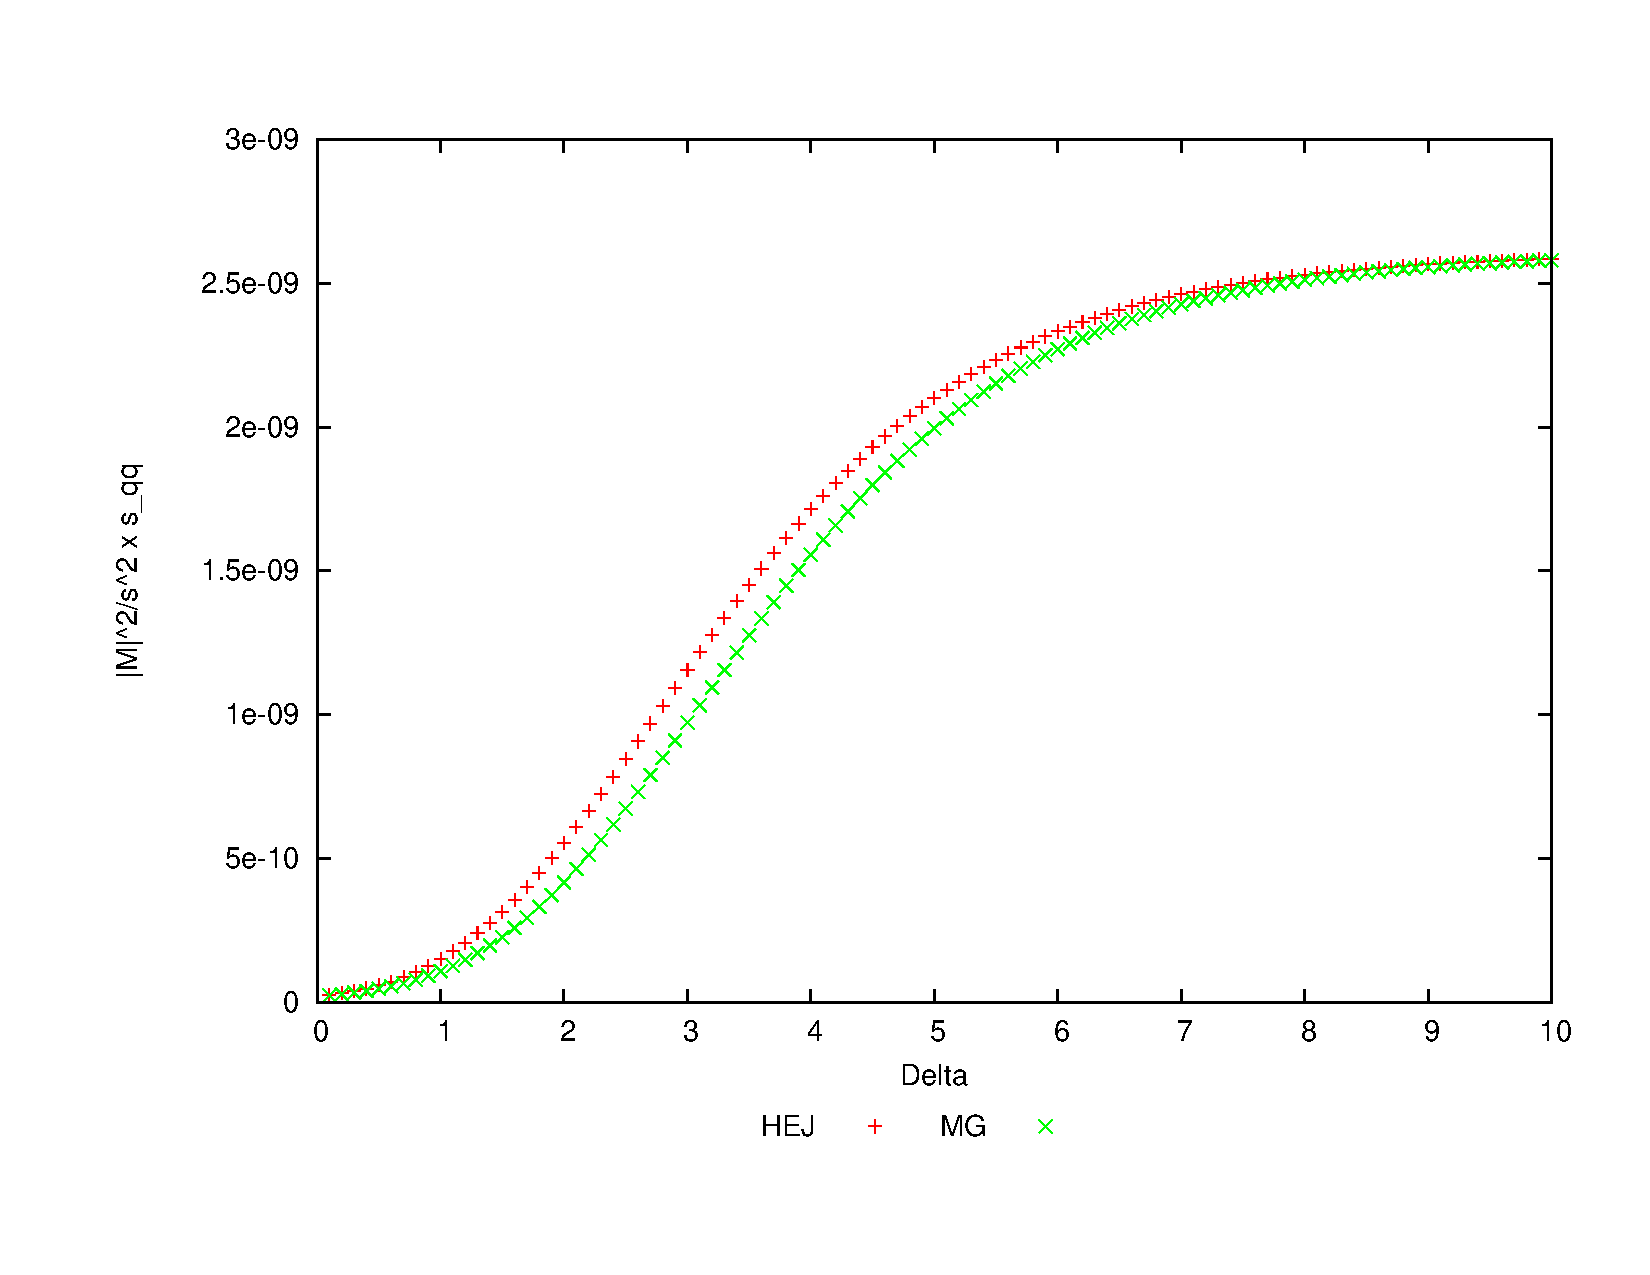
\includegraphics[scale=0.45]{Images/qg_qgQQx_sqq.pdf}
\caption{Effective vertex approach to the $qg \to qgQ\bar{Q}$ amplitude (red) compared to the full LO (green) multiplied by the invariant mass of the quark/anti-quark pair.}
\label{fig:qg_qqq_emis}
\end{figure}

\subsection{Calculation of $qq' \to qQ\bar{Q}q'$ in the High Energy Limit}

The technique for calculating the amplitude for the central process as shown in figure \ref{fig:central} is precisely the same as the one for the extremal process. In this case, we are searching for an amplitude of the form
\begin{equation}
M_{qq' \to qQ\bar{Q}q'} \sim \frac{\matel{1}{\mu}{a}X^{\mu \nu} \matel{4}{\nu}{b}}{\hat{t}_1 \hat{t}_3}.
\end{equation}
There are a total of 7 diagrams to calculate here, shown in figure \ref{fig:qq_qQQq_graphs}. Once more, we will calculate the diagrams starting with the one in the top left and proceeding left to right. The expression for the first diagram is
\begin{equation}
iM_1 = \frac{- i g_s^4 T^e_{1q}T^g_{qa}T^e_{23}T^g_{4b}}{s_{23} \hat{t}_3} \left[ \bar{u}_1 \gamma^\mu \frac{(\slashed{p}_1+\slashed{p}_2 + \slashed{p}_3)}{(p_1 + p_2 + p_3)^2} \gamma^\rho u_a \right] \left[\bar{u}_2 \gamma_\mu v_3 \right] \left[ \bar{u}_4 \gamma_\rho u_b \right].
\end{equation}
\begin{figure}[t]
\centering
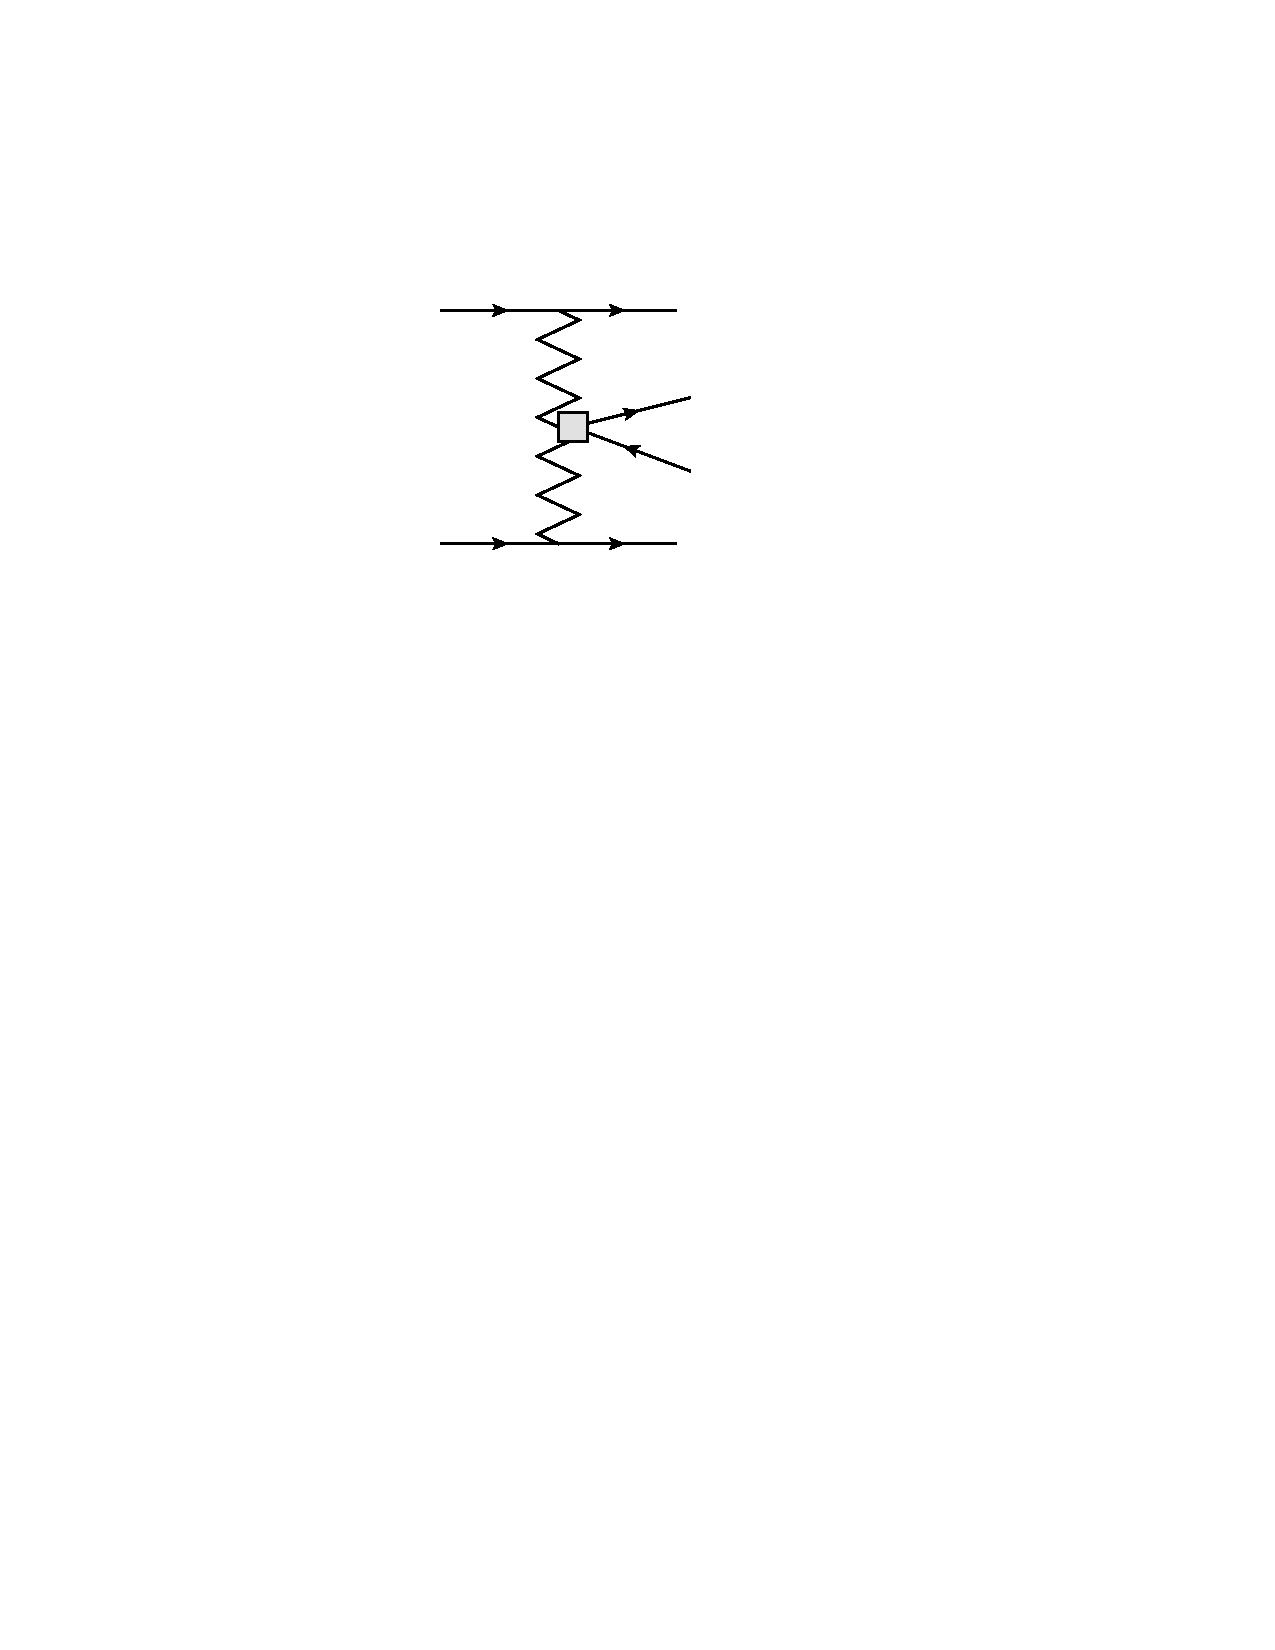
\includegraphics{Images/qq_qqqq_eff.pdf}
\caption{Effective description of $qq' \to qQ\bar{Q}q'$}
\label{fig:central}
\end{figure}
\begin{figure}[t] 
\centering
\subfloat{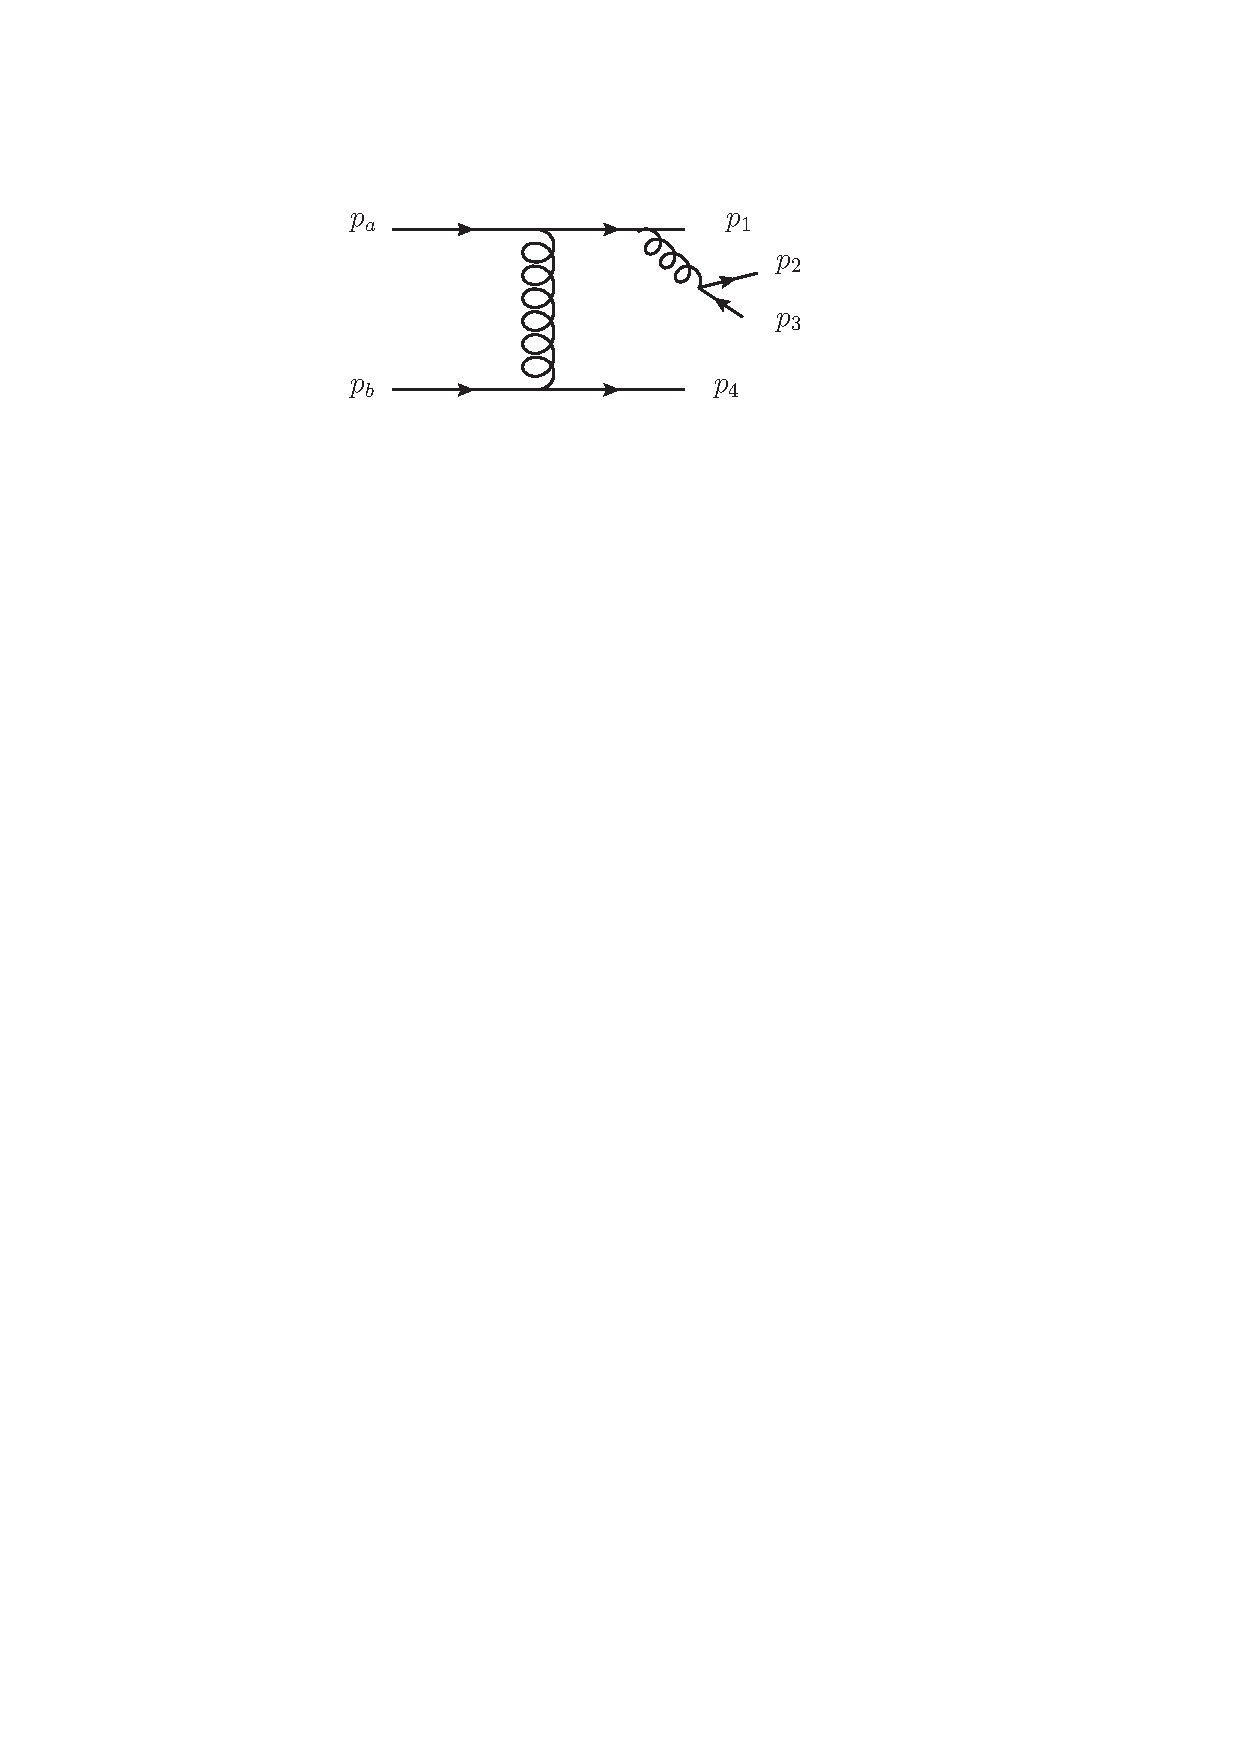
\includegraphics[scale=0.65]{Images/4j_p1_emission.pdf}} 
\subfloat{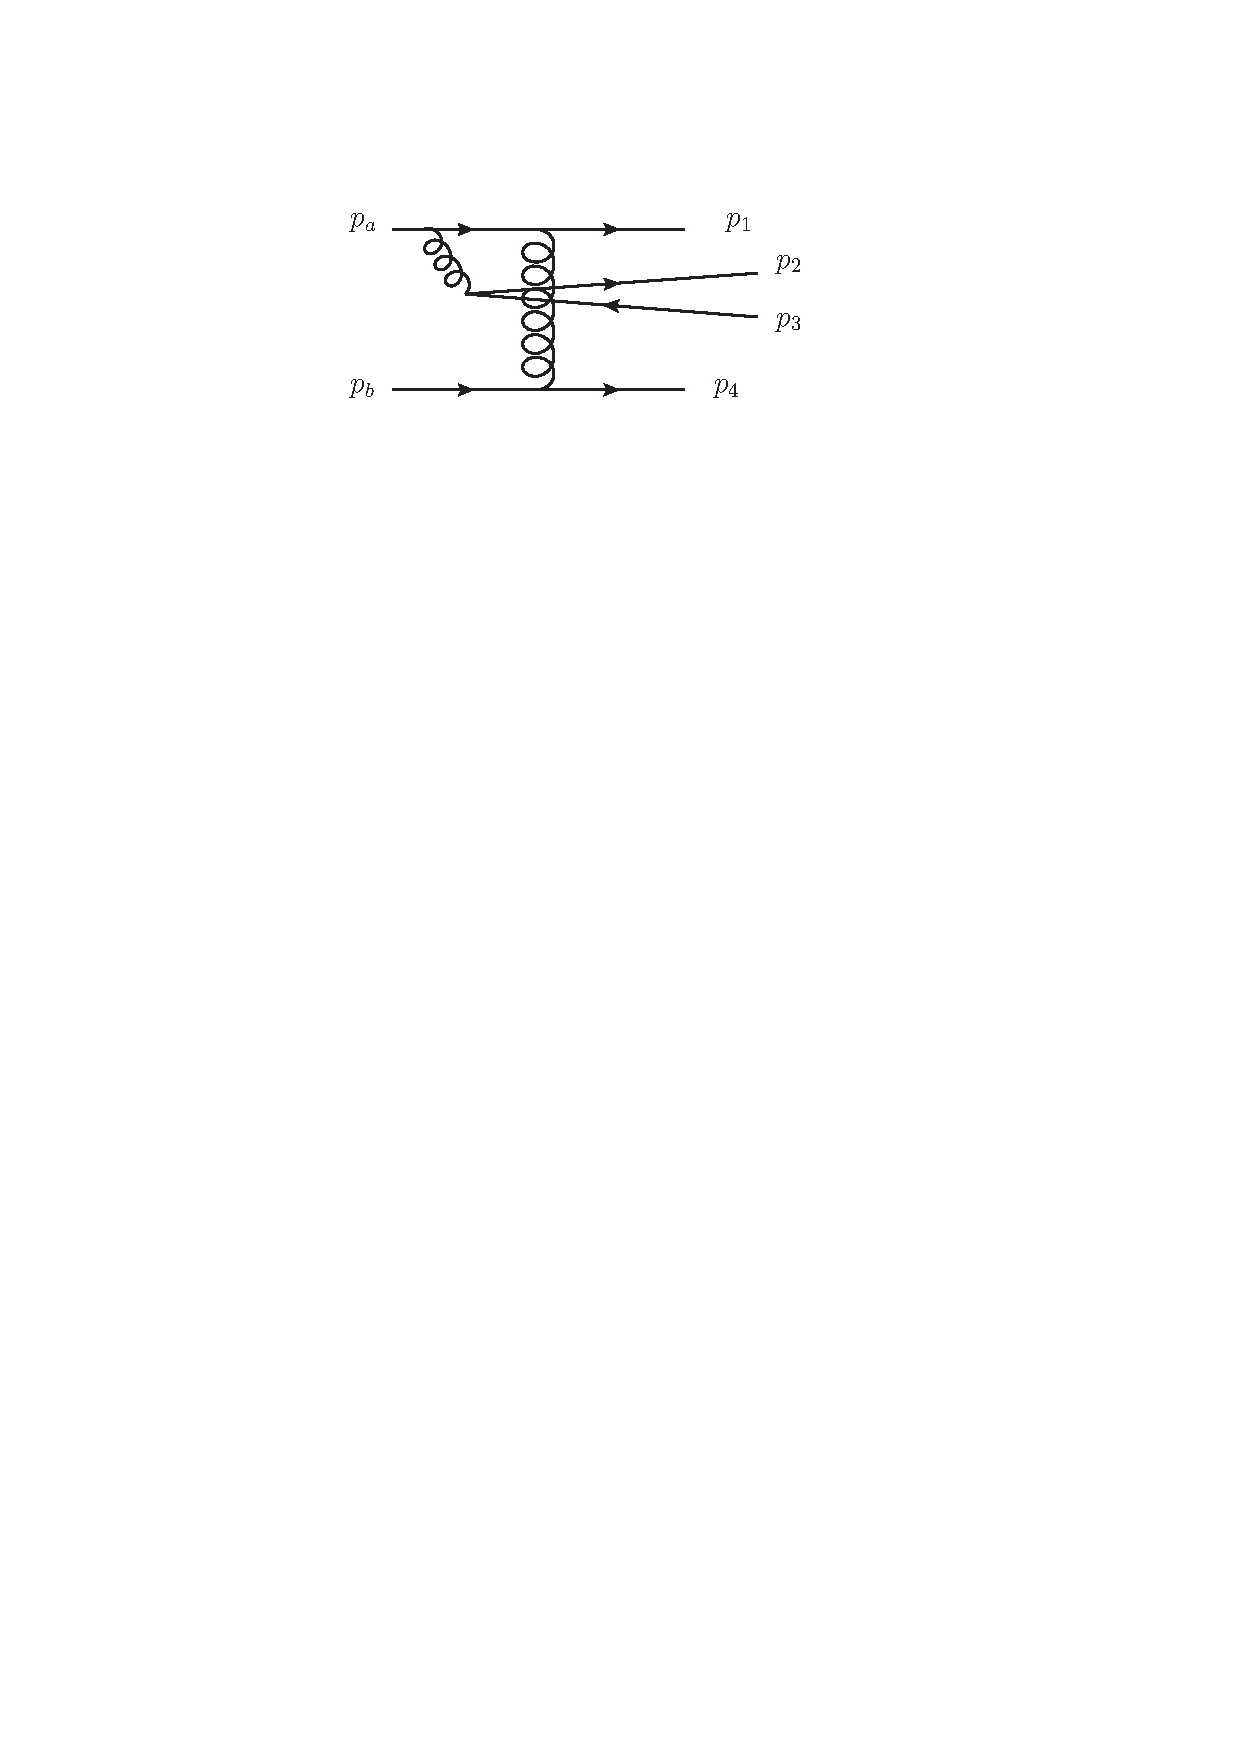
\includegraphics[scale=0.65]{Images/4j_pa_emission.pdf}} 
\subfloat{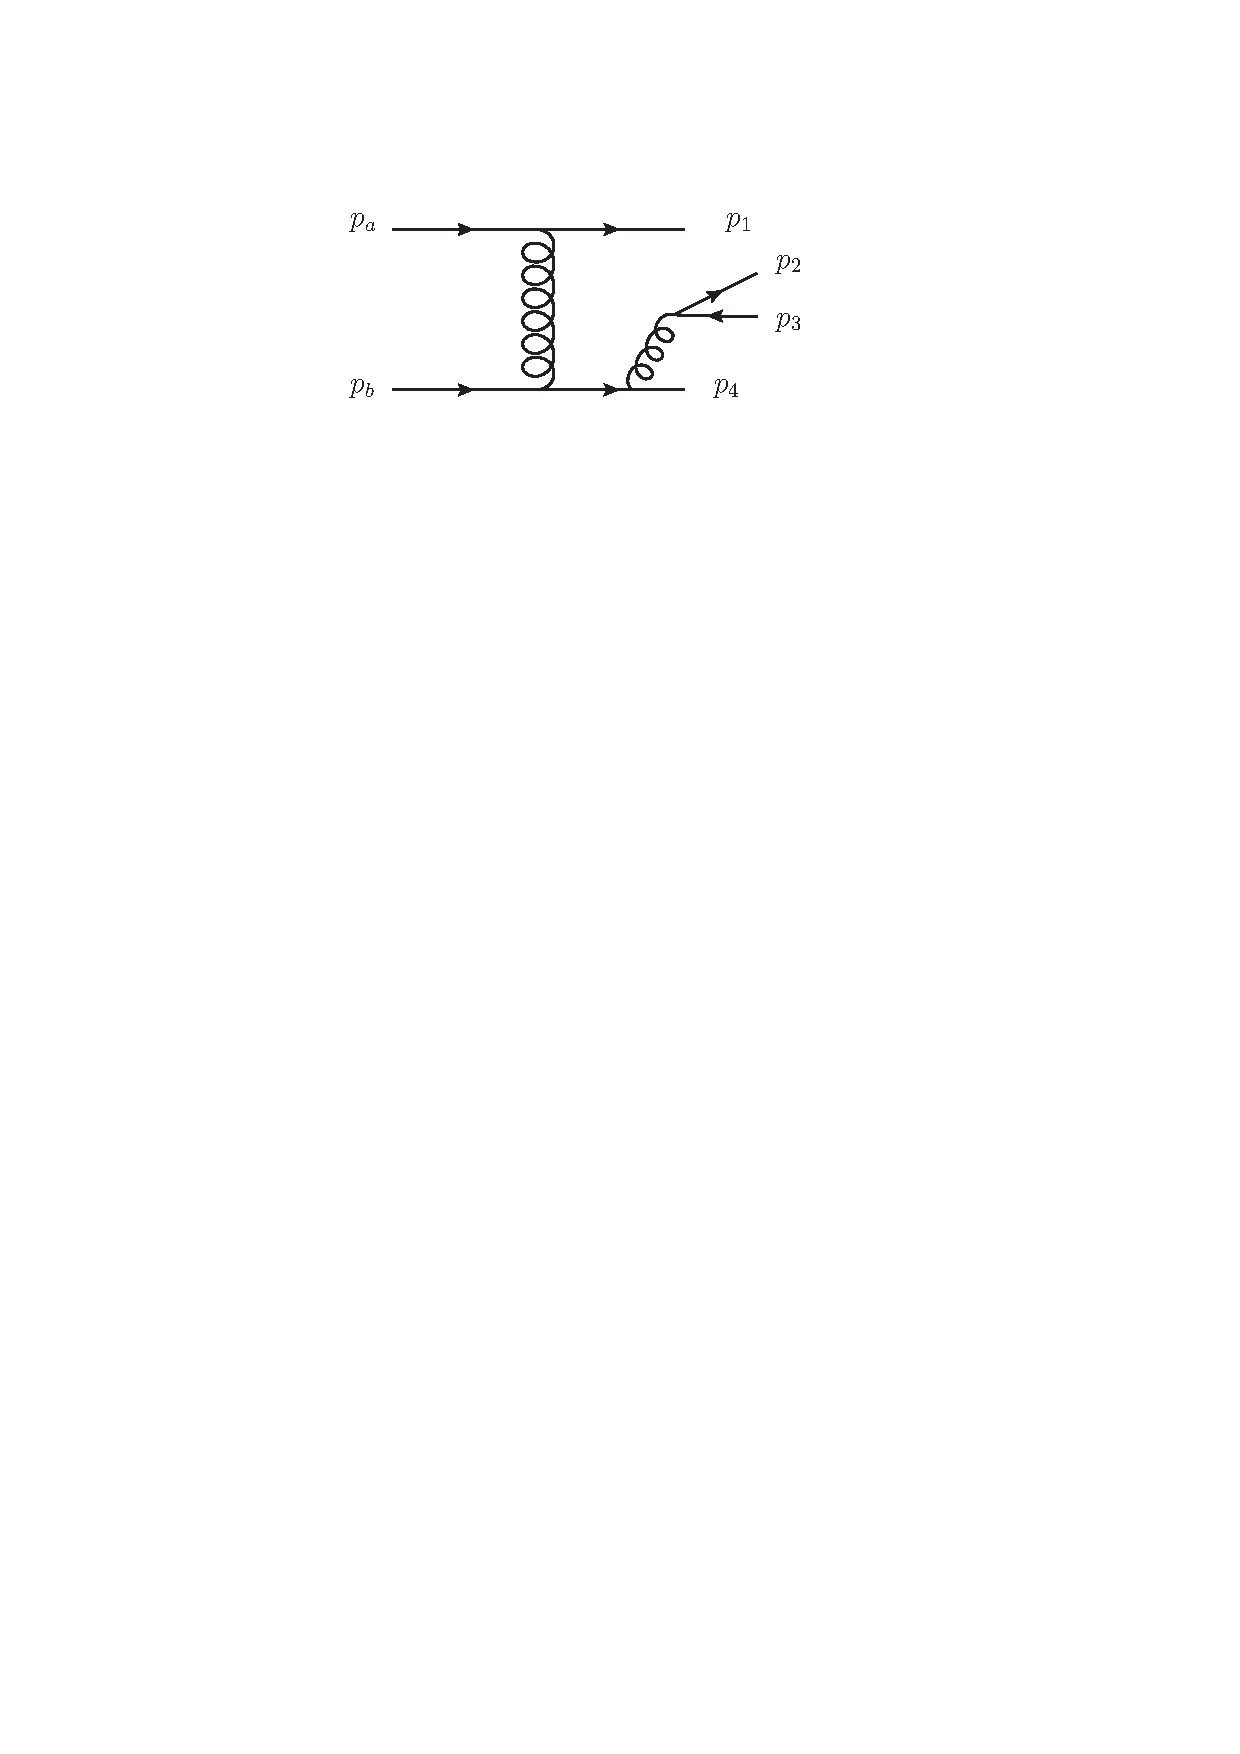
\includegraphics[scale=0.65]{Images/4j_p4_emission.pdf}} \\
\subfloat{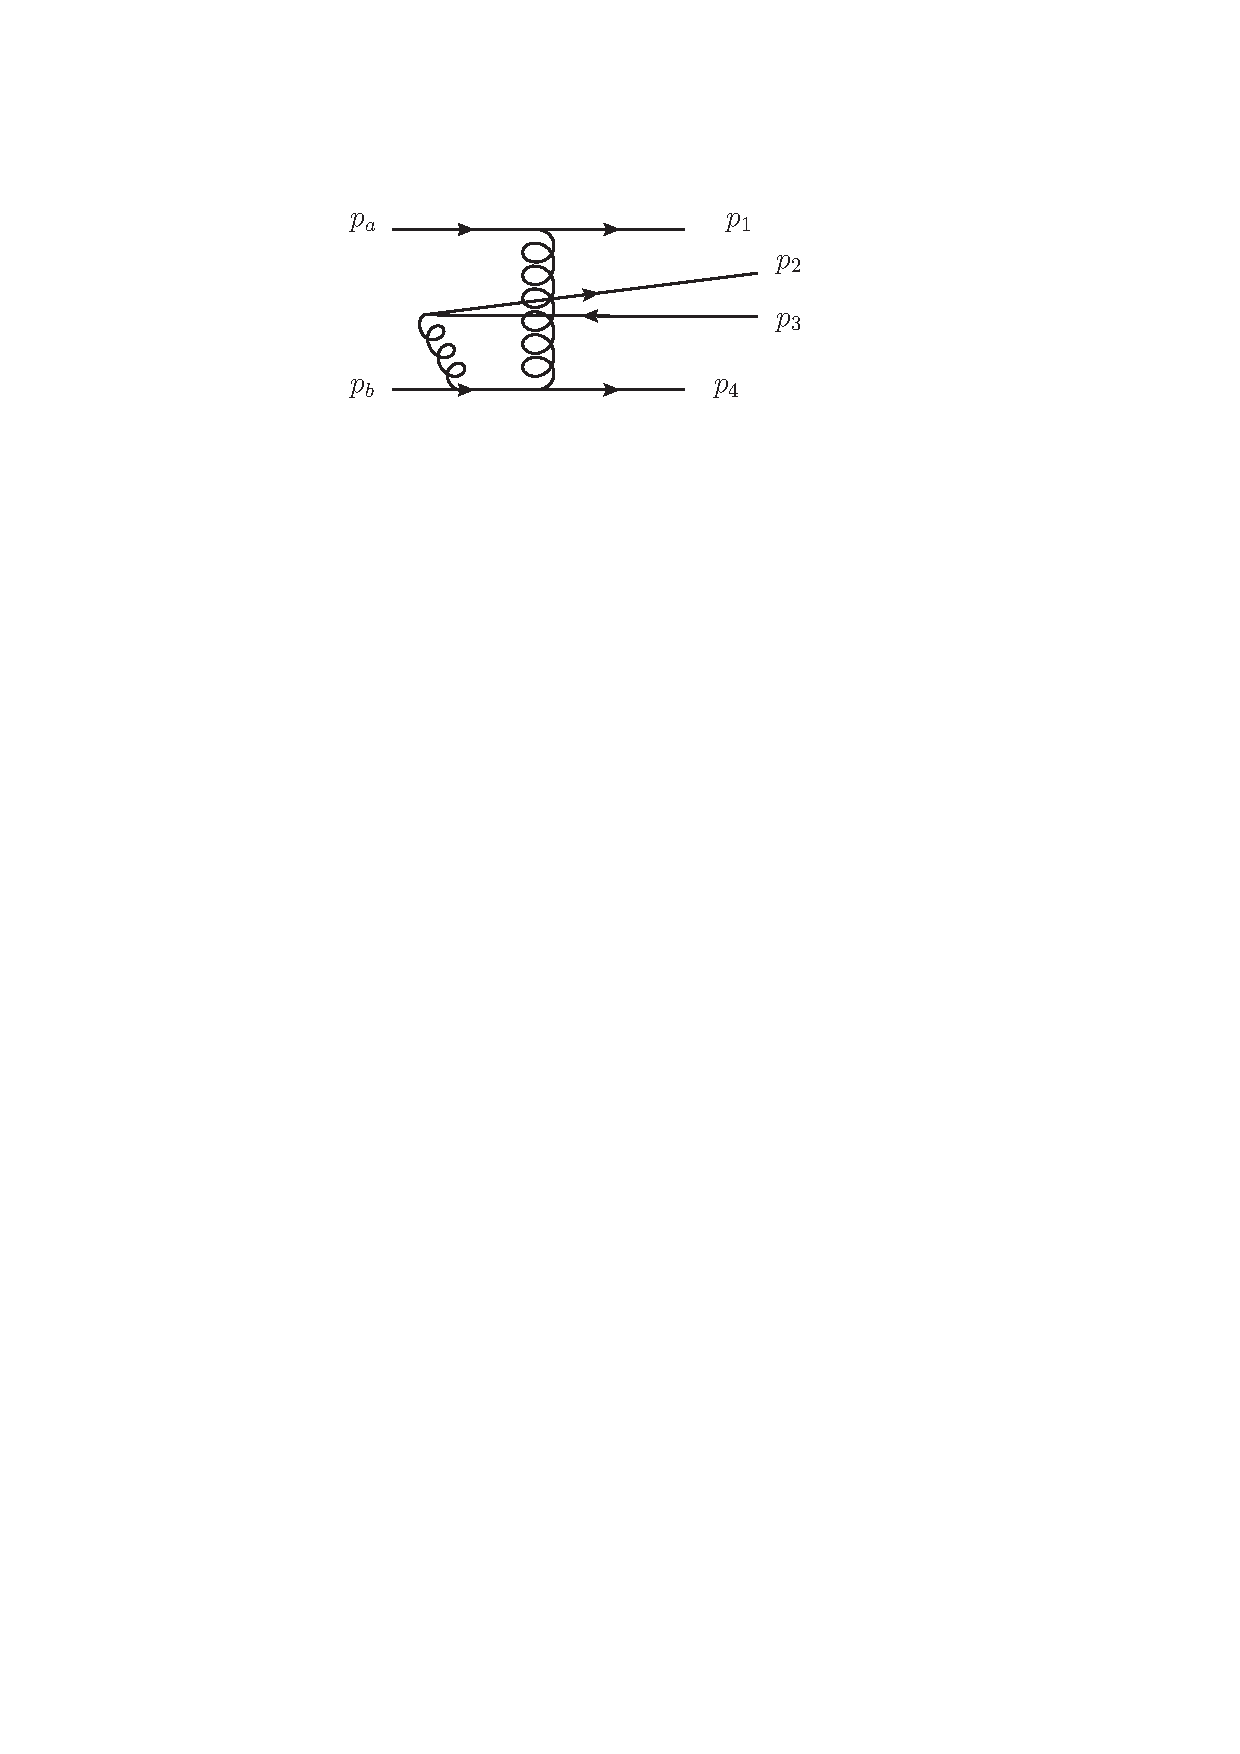
\includegraphics[scale=0.65]{Images/4j_pb_emission.pdf}} 
\subfloat{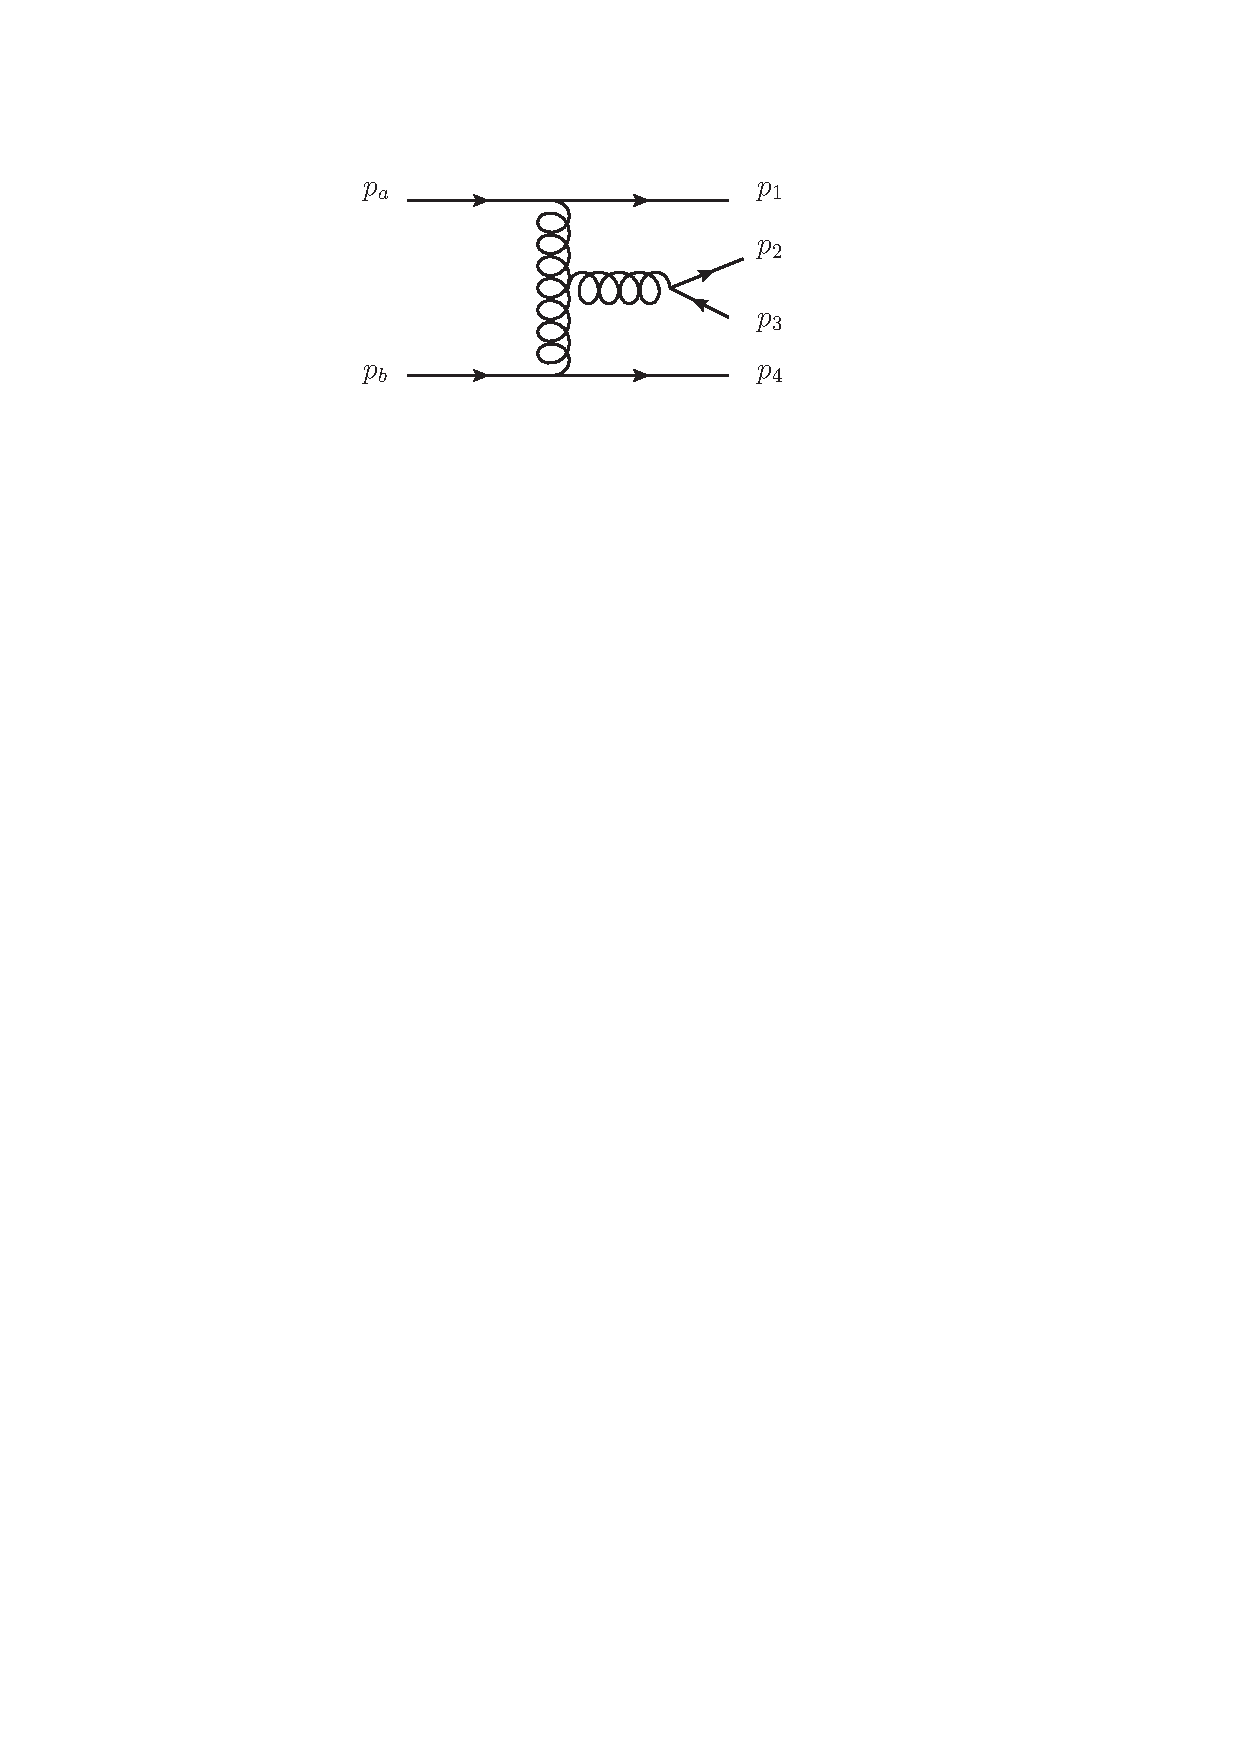
\includegraphics[scale=0.65]{Images/4j_middle_qqg.pdf}}
\subfloat{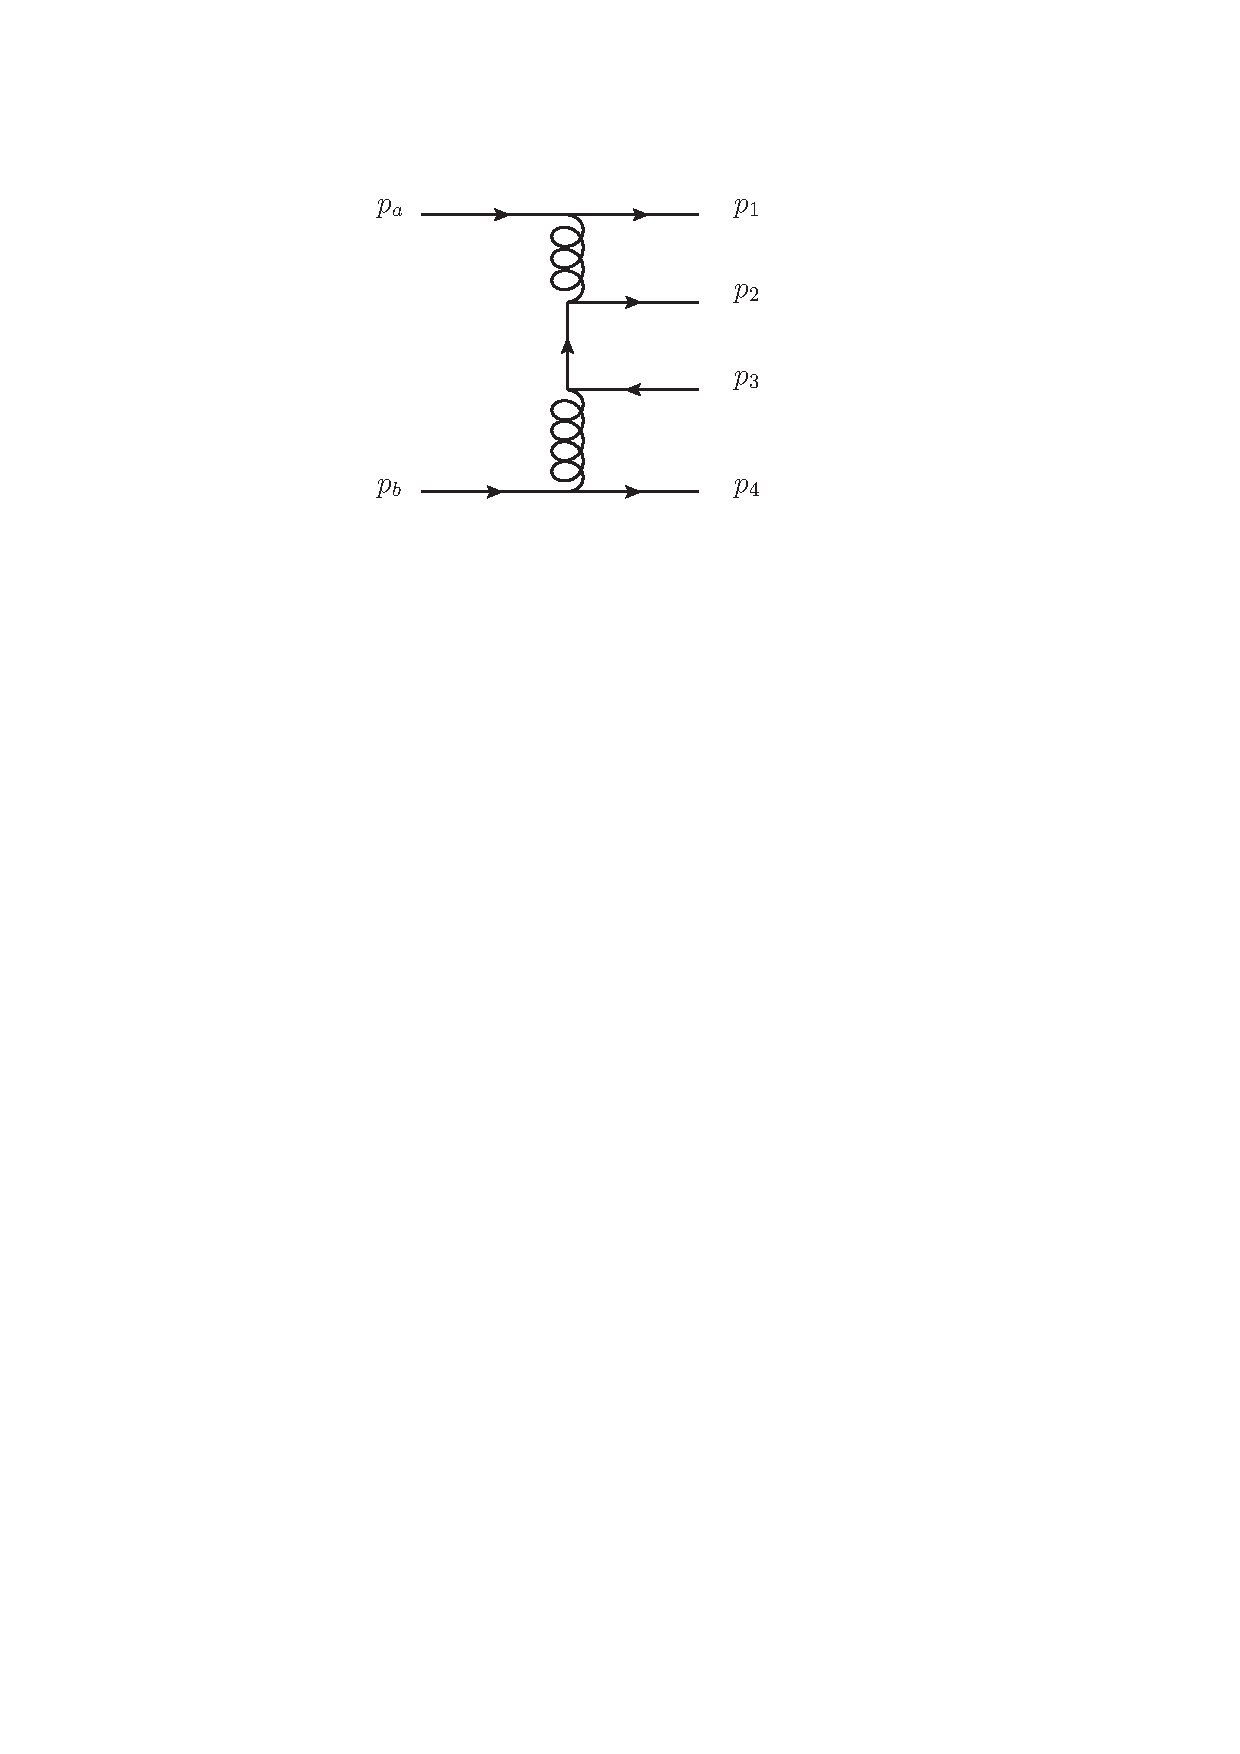
\includegraphics[scale=0.65]{Images/4jet_qprop.pdf}} \\
\subfloat{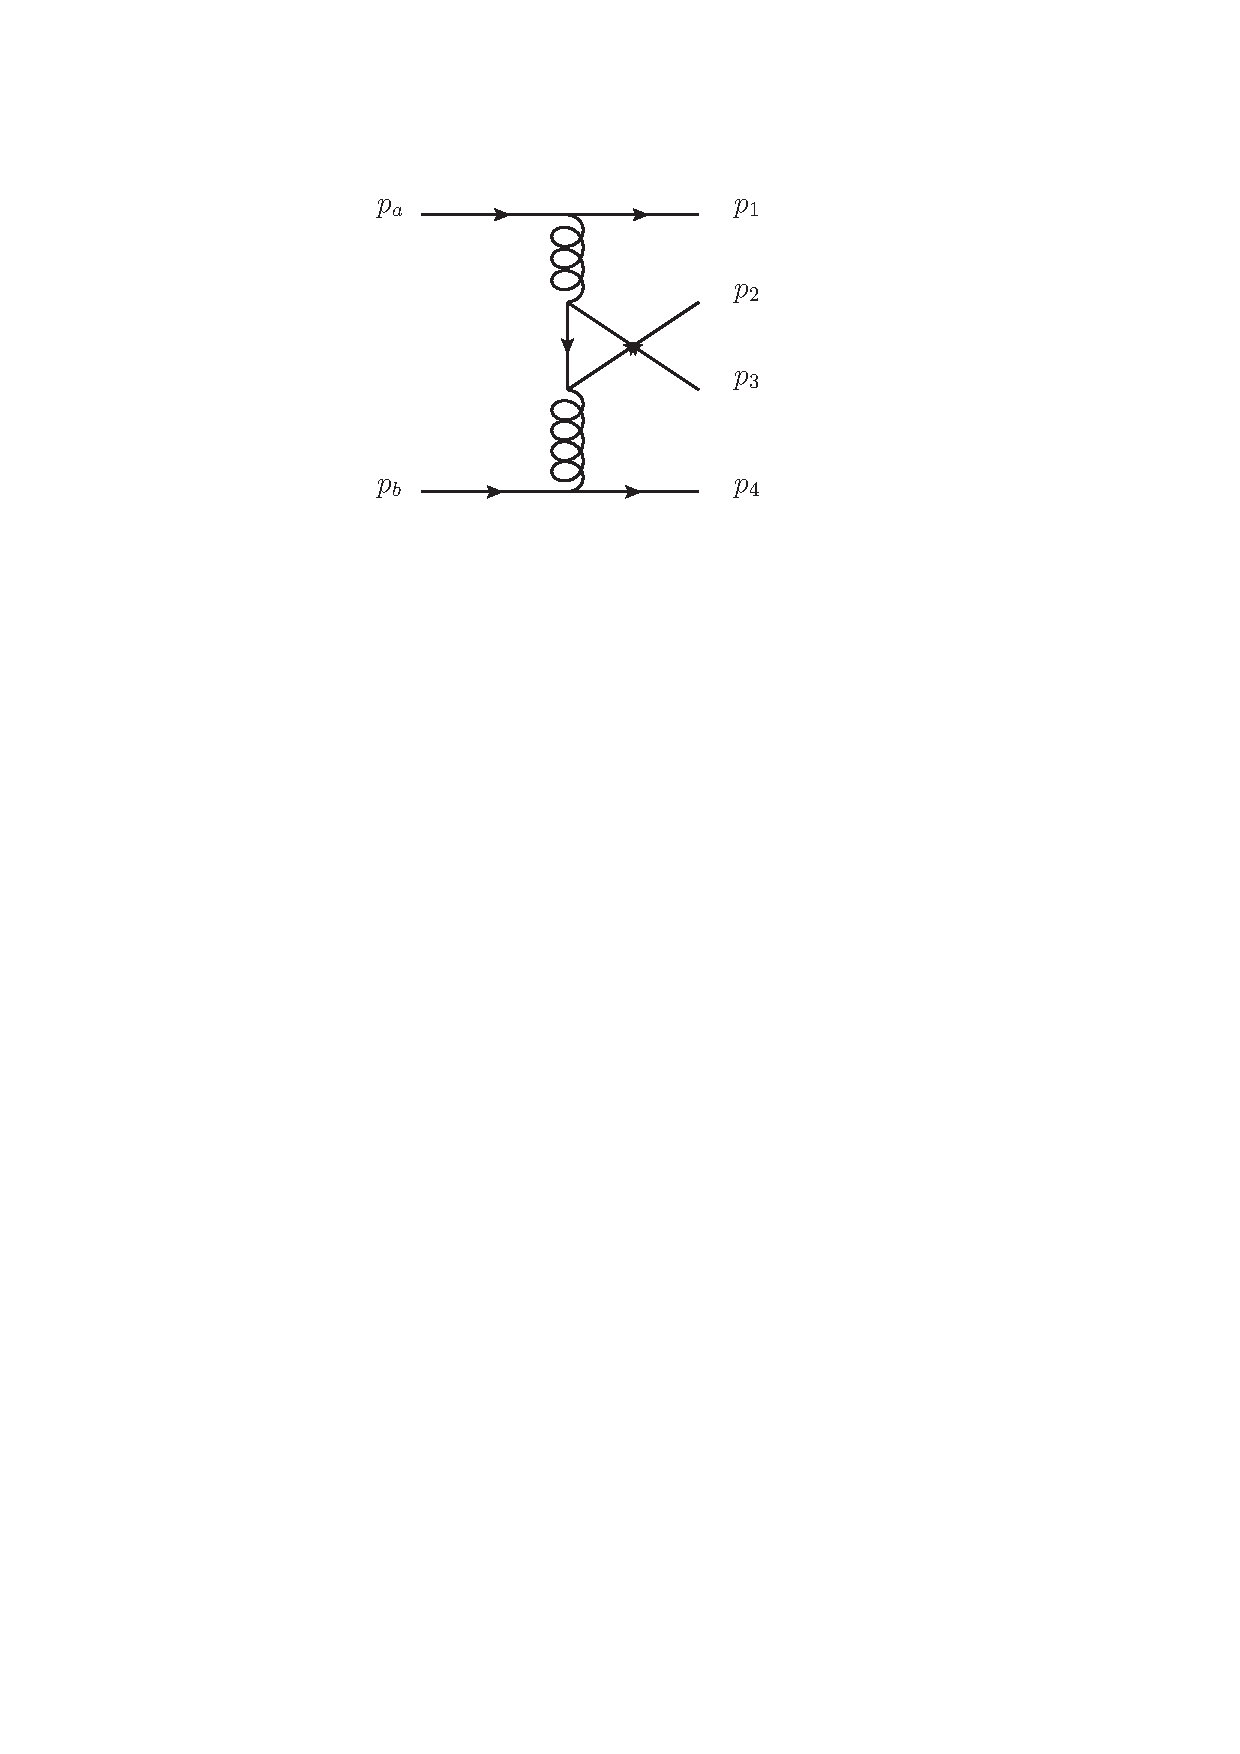
\includegraphics[scale=0.65]{Images/4jet_qprop_crossed.pdf}}
\caption{All LO graphs for $qq' \to qQ\bar{Q}q'$.}
\label{fig:qq_qQQq_graphs}
\end{figure}
It is immediately clear that this diagram will not factorise into our desired form, so we expand the square bracket as a spinor chain again to attempt to make some approximations:
\begin{equation}
\frac{1}{s_{12} + s_{13} + s_{23}} \left(\matel{1}{\mu}{1}\matel{1}{\rho}{a} + \matel{1}{\mu}{2} \matel{2}{\rho}{a} + \matel{1}{\mu}{3} \matel{3}{\rho}{a} \right).
\end{equation}
Depending on the helicities, either the second or third term in this bracket is identically zero when contracted with the quark current $\matel{2}{\mu}{3}$. Once more, we can use a scaling argument to eliminate other terms in this string. The first term contracted with $\matel{2}{\mu}{3}$ will scale as $\sqrt{s_{12} s_{13}}$ regardless of helicity choices. For the other non-zero term, the scaling will be $\sqrt{s_{23} s_{12}}$. We have no requirement that $s_{23}$ be large, but all other invariants \emph{are} large and thus we can approximate the sub-amplitude by keeping the first term only: 
\begin{equation}
iM_1 \approx  \frac{- i g_s^4 T^e_{1q}T^g_{qa}T^e_{23}T^g_{4b}}{s_{23} \hat{t}_3 (s_{12} + s_{13})} \matel{1}{\rho}{a} \matel{4}{\rho}{b} \times 2p_1^\mu \matel{2}{\mu}{3}.
\end{equation} 
The next graph is very similar to the previous and so the calculation proceeds in the same fashion as before. We will then skip to the final expression (having again made the relevant approximation) which is
\begin{equation}
iM_2 \approx \frac{ i g_s^4 T^g_{1q}T^e_{qa}T^e_{23}T^g_{4b}}{s_{23} \hat{t}_3 (s_{a2}+s_{a3})} \matel{1}{\rho}{a} \matel{4}{\rho}{b}\times 2p_a^\mu \matel{2}{\mu}{3}.
\end{equation}    
The next two graphs where the $Q \bar{Q}$ is emitted from the $p_4$ and $p_b$ legs is clearly very similar to the previous two results. Because of this, we simply state the result of the calculation here for these amplitudes which for the $p_4$ leg is
\begin{equation}
iM_3 \approx \frac{-i g_s^4 T^g_{1a} T^e_{4q}T^g_{qb}T^e_{23}}{\hat{t}_1 s_{23}(s_{24}+s_{34})}\matel{1}{\rho}{a} \matel{4}{\rho}{b} \times 2 p_4^\mu \matel{2}{\mu}{3},
\end{equation}
and for the $p_b$ leg is
\begin{equation}
iM_4 \approx \frac{i g_s^4 T^g_{1a} T^g_{4q} T^e_{qb} T^e_{23}}{\hat{t}_1 s_{23}(s_{2b}+s_{3b})} \matel{1}{\rho}{a} \matel{4}{\rho}{b} \times 2 p_b^\mu \matel{2}{\mu}{3}.
\end{equation}
The remaining graphs are already $t$-channel factorised and so we can include them exactly. The next diagram where the $Q \bar{Q}$ emission is from the $t$-channel gluon propagator has the exact expression
\begin{equation}
\begin{split}
iM_5 &= \frac{g_s^4 T^g_{1a} f^{geg'}T^{g'}_{4b}T^e_{23}}{\hat{t}_1 s_{23} \hat{t}_3} \left((q_1 + p_2 + p_3)^\lambda \eta^{\nu \sigma} + (q_3 - p_2 -p_3)^\nu \eta^{\sigma \lambda} - (q_1 + q_3)^\sigma \eta^{\nu \lambda} \right) \\
& \left[\bar{u}_1 \gamma_\nu u_a \right]  \left[\bar{u}_4 \gamma_\lambda u_b \right] \left[\bar{u}_2 \gamma_\sigma v_3 \right],
\end{split}
\end{equation}
where $q_1 = p_a - p_1 = p_4 - p_b + p_3 + p_2 $ and $q_3 = p_4 - p_b = p_a - p_1 - p_2 - p_3$. The final two diagrams both have quark propagators. They have the exact expressions
\begin{equation}
iM_6 = \frac{i g_s^4 T^g_{1a} T^{g}_{2q} T^{g'}_{q3}  T^{g'}_{4b}}{\hat{t}_1 (p_a-p_1-p_2)^2 \hat{t}_3}\left[\bar{u}_1 \gamma^\mu u_a \right] \left[\bar{u}_4 \gamma^\sigma u_b \right] \left[\bar{u}_2 \gamma_\mu(\slashed{p}_a - \slashed{p}_1 -\slashed{p}_2) \gamma_\sigma v_3 \right]
\end{equation}
and
\begin{equation}
iM_7 = \frac{-i g_s^4 T^g_{1a} T^{g'}_{2q} T^{g}_{q3}  T^{g'}_{4b}}{\hat{t}_1 (p_a-p_1-p_3)^2 \hat{t}_3}\left[\bar{u}_1 \gamma^\mu u_a \right] \left[\bar{u}_4 \gamma^\sigma u_b \right] \left[\bar{u}_2 \gamma_\sigma(\slashed{p}_a - \slashed{p}_1 -\slashed{p}_3) \gamma_\mu v_3 \right]
\end{equation}
respectively. Since the High Energy limit here still implies $p_a \sim p_1$ and $p_b \sim p_4$, we can approximately combine both $M_1$ with $M_2$ and $M_3$ with $M_4$. Doing the former yields
\begin{equation}
i(M_1 + M_2) \approx \frac{ C_1 g_s^4}{s_{23} \hat{t}_3 (s_{a2} + s_{a3})} \matel{1}{\rho}{a} \matel{4}{\rho}{b} \times 2 p_a^\sigma \matel{2}{\sigma}{3},
\end{equation} 
where we have defined
\begin{equation}
C_1 = T^e_{1q}T^g_{qa} T^e_{23}T^g_{4b} - T^g_{1q}T^e_{qa}T^e_{23}T^g_{4b} = f^{egc}T^c_{1a}T^e_{23}T^g_{4b},
\end{equation}
and a similar process on $M_3$ and $M_4$ gives
\begin{equation}
i(M_3 + M_4) \to \frac{-C_1 g_s^4}{s_{23}\hat{t}_1 (s_{b2}+s_{b3})} \matel{1}{\rho}{a} \matel{4}{\rho}{b} \times 2 p_b^\sigma \matel{2}{\sigma}{3}. 
\end{equation}
We are then in a position to combine all graphs together and derive our effective vertex $X^{\mu \nu}$:
\begin{equation}
\begin{split}
X^{\mu \nu} &=  \frac{C_1}{s_{23}}\left(\eta^{\mu \nu}\left(2 p_a^\sigma \left( \frac{q_1^2}{s_{a2}+s_{a3}} \right) - 2 p_b^\sigma \left(\frac{q_3^2}{s_{b_2}+s_{b3}} \right) \right)+ V_{3g}^{\mu \nu \sigma} \right)\matel{2}{\sigma}{3} \\
&+ \frac{i C_2}{(p_a-p_1-p_2)^2} X_{qprop}^{\mu \nu} - \frac{i C_3}{(p_a-p_1-p_3)^2} X_{crossed}^{\mu \nu},
\end{split}
\end{equation}
where we have defined the following expressions: %\todo{define the qs}
\begin{subequations}
\begin{align}
V_{3g}^{\mu \nu \sigma} &= (q_1 + p_2 + p_3)^\nu \eta^{\mu \sigma} + (q_3 - p_2 -p_3)^\mu \eta^{\sigma \nu} - (q_1 + q_3)^\sigma \eta^{\mu \nu} \\
C_2 &= T^g_{1a}T^g_{2q}T^{g'}_{q3}T^{g'}_{4b} \\
C_3 &= T^g_{1a}T^{g'}_{2q}T^g_{q3}T^{g'}_{4b} \\
X_{qprop}^{\mu \nu} &= \bar{u}_2 \gamma^\mu (\slashed{q}_1 - \slashed{p}_2)\gamma^\nu v_3 \\
X_{crossed}^{\mu \nu} &=\bar{u}_2 \gamma^\nu (\slashed{q}_1 - \slashed{p}_3)\gamma^\mu v_3.
\end{align}
\end{subequations}
In fact, since we assumed $p_a \sim p_1$ and $p_b \sim p_4$ in deriving this form, we can go one step further and reinstate this symmetry. Such a step is consistent with how we treat the Lipatov vertex and will only affect sub-leading terms. Our final vertex is then
\begin{equation}
%\begin{split}
X^{\mu \nu} = \frac{C_1}{s_{23}} \left(\eta^{\mu \nu} X_{sym}^\sigma + V^{\mu \nu \sigma}_{3g} \right) \matel{2}{\sigma}{3} + \frac{i C_2}{(p_a-p_1-p_2)^2} X^{\mu \nu}_{qprop} - \frac{i C_3}{(p_a-p_1-p_3)^2} X^{\mu \nu}_{crossed},
%\end{split}
\end{equation}
with
\begin{equation}
%\begin{split}
X_{sym}^\sigma = p_a^\sigma \left( \frac{q_1^2}{s_{a2}+s_{a3}} \right) + p_1^\sigma \left( \frac{q_1^2}{s_{12}+s_{13}} \right) 
- p_b^\sigma \left( \frac{q_3^2}{s_{b2}+s_{b3}} \right) - p_4^\sigma \left( \frac{q_3^2}{s_{42}+s_{43}} \right).
%\end{split}
\end{equation}
We have intentionally used the notation of $q^2$ to make it clear that this invariant is formed from the mass of the propagator entering into the effective vertex. Once extra emissions are added, the $t_{ij}$ notation can be misleading. With this, we now have the complete expression for the effective central $Q\bar{Q}$ vertex. Furthermore, we notice again that we can rewrite our colour factors in such a way that the vertex depends only on $C_2$ and $C_3$, but we decide not to for computational ease. 

\subsection{Verifications of the Central $Q\bar{Q}$ Vertex}

As with the previous effective vertex, we take this subsection as an opportunity to check the correctness of our calculation. The calculation is once more practically performed by splitting the effective vertex up into sub-vertices according to the colour factors and explicitly summing the contributions at the $|M|^2$ level. We choose the following parametrisation for the momenta: 
\begin{equation}
\begin{split}
p_1 & = (40 \cosh(\Delta), 0, 40, 40 \sinh(\Delta)), \\
p_2 & = (40 \cosh(\Delta/3), 40, 0, 40 \sinh(\Delta/3)), \\
p_3 & = (40 \cosh(-\Delta/3), 0, -40, 40 \sinh(-\Delta/3)), \\
p_4 & = (40 \cosh(-\Delta), -40, 0, 40 \sinh(-\Delta)). 
\end{split}
\label{eqn:4jetmom}
\end{equation}
The comparison between our amplitude and the full leading order is shown in figure \ref{fig:qq_qqqq}. We see once more the good agreement between the two across the phase space as well as the suppression at large $\Delta$, which figure \ref{fig:qq_qqqq_sqq} shows is again due to $s_{Q \bar{Q}}$. 

\begin{figure}[H]
\centering
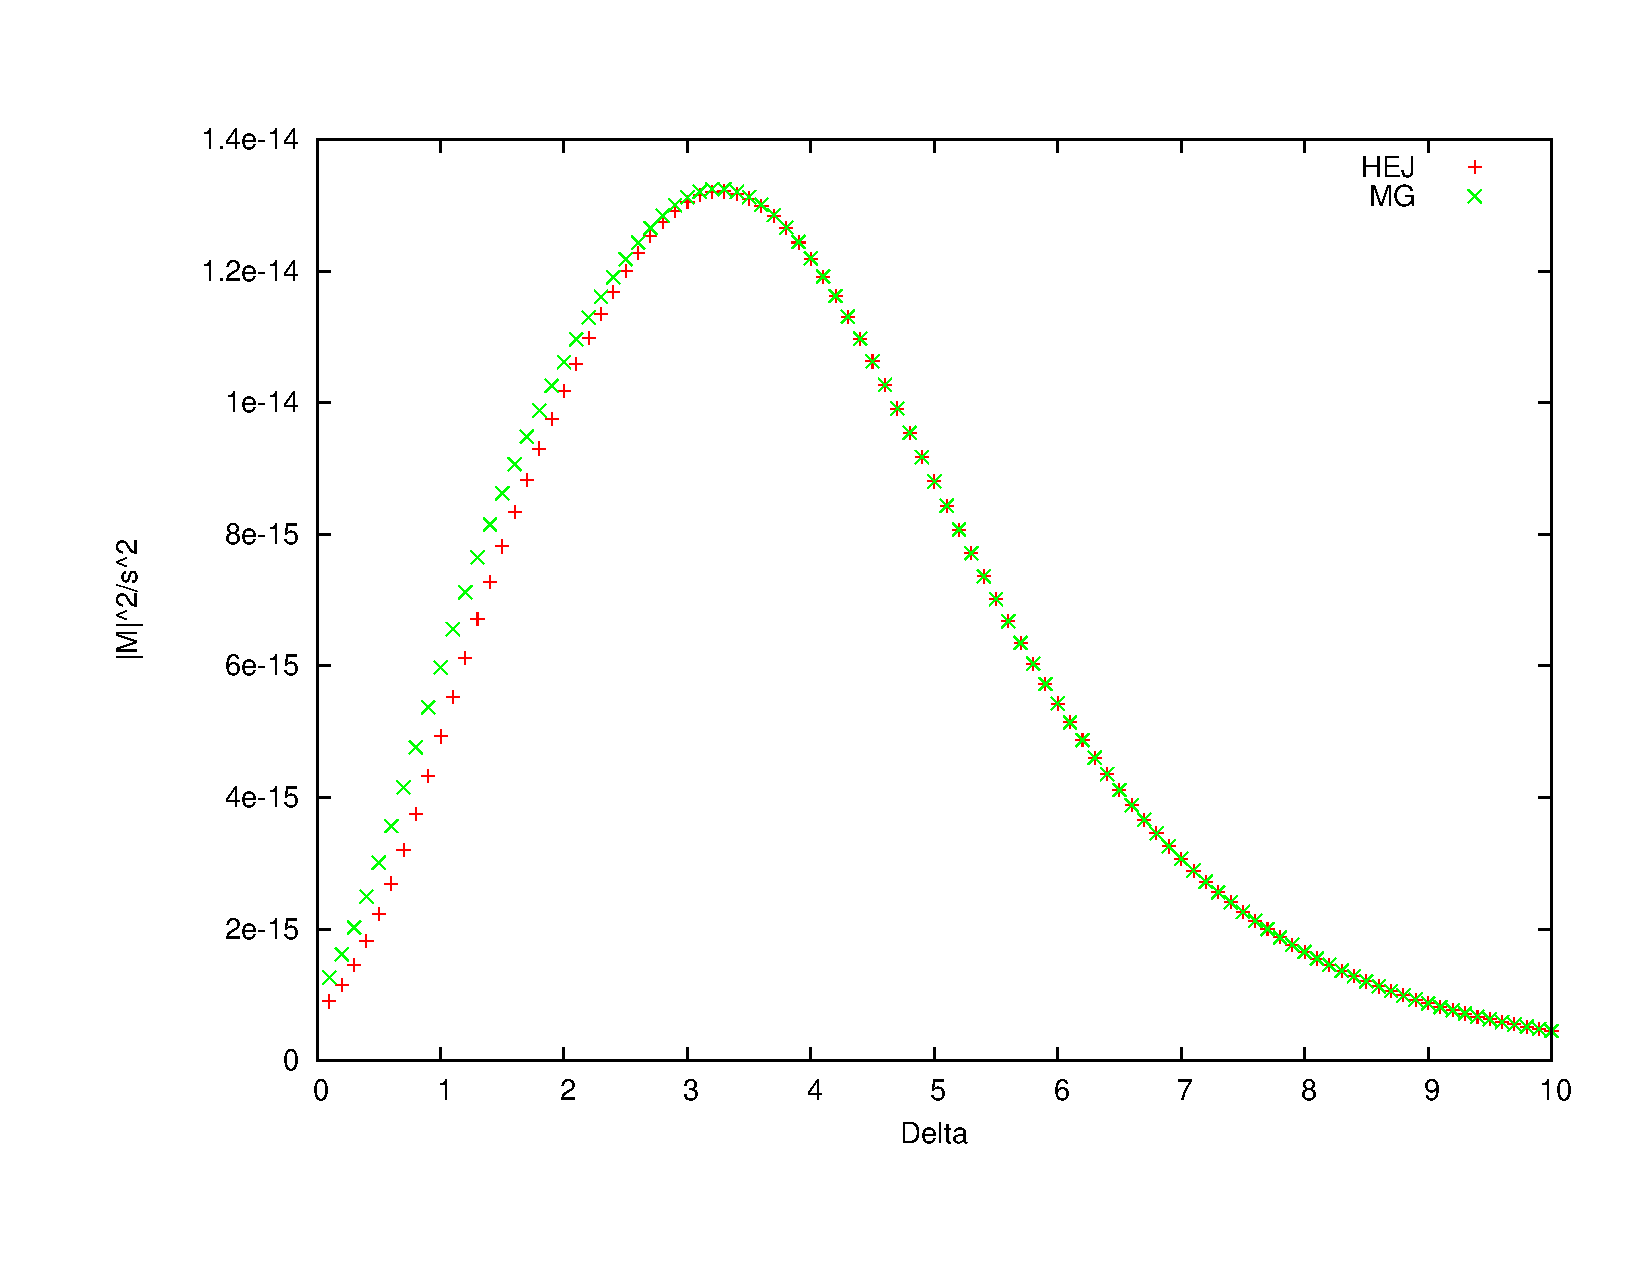
\includegraphics[scale=0.45]{Images/qQ_qqqxQ.pdf}
\caption{Effective vertex approach to the $qq' \to qQ\bar{Q}q'$ amplitude (red) compared to the full LO (green).}
\label{fig:qq_qqqq}
\end{figure}

\begin{figure}[H]
\centering
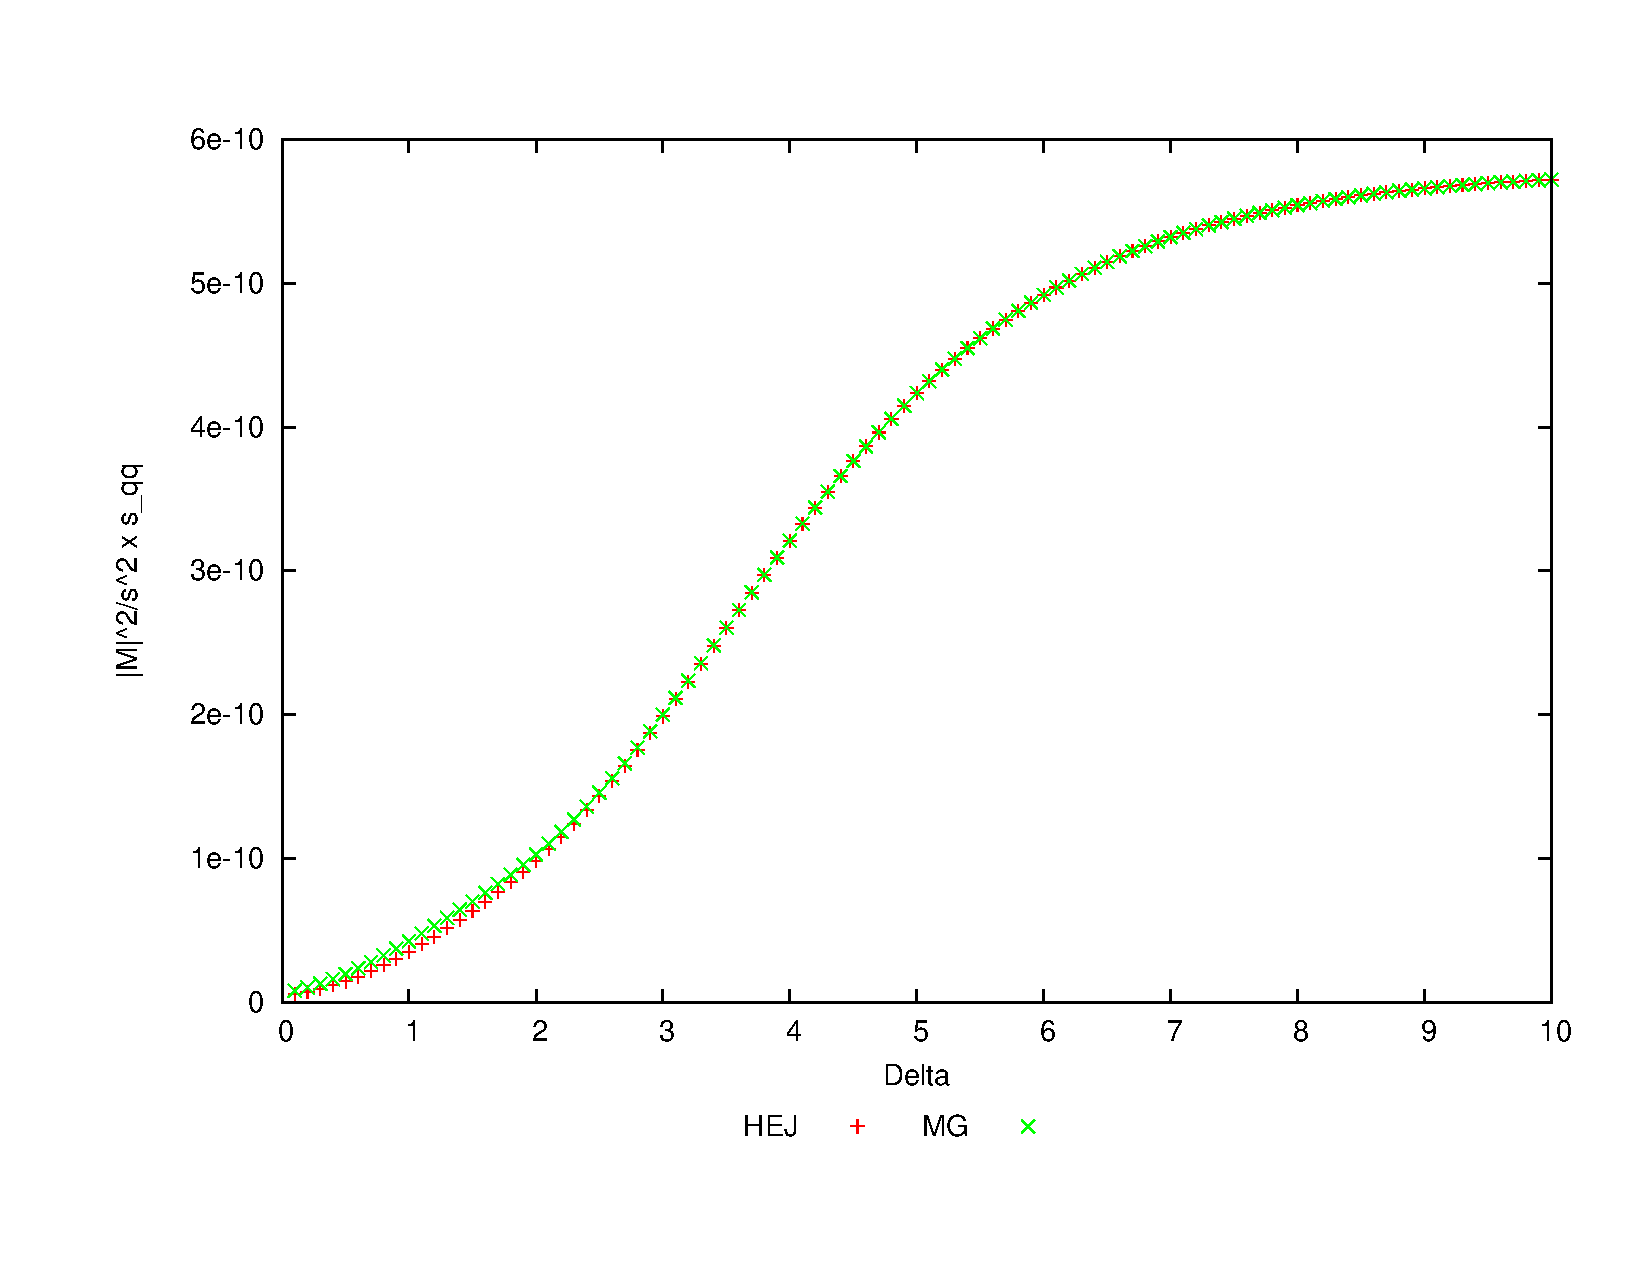
\includegraphics[scale=0.45]{Images/qQ_qqqxQ_sqqx.pdf}
\caption{Effective vertex approach to the $qq' \to qQ\bar{Q}q'$ amplitude (red) compared to the full LO (green) multiplied by the invariant mass of the quark/anti-quark pair.}
\label{fig:qq_qqqq_sqq}
\end{figure}

To extend our result to take into account gluons in the initial state, we once more multiply by colour factors:
\begin{equation}
\begin{split}
|M_{qg \to qQ\bar{Q}g}|^2 &\sim \frac{\tilde{C}_A}{C_F} |M_{qq' \to qQ\bar{Q}q'}|^2, \\
|M_{gg \to gQ\bar{Q}g}|^2 &\sim \left(\frac{\tilde{C}_A}{C_F}\right)^2 |M_{qq' \to qQ\bar{Q}q'}|^2.
\end{split}
\end{equation}
The comparison to the full leading order result for these amplitudes (multiplied by $s_{Q\bar{Q}}$) is shown in figures \ref{fig:qg_qqqg} and \ref{fig:gg_gqqg} respectively. 

\begin{figure}[H]
\centering
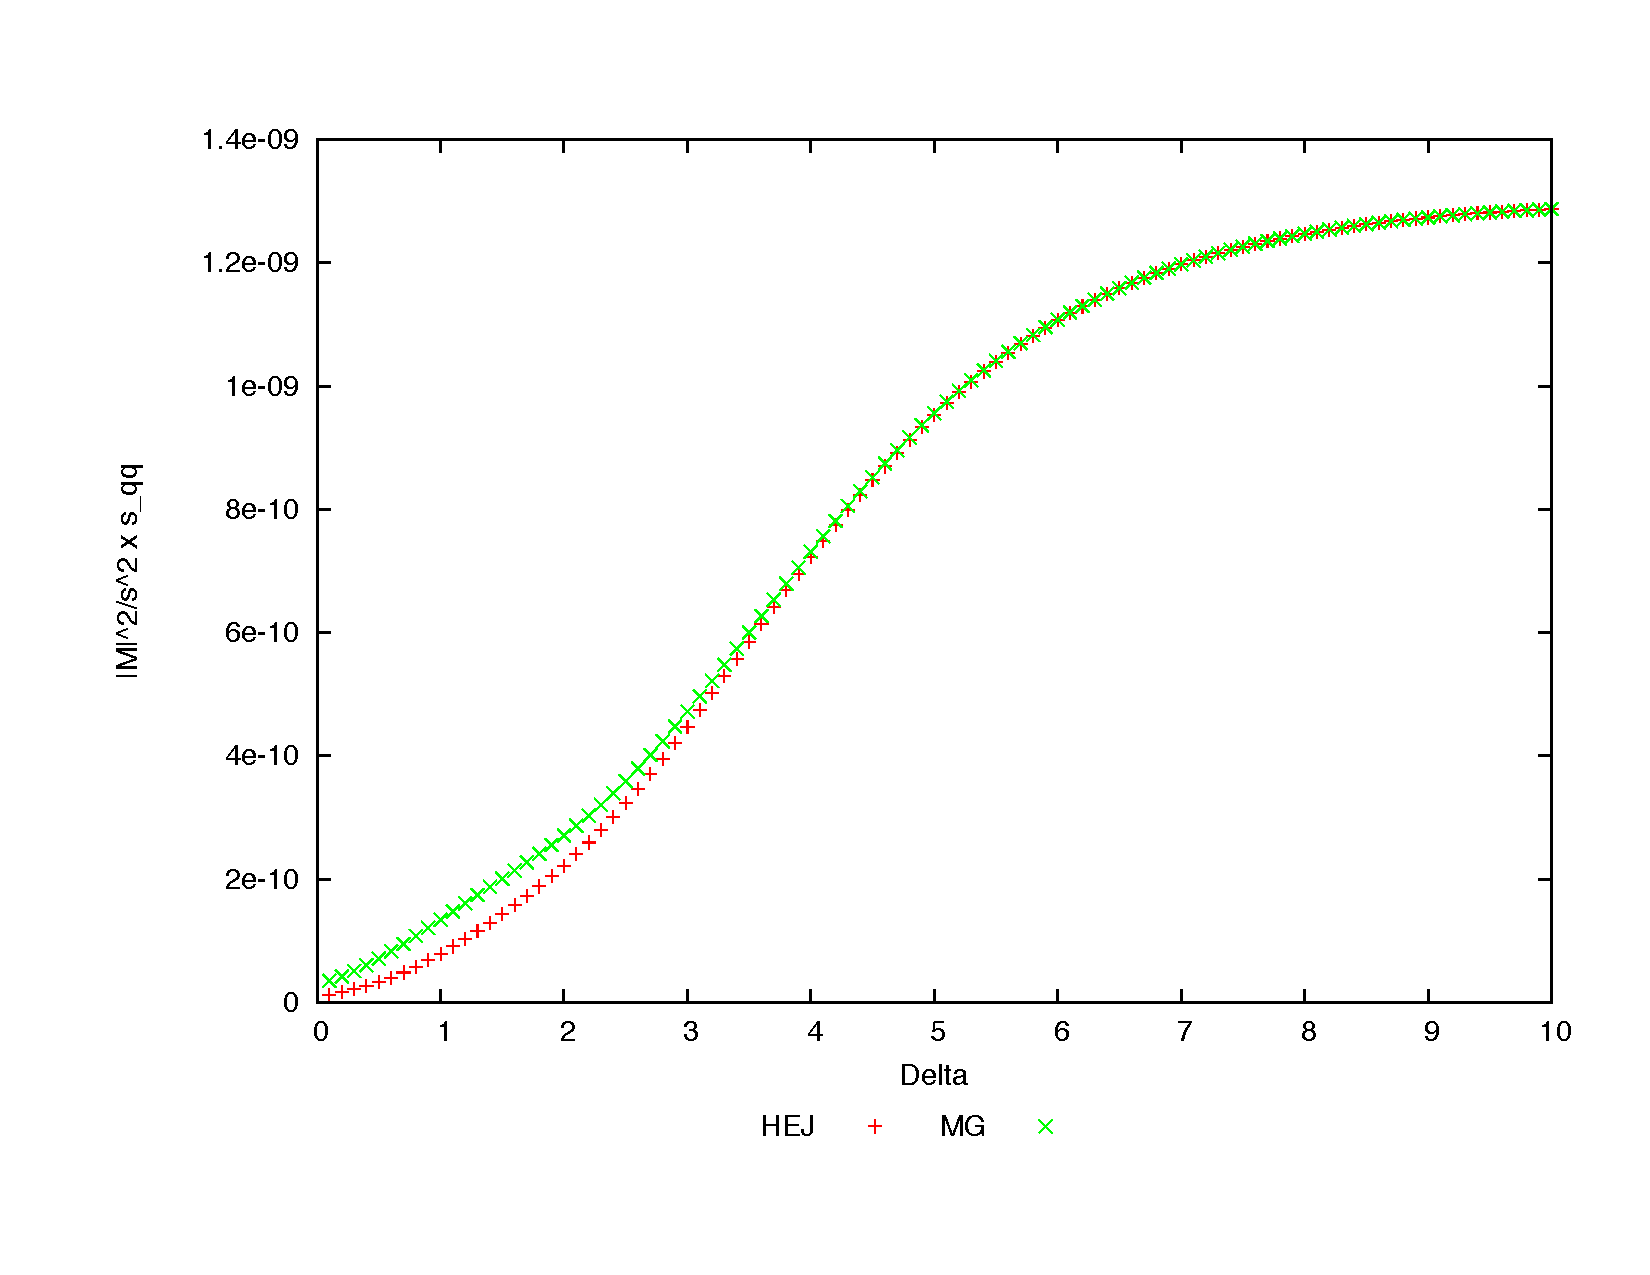
\includegraphics[scale=0.47]{Images/qg_qqqxg_sqq_simplecf.pdf}
\caption{Effective vertex approach to the $qg \to qQ\bar{Q}g$ amplitude (red) compared to the full LO (green) multiplied by the invariant mass of the quark/anti-quark pair.}
\label{fig:qg_qqqg}
\end{figure}

\begin{figure}[H]
\centering
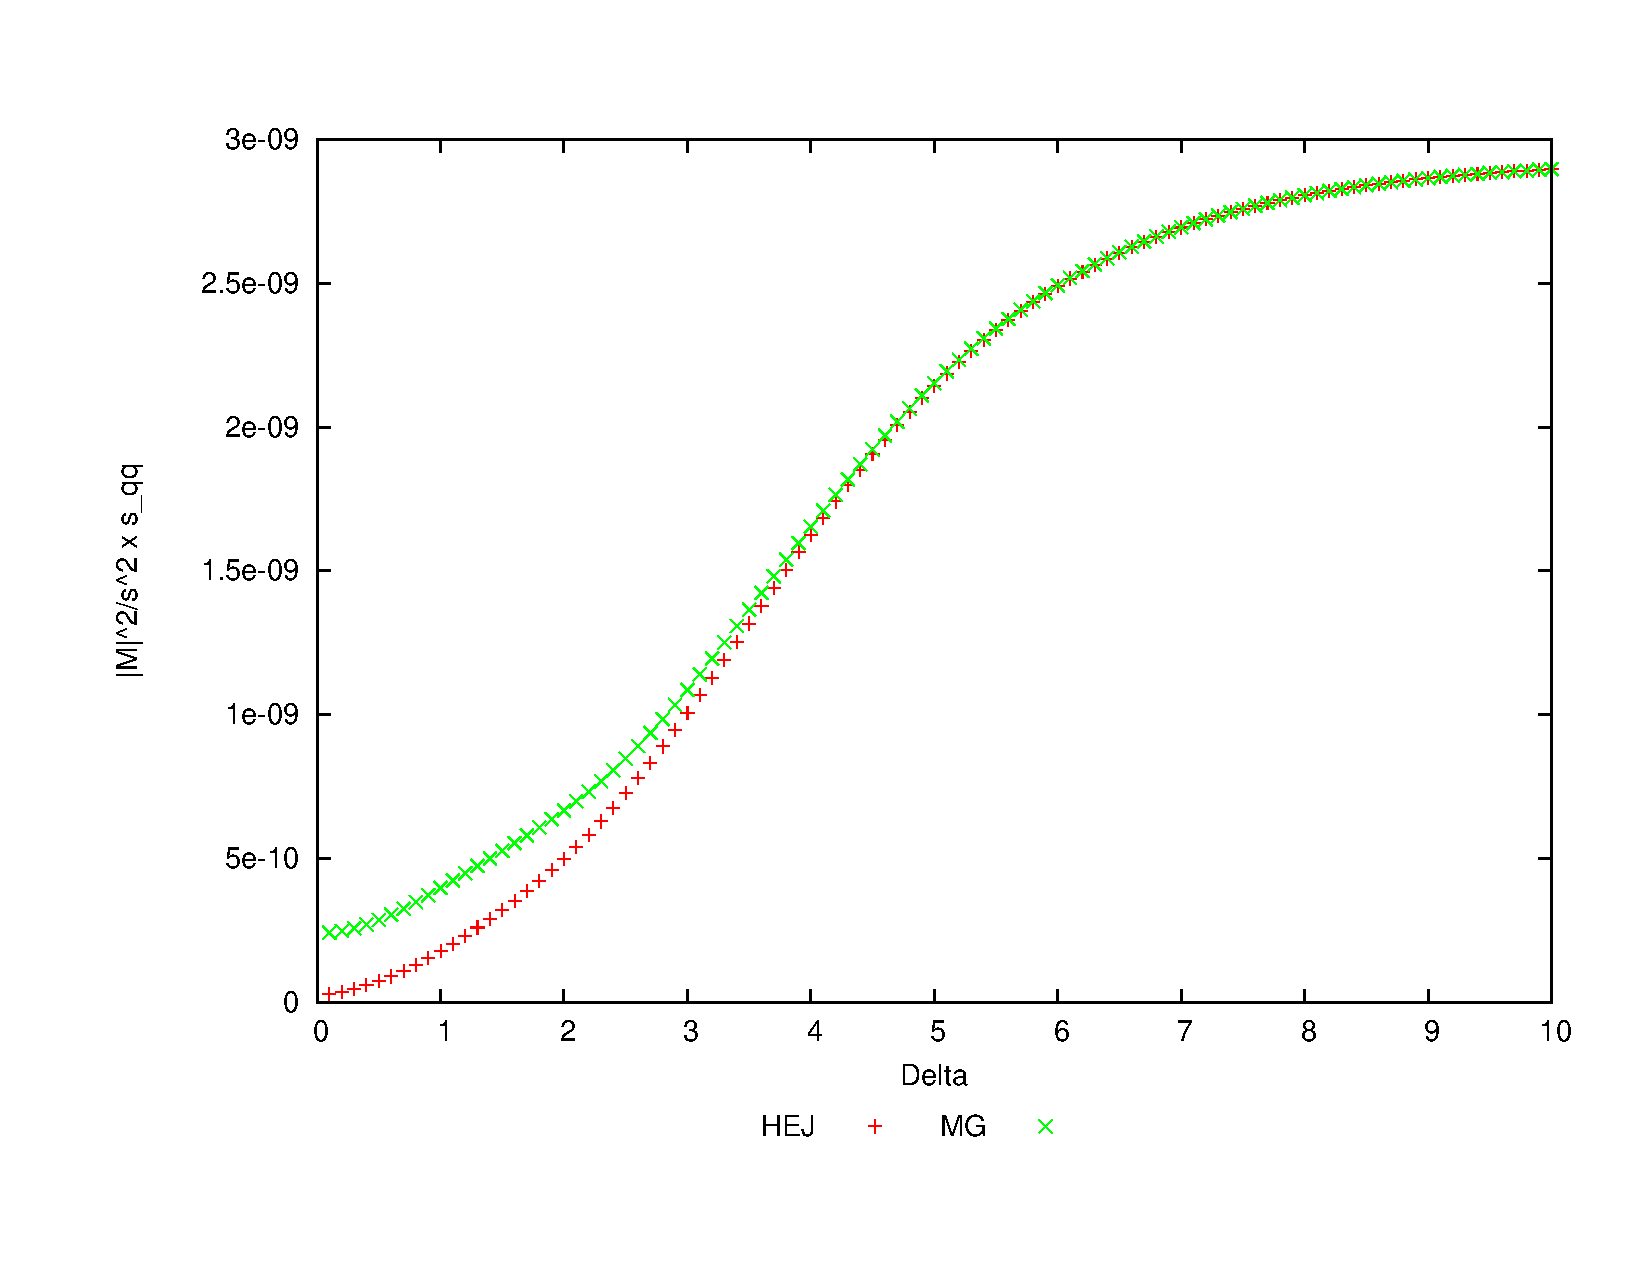
\includegraphics[scale=0.47]{Images/gg_gqqxg_sqq_simplecf.pdf}
\caption{Effective vertex approach to the $gg \to gQ\bar{Q}g$ amplitude (red) compared to the full LO (green) multiplied by the invariant mass of the quark/anti-quark pair.}
\label{fig:gg_gqqg}
\end{figure}

In this case, the addition of extra gluon emissions is slightly more complicated than in the previous case. Any extra emission can take place either before or after the effective central vertex in the rapidity chain, as shown in figure \ref{fig:5jet_choice}. This distinction needs to be kept track of and so our extension is
\begin{equation}
\begin{split}
|M_{qq' \to q...Q\bar{Q}...q'}|^2 &= |M_{qq' \to qQ\bar{Q}q'}|^2 \times \prod_{i=1}^{n_a} C_A \left(\frac{-V(q_i,q_{i+1}) \cdot V(q_i,q_{i+1})}{q_{i+1}^2} \right) \\
&\times \prod_{j=n_a+2}^{n-2} C_A \left(\frac{-V(q_j,q_{j+1}) \cdot V(q_j,q_{j+1})}{q_j^2} \right),
\end{split}
\end{equation}
\begin{figure}[t]
\centering
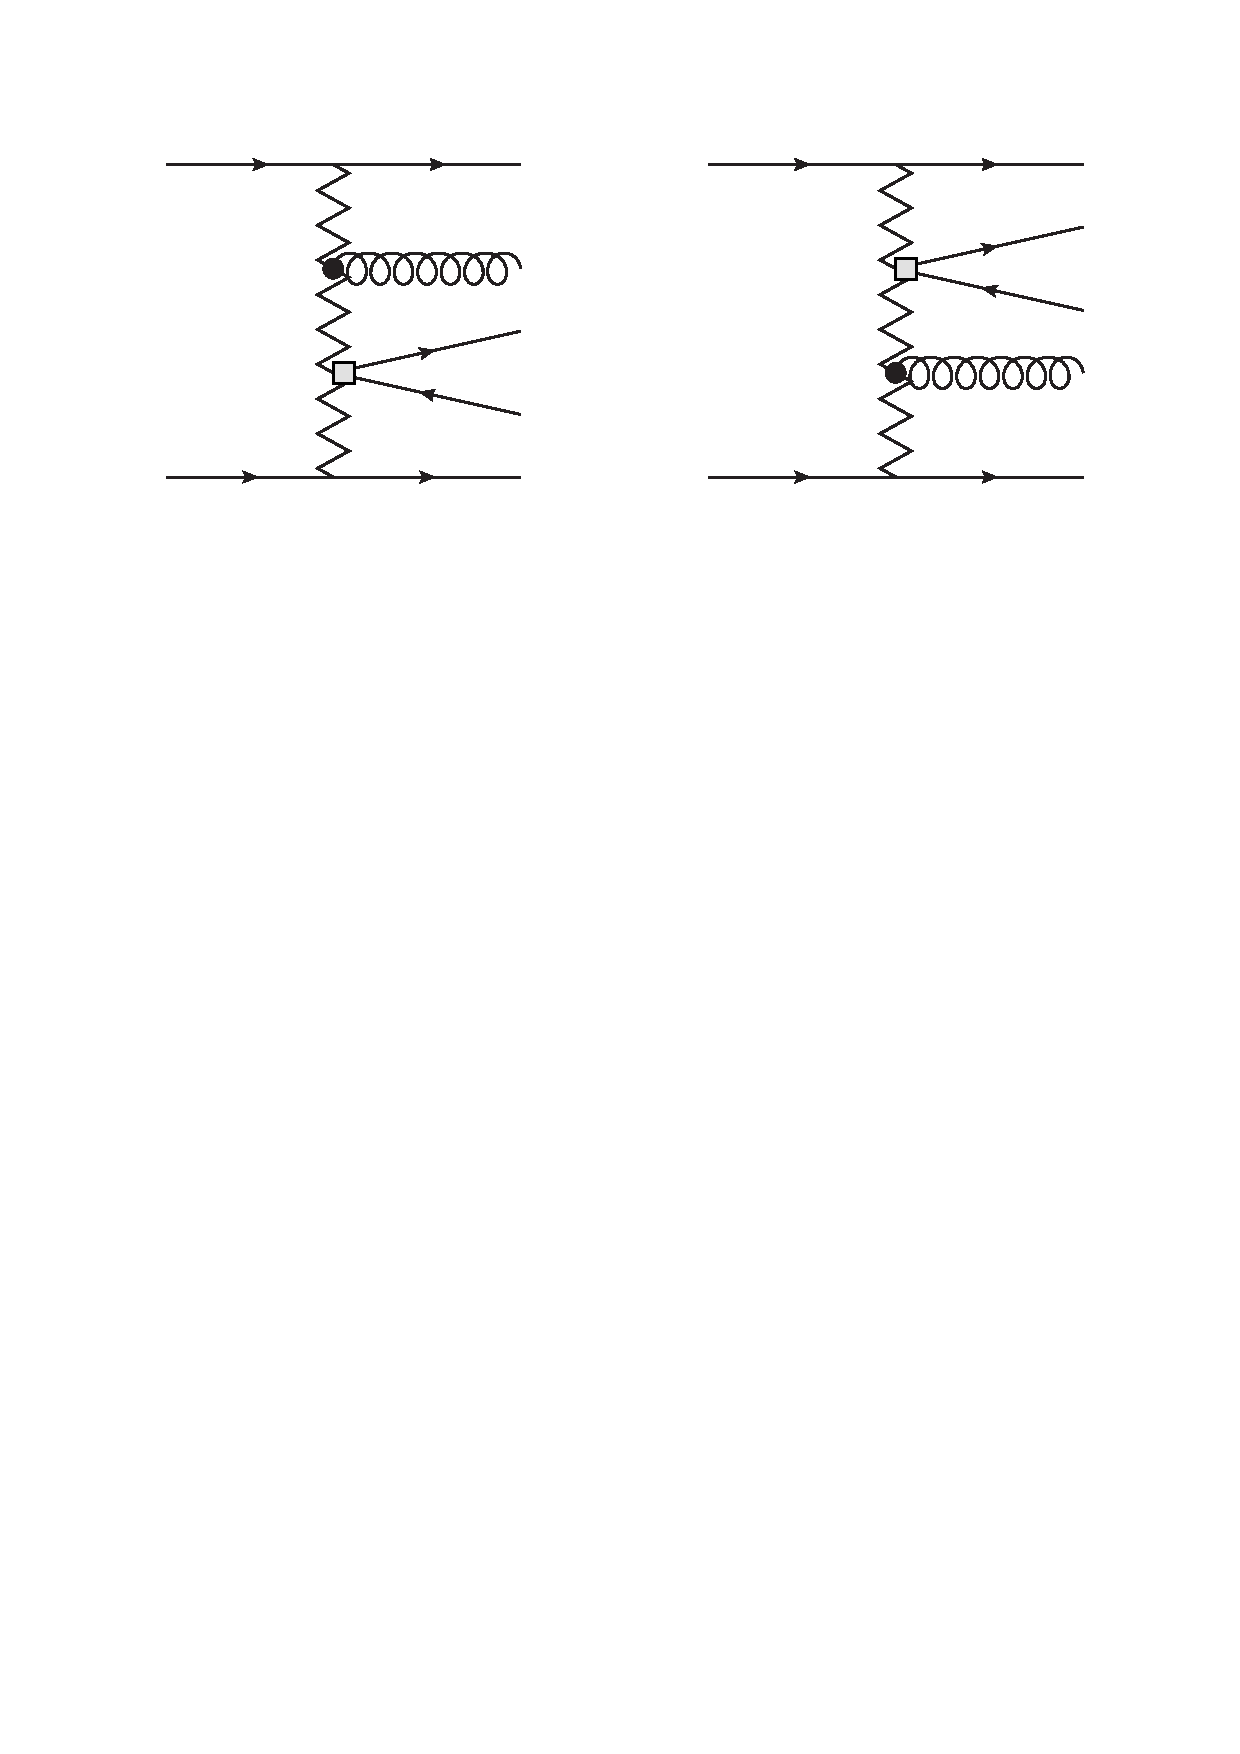
\includegraphics[scale=0.75]{Images/5jet_choice.pdf}
\caption{Extra gluon emissions can be either before (left) or after (right) the central $Q\bar{Q}$ vertex in rapidity.}
\label{fig:5jet_choice}
\end{figure}
where $n_a$ is the number of gluons more forward in rapidity than the quark/anti-quark pair. We take the simplest case of adding just one extra emission and investigate the amplitude for both options. We employ the following set of five jet momenta:
\begin{equation}
\begin{split}
p_1 & = (40 \cosh(\Delta), 0, 40, 40 \sinh(\Delta)), \\
p_2 & = (40 \cosh(\Delta/2), -40, 0, 40 \sinh(\Delta/2)), \\
p_3 & = (80 \sqrt{2}, 80, -80, 0), \\
p_4 & = (40 \cosh(-\Delta/2), -40, 0, 40 \sinh(-\Delta/2)), \\
p_5 & = (40 \cosh(-\Delta), 0, 40, 40 \sinh(-\Delta)). 
\end{split}
\end{equation}
In figure \ref{fig:central_gfor} we plot the result for when the gluon is more forward in rapidity than the $Q\bar{Q}$ pair and in figure \ref{fig:central_gback} we have the result for when it is emitted more backward in rapidity. Both of these figures show reasonable agreement with the full result and importantly, agree precisely in the high energy limit. 

\begin{figure}[H]
\centering
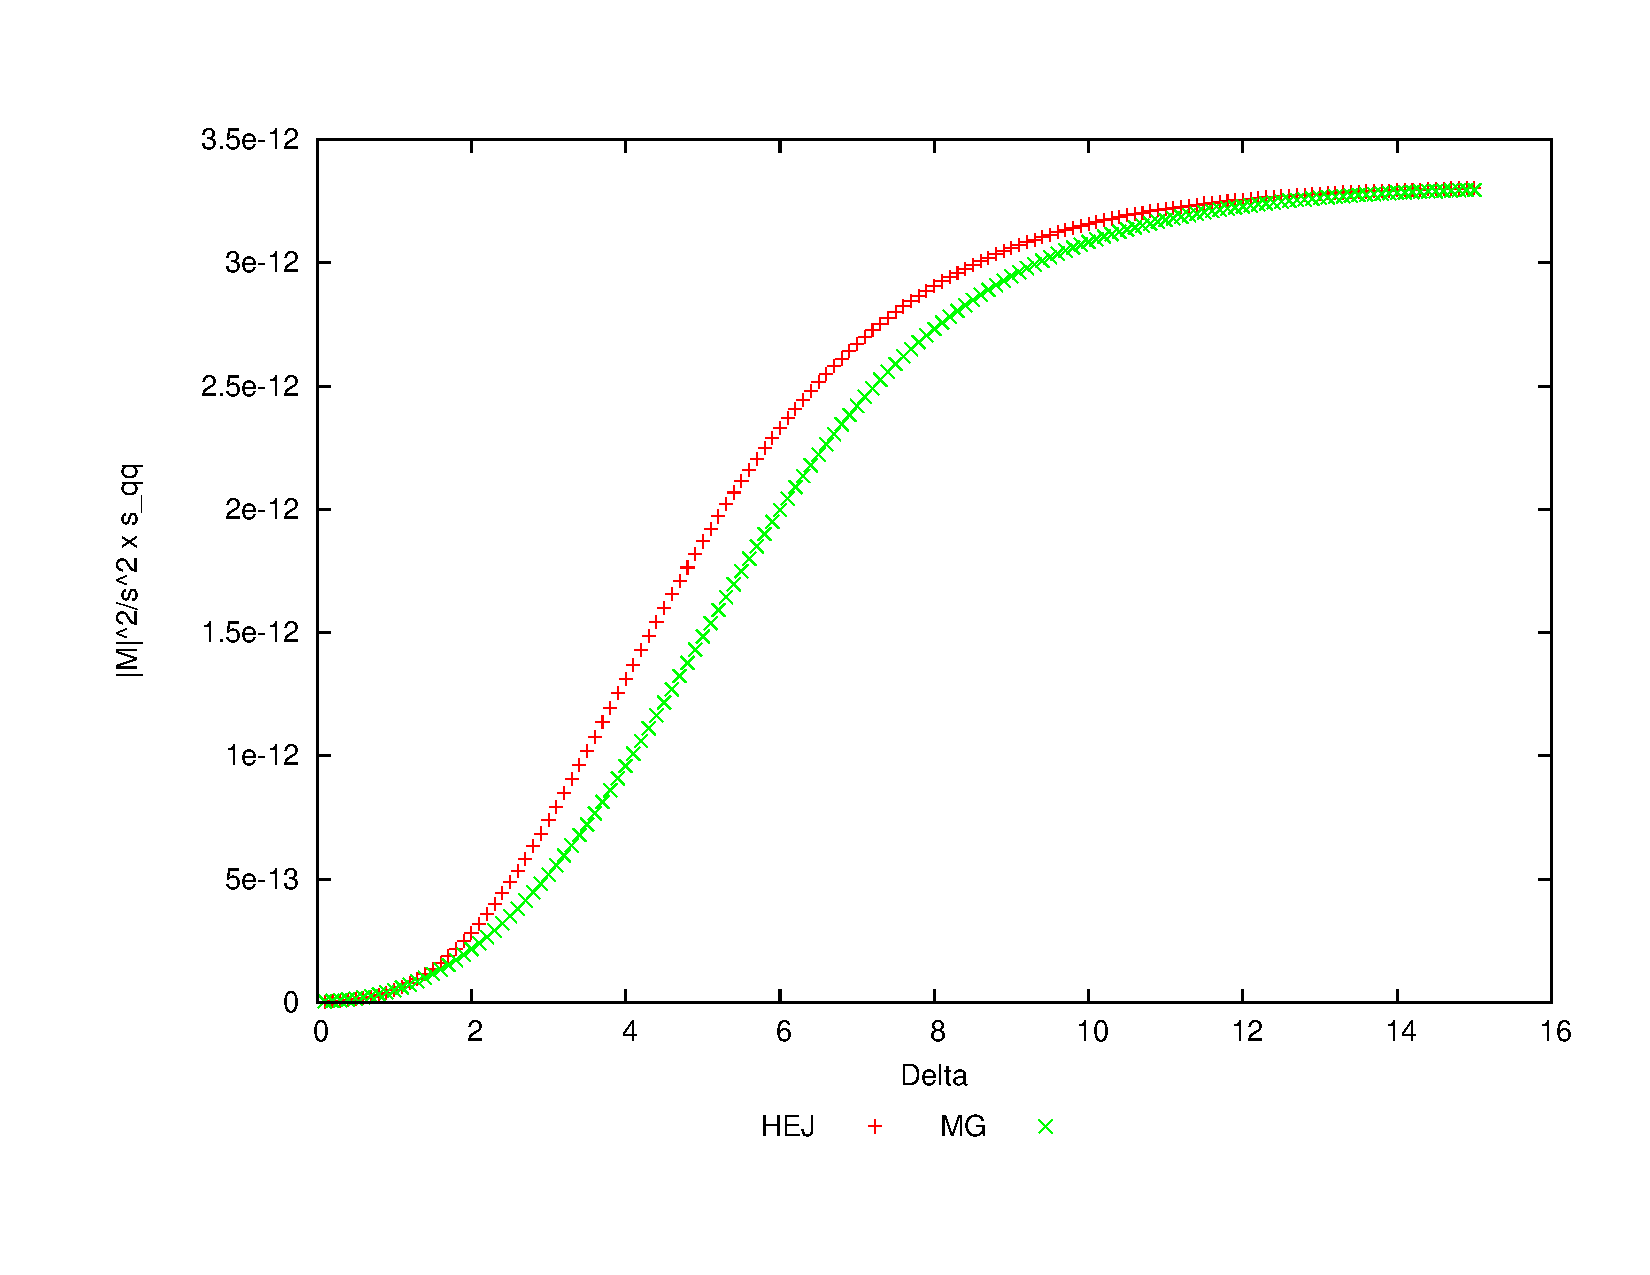
\includegraphics[scale=0.44]{Images/qQ_qgqqxQ_sqq.pdf}
\caption{Effective vertex approach to the $qq' \to qgQ\bar{Q}q'$ amplitude (red) compared to the full LO (green) multiplied by the invariant mass of the quark/anti-quark pair.}
\label{fig:central_gfor}
\end{figure}

\begin{figure}[H]
\centering
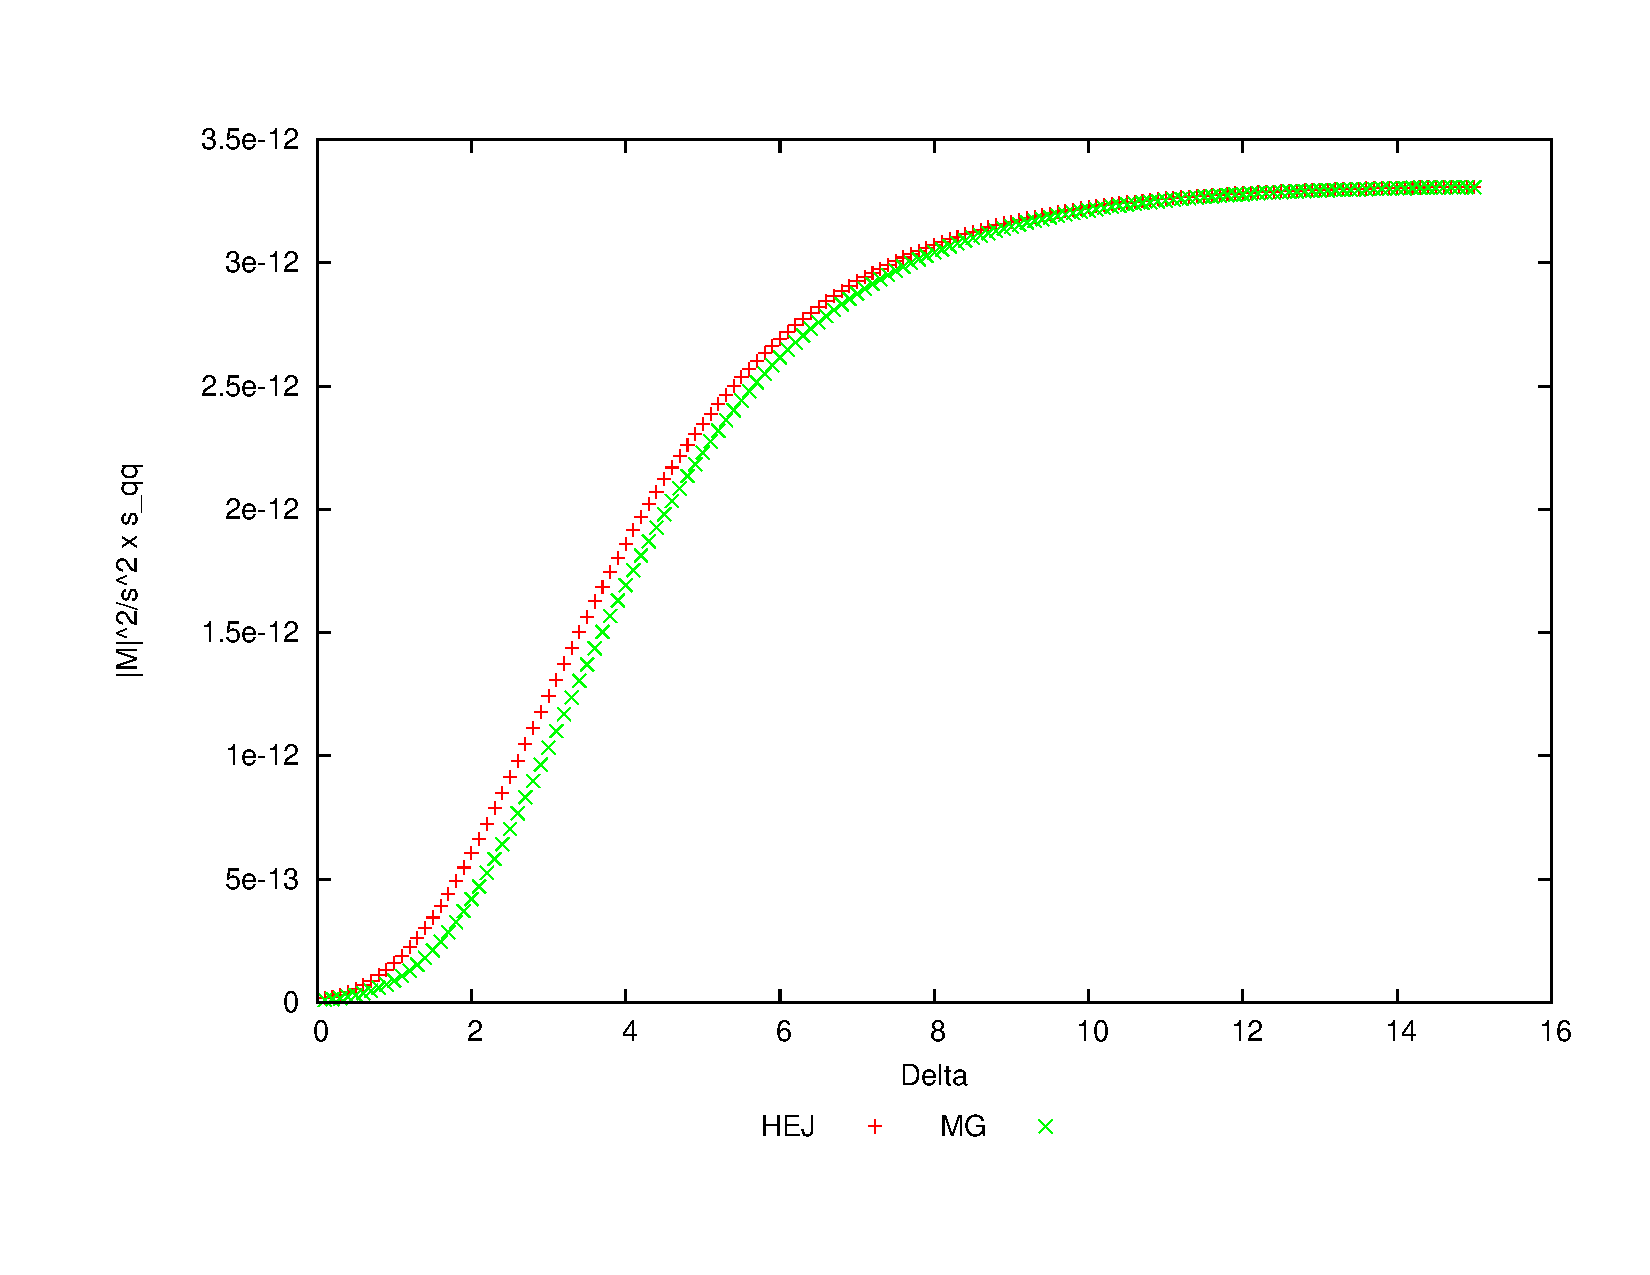
\includegraphics[scale=0.44]{Images/qQ_qqqxgQ_sqq.pdf}
\caption{Effective vertex approach to the $qq' \to qQ\bar{Q}gq'$ amplitude (red) compared to the full LO (green) multiplied by the invariant mass of the quark/anti-quark pair.}
\label{fig:central_gback}
\end{figure}

\section{Computational Aspects}
%\todo{removing from nonFKL, generating all possible processes, making sure matching is done consistently} 
The explorer plots of the last two sections all serve to convince that the derived amplitudes behave as expected. The next step is to include them in the full HEJ program correctly. This is a very significant change to the codebase that requires the modification of many files and so a `branch' of the codebase was created so that all work can be done independently of other projects going on in the collaboration. Once everything is completed and checked, the branch can be merged back into the main development codebase in a way that does not disrupt any other work done there since the branch was created. The points that need to be considered when adding these amplitudes in are as follows:

\begin{enumerate}
\item{Correctly removing calls to fixed order non-FKL processes if they are now to be included in the resummation. For example, the code already contains a call to the $qg \to qQ\bar{Q}$ amplitude at leading order for matching purposes as discussed in section 2.5. We therefore need to remove calls to these particular subprocesses in that section of the code but only if the user specifies that they wish to include these processes in the resummation (although it will become default for HEJ to include them). }
\item{Ensuring that all possible processes are generated. Since the HEJ program is a Monte Carlo program, we must ensure that all of these extra NLL processes are `picked'. Since we require a leading order matching, one consideration is that a new process should not be picked if the event will not cluster into at least three jets. Also, given a set number of final state partons and a central $Q\bar{Q}$ emission, we must make sure that all positions of that emission along the rapidity chain are considered. Another point is that the rapidity ordering of the $Q\bar{Q}$ pair can be either way around (quark/anti-quark or anti-quark/quark) and we must include both orderings. Failure to do any of this correctly will mean that the program will be artificially removing physics that we know should be included.}
\item{Checking that the leading order matching at the jet level for the NLL processes is done consistently. For example, imagine we generate a central $Q\bar{Q}$ emission at the parton level and choose partons $p_i$ and $p_j$ for the pair, where $p_i$ is more forward than and next to $p_j$ in rapidity. In order to properly implement the matching, we require that these cluster into two different jets, $p_i \to j_i$ and $p_j \to j_j$, where $j_i$ is more forward than and next to $j_j$ in rapidity. Because of how the clustering works, it is not at all guaranteed that the jets will preserve this rapidity ordering; moreover, these jets might not even still be next to each other in rapidity in the chain. All these considerations must be carefully checked by looking at the jet constituents.}
\end{enumerate} 
It is absolutely crucial that all of these points are properly addressed and checked and such a task is necessarily time-consuming. After validating these steps by comparisons to old code with certain constraints, we can be confident that everything works as it should. In the following two sections, we move on to discuss how the inclusion of these NLL processes affects HEJ in practice. 

\section{Full Phase Space Analysis}

One important advantage of now being able to resum these partonic subprocesses and unordered events is that it means we have a reduced reliance on fixed-order matching codes. In chapter 2, we showed how `non-FKL' contributions are sub-leading in the High Energy Limit. While this is true, there are regions that (for example) the LHC can probe which are clearly not well-described by the High Energy Limit. For instance, we could imagine a region where one parton's $p_T$ is very large, creating a significant $p_T$ hierarchy that the High Energy Limit assumes not to be there. In order for HEJ to be competitive as a prediction over the entirety of the explored phase space, we need to include some description of these types of process, which we do via the inclusion of fixed-order (currently LO) matrix elements. We have shown here that some of these non-FKL processes can themselves be resummed and therefore can be removed from the fixed-order samples. In this section, we investigate the impact of this when we integrate over all of the relevant phase space. In the following figures, we show the total cross-section for inclusive 3 jets, broken down into the contribution coming from the resummation and the fixed order. It is desirable in these plots if the red line (the resummed contribution) is as close to the black line (the total contribution) as possible. For completeness, the relevant cuts applied were $p_{T,min} = 30$ GeV, $y_{max} = 4.4$, and $\sqrt{s} = 13$ TeV. 

In figure \ref{fig:fklmigration}, we show a `before and after' comparison of the $m_{fb}$ distribution. It is clear that that the inclusion of these extra processes dramatically reduces the contribution of fixed-order matrix elements across the range, but especially in the low bins. The contribution of the non-FKL processes to the total cross-section in these bins is approximately 43\% in the top plot, which drops to around 15\% in the bottom. In the high bins, the contribution drops from around 15\% to almost zero. 

In figure \ref{fig:fklmigration2}, we show the events binned instead in the $p_T$ of the hardest jet. In it, we see that a significant proportion of the fixed order matrix elements that were very significant in the high $p_T$ region (contributing close to 60\% of the cross-section there) are now included in the resummation. The net effect is to reduce the non-FKL contribution to the total cross-section down to 20\%. 

Finally, in figure \ref{fig:fklmigration3} we show the analysis broken up in bins of the rapidity difference between the most forward and backward jets. There, we once more see a substantial improvement across the board, with the largest non-FKL percentage contribution of 30\% being reduced to 12\%. In the higher bins, we once more see evidence that the non-FKL contributions are tending to zero. 

\begin{figure}[H] 
\centering
\subfloat{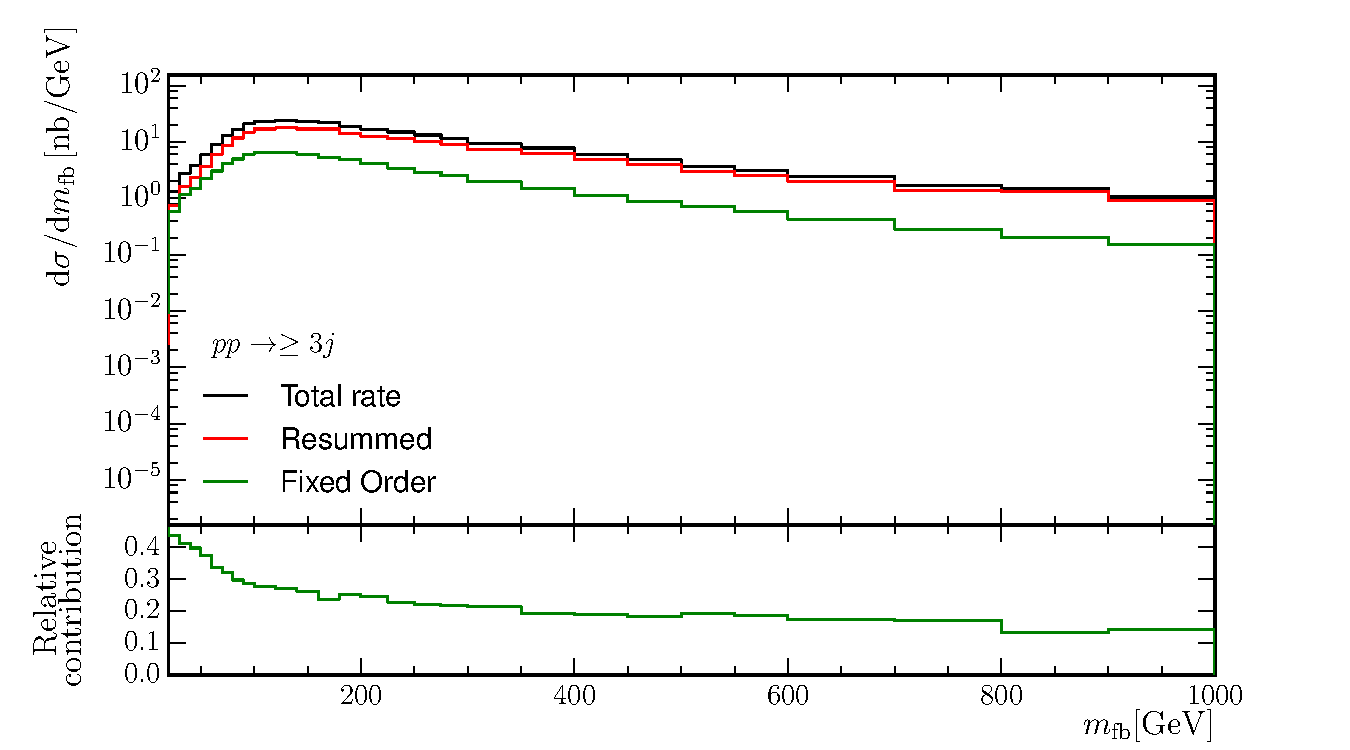
\includegraphics[scale=0.7]{Images/mfb_3jinc_bare_breakdown.pdf}} \\
\subfloat{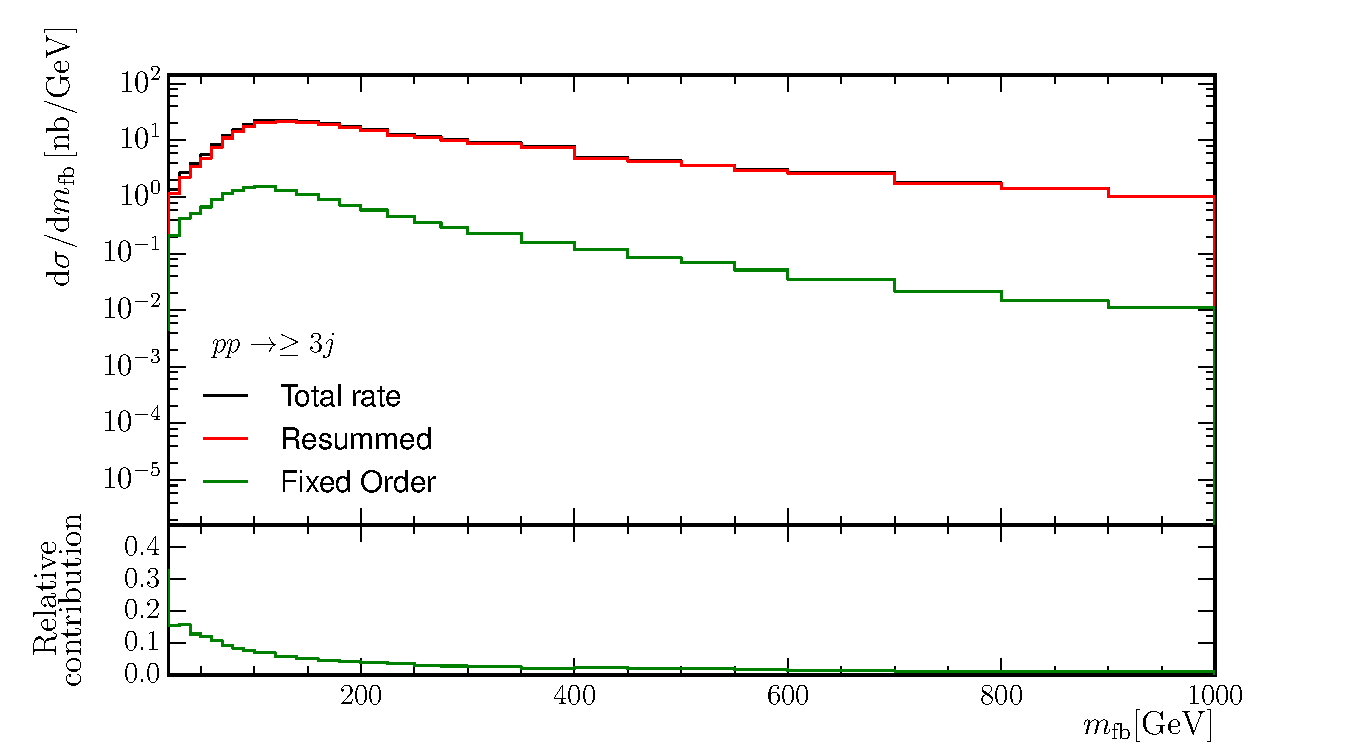
\includegraphics[scale=0.7]{Images/mfb_3jinc_resummed_breakdown.pdf}}
\caption{A breakdown of contributing parts to the jet cross section before (top) and after (bottom) implementing the effective vertex description of the new partonic subprocesses and the unordered events, in bins of the invariant mass between the most forward and backward jets.}
\label{fig:fklmigration}
\end{figure}

\begin{figure}[H] 
\centering
\subfloat{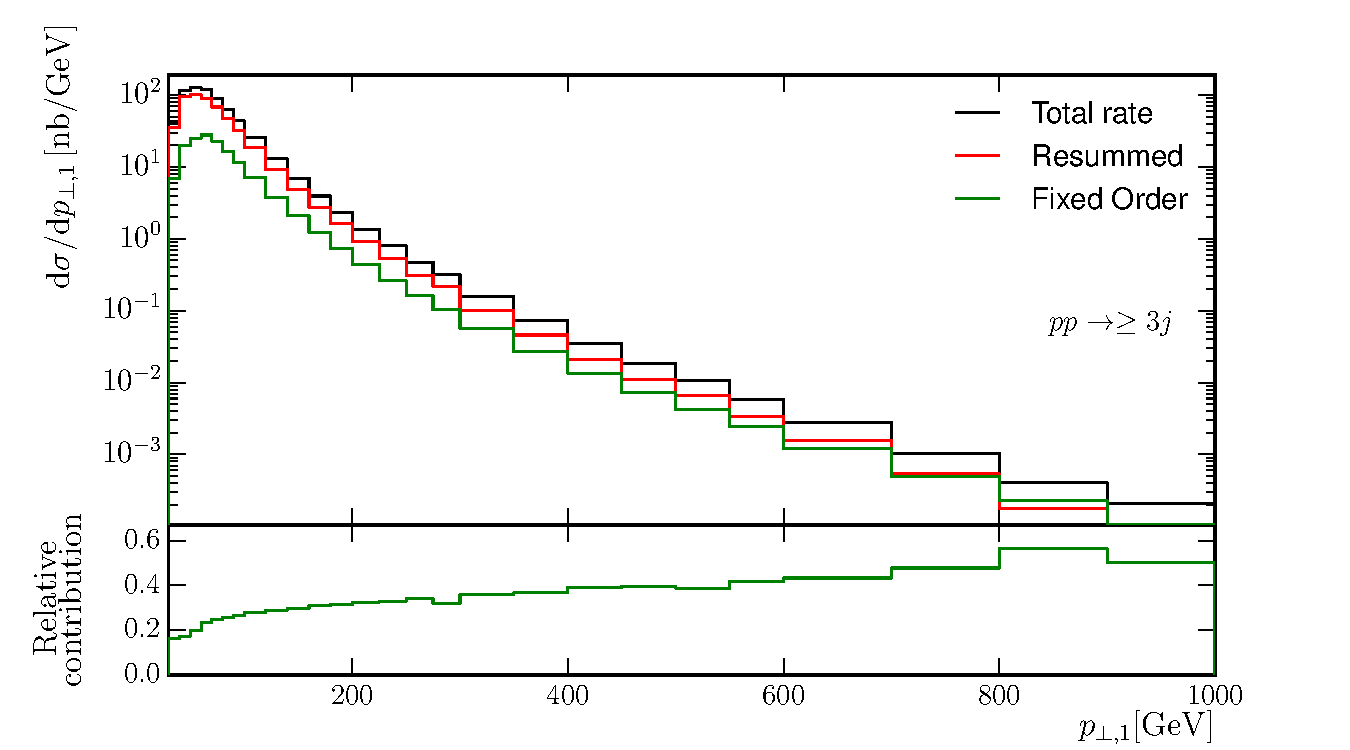
\includegraphics[scale=0.7]{Images/pt1_3jinc_bare_breakdown.pdf}} \\
\subfloat{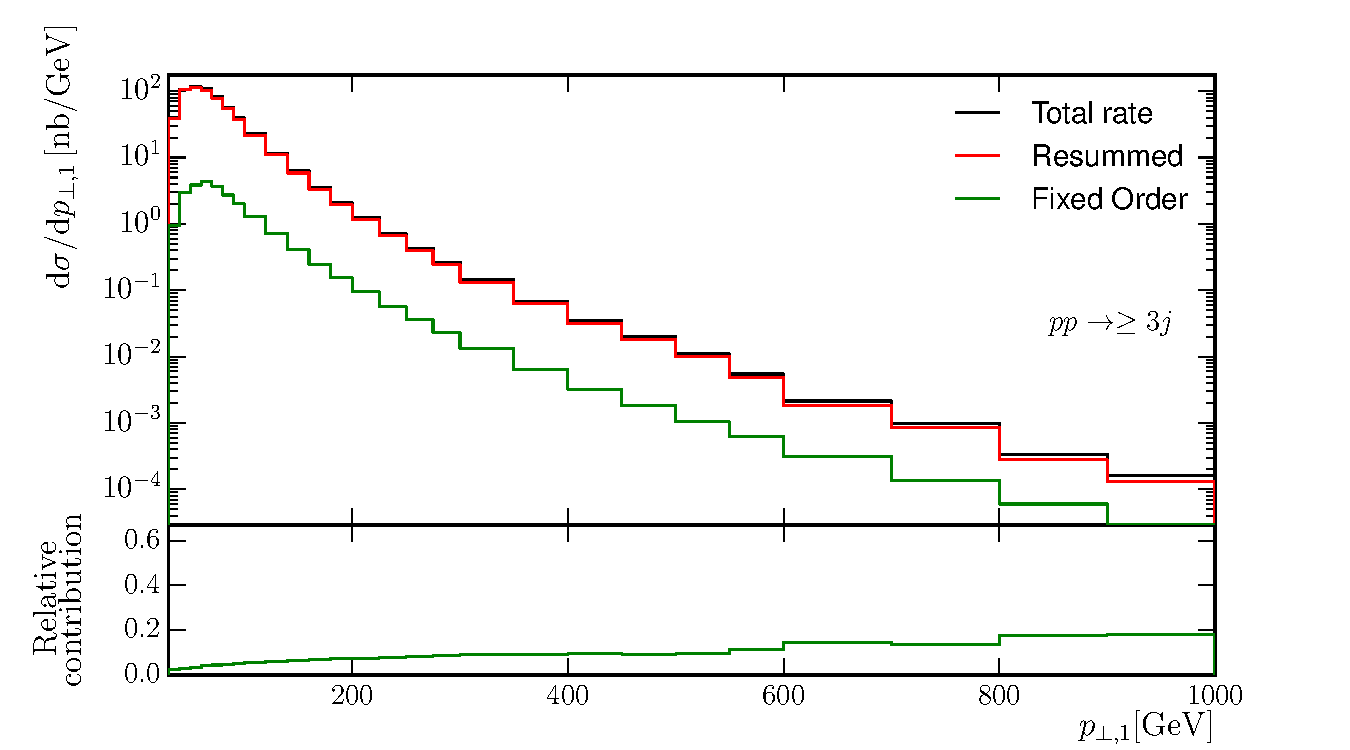
\includegraphics[scale=0.7]{Images/pt1_3jinc_resummed_breakdown.pdf}}
\caption{A breakdown of contributing parts to the jet cross section before (top) and after (bottom) implementing the effective vertex description of the new partonic subprocesses and the unordered events, in bins of the $p_T$ of the hardest jet.}
\label{fig:fklmigration2}
\end{figure}

\begin{figure}[H] 
\centering
\subfloat{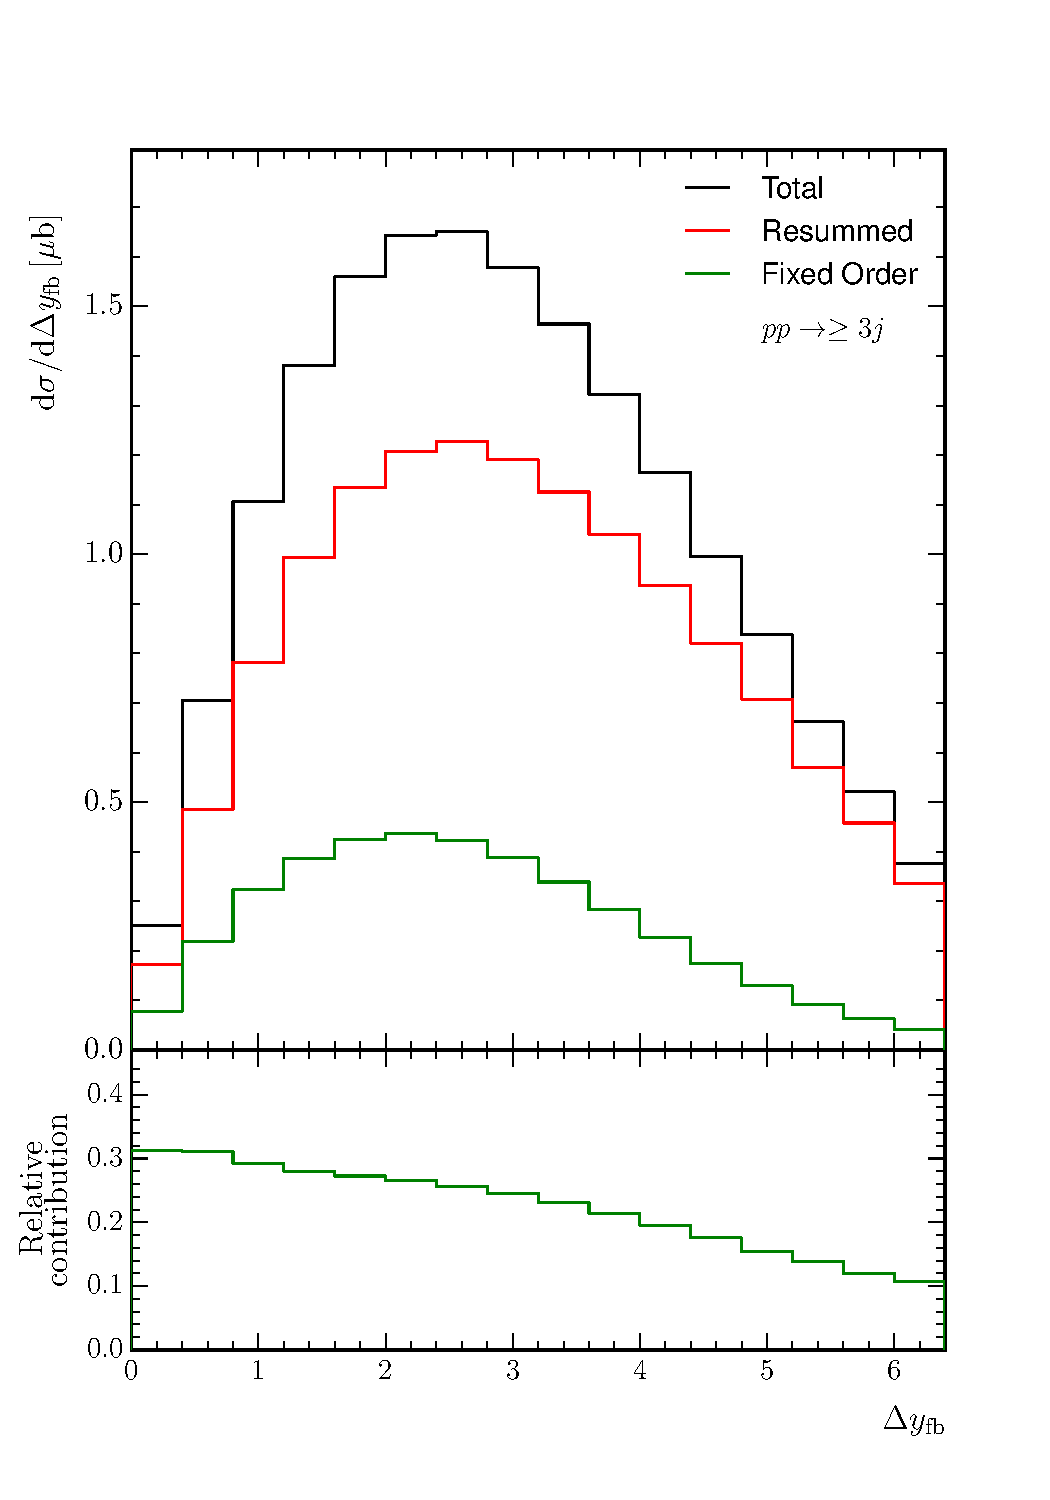
\includegraphics[scale=0.45]{Images/dyfb_3jinc_bare_breakdown.pdf}} 
\subfloat{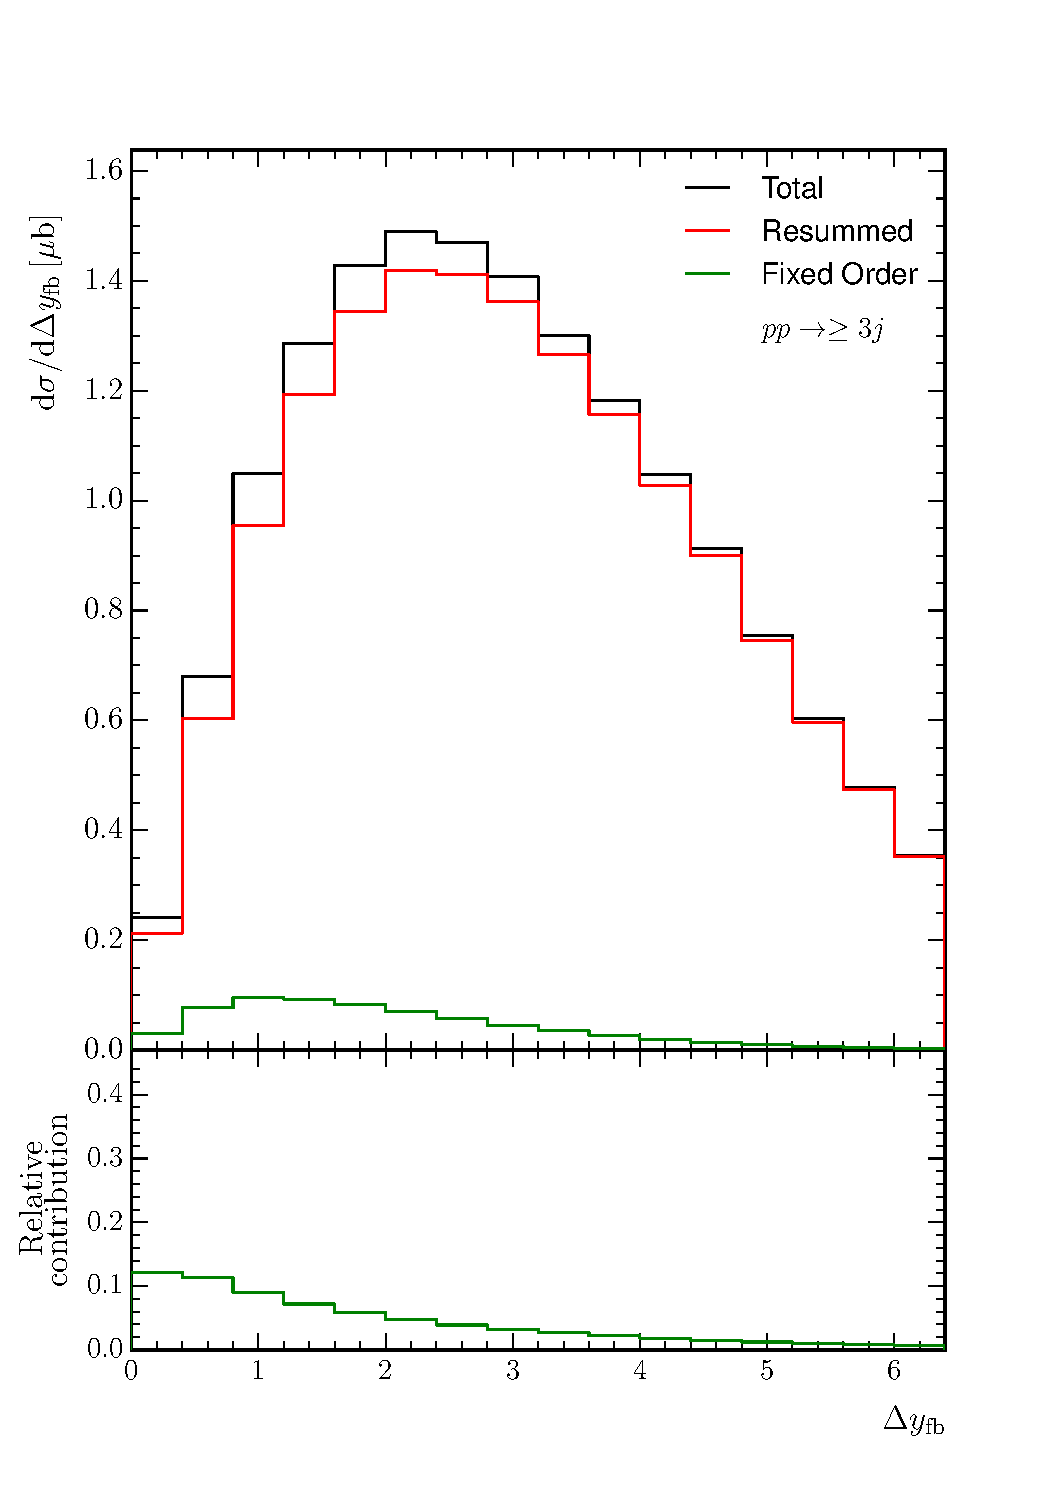
\includegraphics[scale=0.45]{Images/dyfb_3jinc_resummed_breakdown.pdf}}
\caption{A breakdown of contributing parts to the jet cross section before (left) and after (right) implementing the effective vertex description of the new partonic subprocesses and the unordered events, in bins of the rapidity difference between the most forward and backward jets.}
\label{fig:fklmigration3}
\end{figure}

\section{Comparisons to Data}
%\todo{Distributions, revisits to previous analyses with these effects added in, etc} 
%\todo{Label this diagram better. Add new ones from NLL paper?}
To conclude the chapter, we revisit the predictions for previous analyses HEJ was involved in and investigate how these new additions improve the predictions whilst comparing with real data; for example, in an ATLAS study of dijet production with a central jet veto \cite{Aad2011}. One interesting plot is figure 6 of that paper, which is that of the average number of jets in the `gap', defined as the rapidity region between the dijet system, which in this case is given by the two highest $p_T$ jets in a event. There are a total of four different lines, which correspond to different rapidity slices, shown in figure \ref{fig:veto} which correspond to (starting at the top) $4 \leq \Delta y < 5$, $3 \leq \Delta y < 4$, $2 \leq \Delta y < 3$ and $1 \leq \Delta y < 2$. In order to distinguish them on the graph, these lines are moved up by $3,2,1$ and $0$ units respectively. The $x$-axis is $\bar{p}_T$, which is the average of the dijet system's transverse momenta. For the high energy limit HEJ considers, we should not expect this to be a good variable to plot with respect to; the limit depends on all transverse scales being roughly the same order. At high average $p_T$, we can have a large $p_T$ hierarchy. This is indeed reflected at the right-hand side of the figure. It was noted that the analysis might have been better performed by considering only the resummed part of the HEJ calculation, since it is this part that gives rise to gap jets. We therefore include both the full and resummed-only lines in this figure. In the diagram on the top left, we see a considerable difference between these two predictions. By adding these new processes, we make these lines essentially indistinguishable and at the same time capture more bins on the left-hand side of the plots. It is advantageous for the two lines to come together like this, since it eradicates the need to arbitrarily choose just the resummed predictions over the full prediction. This is a practical consequence of our lesser reliance on fixed order matching in the formalism. Going back to the plot and we see that the addition of these NLL processes still does not tell the whole story; the correct description of the bins on the right-hand side still requires the addition of parton shower effects. Since HEJ and parton showers are designed to describe completely different regions of amplitudes, this is not surprising. 

Indeed, in a later dijet veto ATLAS analysis \cite{Aad2014}, it was observed that the predictions from the pure partonic HEJ needed to be interfaced with a parton shower in order to get the best description of the data. Although of course there are regions where a parton shower description is always going to be important, we can investigate to see if NLL effects can push the pure partonic line closer to the data by itself. For example, consider figure 3a of \cite{Aad2014}, which plots the `Gap Fraction', defined as
\begin{equation}
f(Q_0) = \frac{\sigma_{jj}(Q_0)}{\sigma_{jj}},
\end{equation}
where $\sigma_{jj}$ is the inclusive dijet cross-section and $\sigma_{jj}(Q_0)$ is the cross-section for dijet production in the absence of additional jets with transverse momentum above the threshold $Q_0$ in the rapidity interval defined by the dijet system (once more defined by the two hardest jets in the event). Such an observable will clearly be sensitive to resummation effects, since we saw earlier that the rapidity gap plays a central role in the derivation of our amplitudes. In figure \ref{fig:newveto3a} we plot a comparison of data to four different HEJ runs, which correspond to the four different combinations of including/not including the unordered/sub-leading partonic process corrections. For the same reasons as before, we plot both the resummed and full HEJ lines for comparison. The bottom-right figure shows that the inclusion of both of these effects leads to a better description of the data everywhere, but in particular we gain a few extra bins at the left side of the figure when compared to the top-left.

\begin{figure}[t]
\centering
\subfloat[No NLL corrections.]{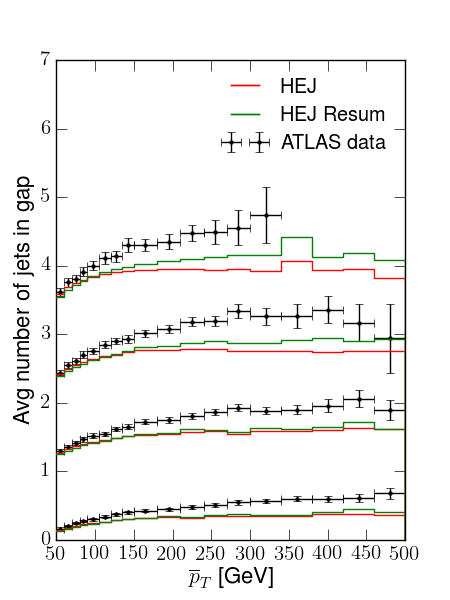
\includegraphics[scale=0.6]{Images/Veto_Plots/pf6_bare.png}}
\subfloat[Unordered corrections.]{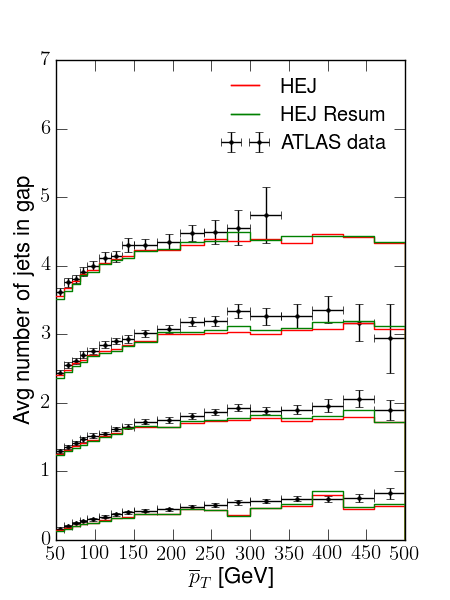
\includegraphics[scale=0.6]{Images/Veto_Plots/pf6_uno.png}} \\
\subfloat[Sub-leading partonic processes corrections.]{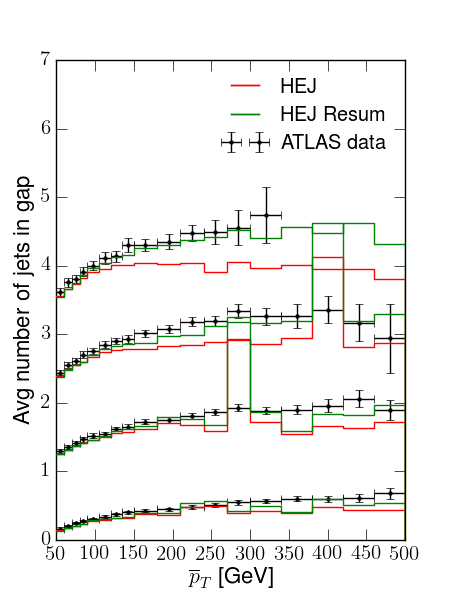
\includegraphics[scale=0.6]{Images/Veto_Plots/pf6_qqx.png}}
\subfloat[Both corrections.]{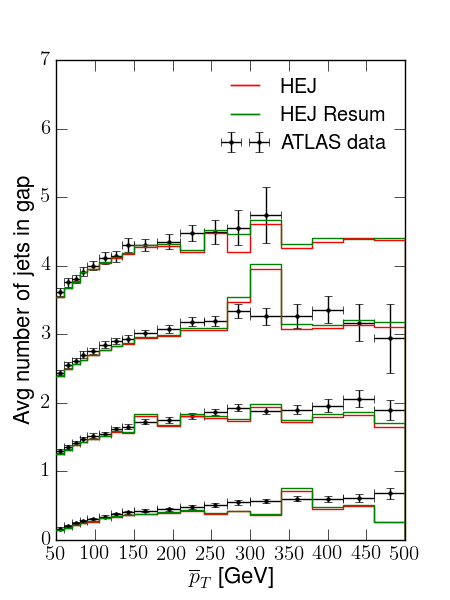
\includegraphics[scale=0.6]{Images/Veto_Plots/pf6_uno_qqx.png}}
\caption{Figure 6 of \cite{Aad2011} redone with corrections included. The red lines are the results from running the full HEJ program, the green if one only considers the resummed parts of the program and black points are the data. From the top-left: no corrections, unordered corrections, sub-leading partonic processes corrections, both corrections. In the last figure, we see how these corrections mean that there is now barely any distinction between `resummed' and `full' HEJ and that the agreement has improved to slightly higher values of $\bar{p}_T$.}
\label{fig:veto}
\end{figure}

\begin{figure}[t]
\centering
\subfloat[No NLL corrections.]{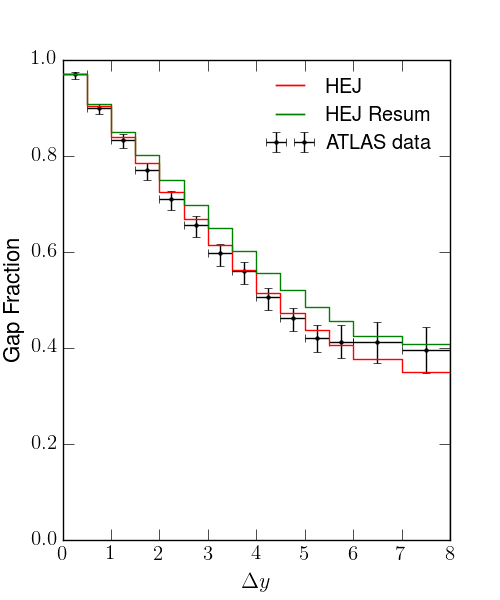
\includegraphics[scale=0.5]{Images/Veto_Plots/pf3a_bare.png}}
\subfloat[Unordered corrections.]{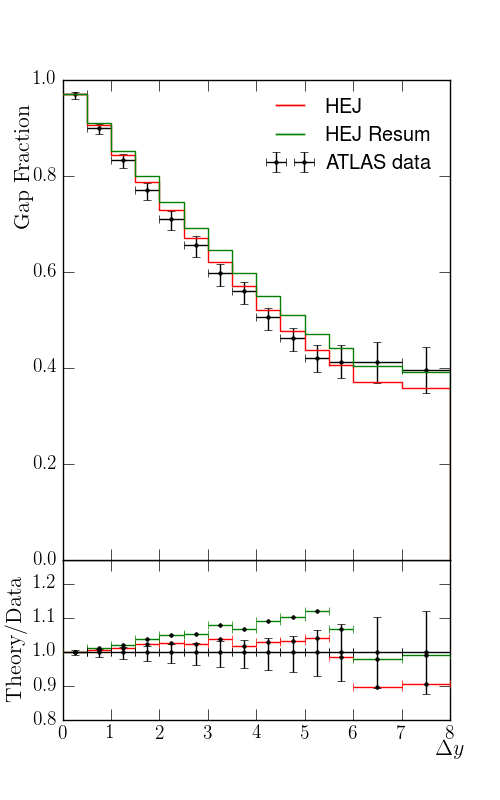
\includegraphics[scale=0.5]{Images/Veto_Plots/pf3a_uno.png}} \\
\subfloat[Sub-leading partonic processes corrections.]{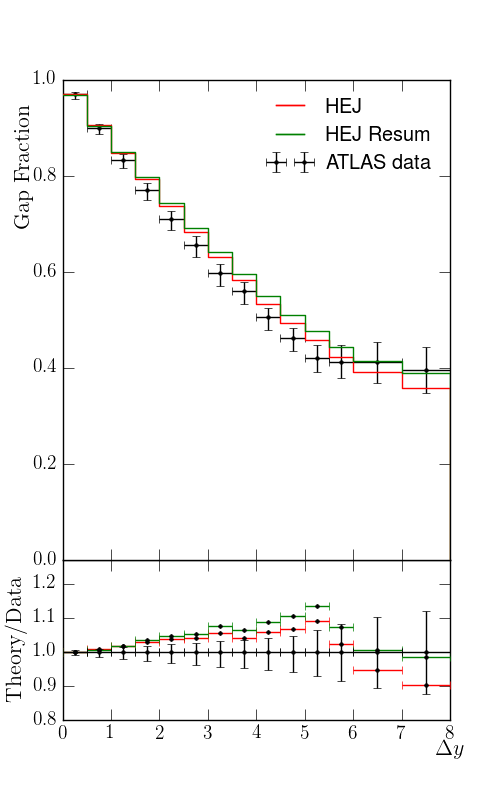
\includegraphics[scale=0.5]{Images/Veto_Plots/pf3a_qqx.png}}
\subfloat[Both corrections.]{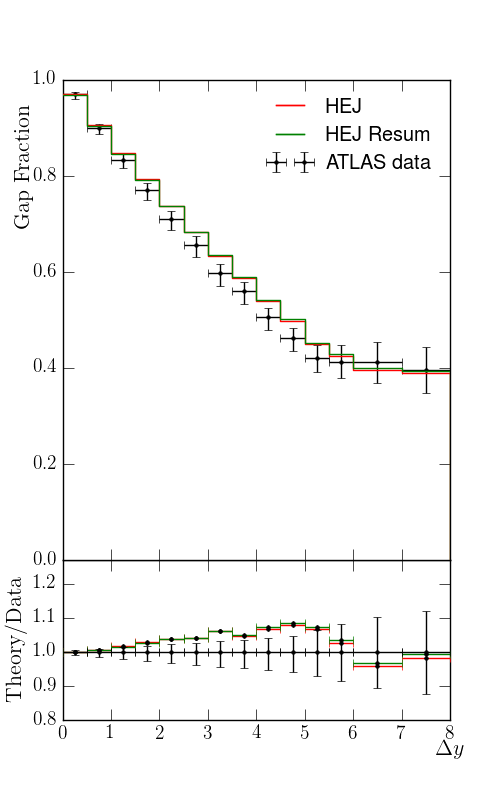
\includegraphics[scale=0.5]{Images/Veto_Plots/pf3a_uno_qqx.png}}
\caption{Figure 3a of \cite{Aad2014} redone with corrections included. The red lines are the results from running the full HEJ program, the green if one only considers the resummed parts of the program and black points are the data. Further discussion in the text.}
\label{fig:newveto3a}
\end{figure}

%Finally, we revisit a four-jet ATLAS analysis \cite{Aad2015}. This analysis is somewhat special in HEJ in that it includes matching for up to five jets in the final state (our usual approach is only up to four). To compile the fixed-order matrix elements for the five-jet matching takes on the order of days and so is not practical to do generally. However, since this analysis specifically looks at four-jet inclusive events, it was felt necessary to have the matching to this level. In figure \ref{fig:4jet}, we redo figure 4 of \cite{Aad2015}, which is a measurement of the inclusive cross section binned in leading jet $p_T$. As mentioned before, $p_T$ is generally an observable that can be tricky to match correctly with the limit we consider, but we see here that if we make an inclusive measurement, we can describe the data remarkably well. Once more, the addition of the new processes makes this measurement even better. 

%\todo{Make last figure prettier - longer, less wide, better labelling}

%\begin{figure}[t]
%\centering
%\subfloat[No NLL corrections.]{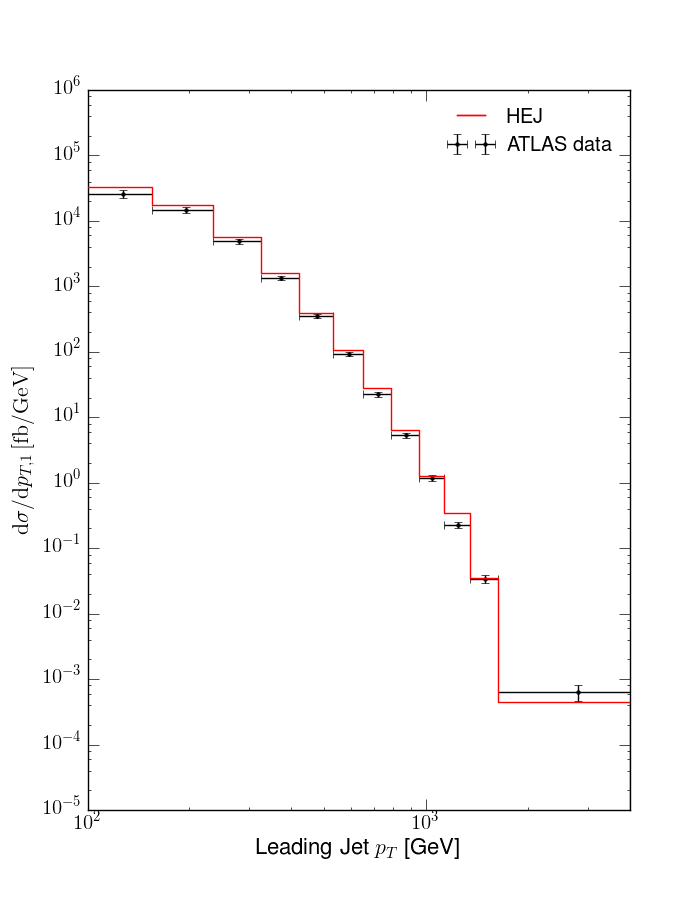
\includegraphics[scale=0.4]{Images/4j_plots/pf4_bare.png}}
%\subfloat[Unordered corrections.]{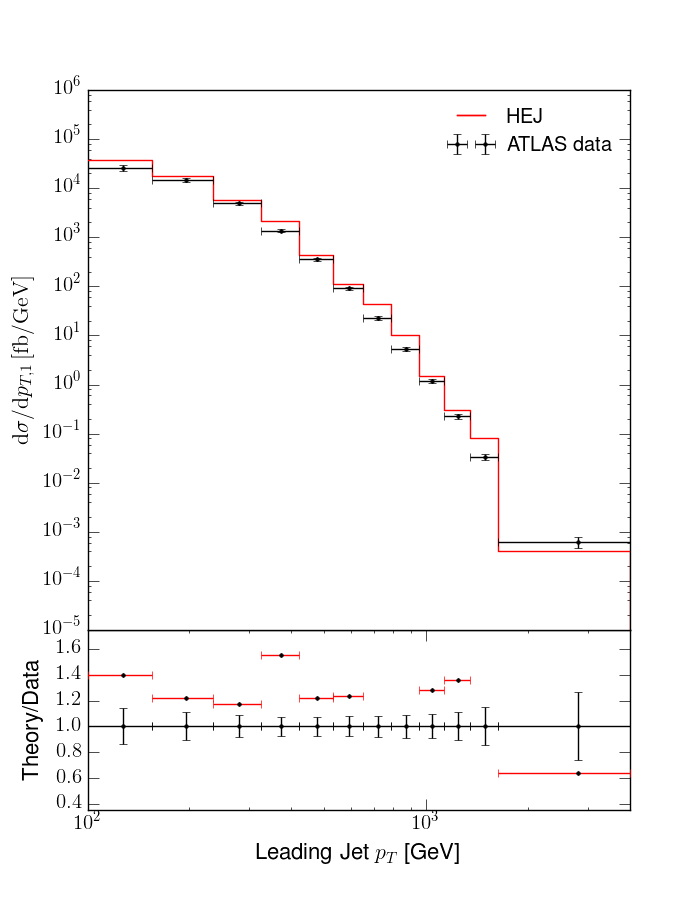
\includegraphics[scale=0.4]{Images/4j_plots/pf4_uno.png}} \\
%\subfloat[Sub-leading partonic processes corrections.]{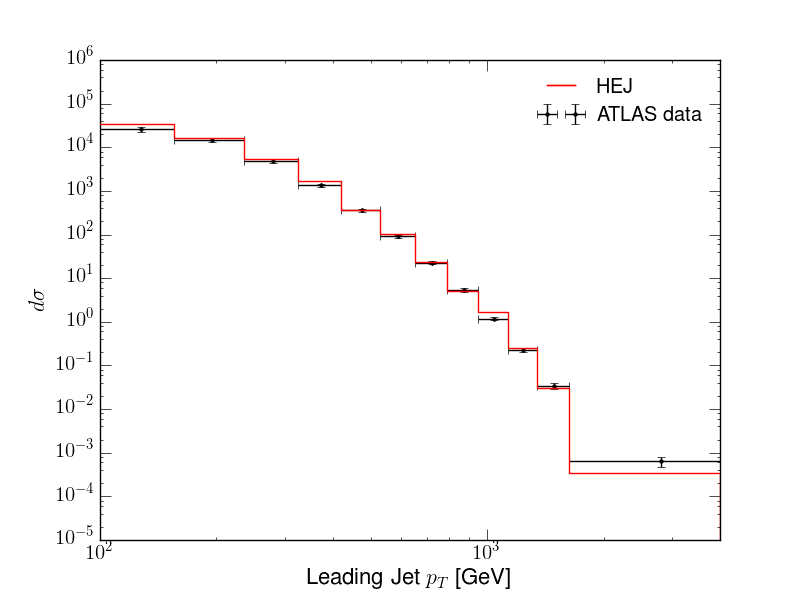
\includegraphics[scale=0.4]{Images/4j_plots/pf4_qqx.png}}
%\subfloat[Both corrections.]{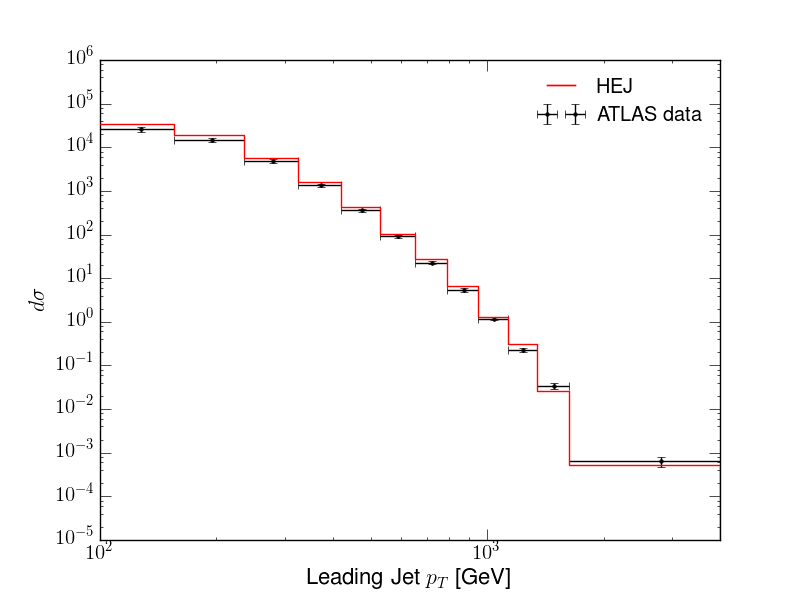
\includegraphics[scale=0.4]{Images/4j_plots/pf4_qqx_uno.png}}
%\caption{Figure 4 of \cite{Aad2015} redone with corrections included and compared. These 4-jet events are binned in the leading jet's $p_T$, which extends out to high values ($\approx 3$TeV). Despite this, HEJ tracks the data very well, especially once both the $NLL$ corrections are included.}
%\label{fig:4jet}
%\end{figure}

%\clearpage

\section{Summary}
In this chapter we have presented the beginnings of the work needed to extend HEJ to NLL accuracy. Specifically, we provided details of the calculation of so-called unordered amplitudes, where an FKL amplitude is modified such that an emitted gluon is taken outside of the previously extremal partons. Following on from that, we discussed how some inherently non-FKL amplitudes could also be included in our resummation procedure by virtue of the fact that the Lipatov ansatz holds at the next-to-leading level.

The derivation of these new amplitudes dominated the subject matter of the chapter and correctness checks such as gauge invariance and limit checks were presented as we went along. Once we were happy that the amplitudes were behaving in the way we expected, they were carefully and correctly incorporated into the HEJ program. Section 3.5 provided details of how this inclusion affected various distributions when integrating over phase space. 

The chapter concluded with comparison to real data. In all cases, it was seen that the addition of the corrections pushed our predictions closer towards the recorded data. We are now in a position to include these NLL processes as part of the standard HEJ package, forming part of the standard prediction for any future analyses. 
